% ===== INICIO DEL PREÁMBULO =====

\documentclass[msc,oneside,a4paper]{udelar} % Poner msc para Maestría, dsc para Doctorado.

\usepackage[
acronyms, 											 %utiliza el glosario de acronimos.
nohypertypes={acronym,notacion,simbolos,glosario},   %quita los links en el texto al glosario.
%nonumberlist,                                       %quita los links en los glosarios al texto.
nogroupskip,                                         %quita los espacios entre diferentes grupos dentro de un glosario.
nopostdot, 											 %quita el punto final en los acrónimos         .                           
]{glossaries}

\tolerance=1
\emergencystretch=\maxdimen
\hyphenpenalty=5
\hbadness=1


%\usepackage[titles]{tocloft}
%\setlength\cftbeforechapskip{100pt}
%\renewcommand\cftfigafterpnum{\vskip5pt\par}
%\renewcommand\cfttabafterpnum{\vskip5pt\par}
%\renewcommand\cfttabafterpnum{\hskip1pt\par}

\makeatletter
     \renewcommand*\l@figure{\@dottedtocline{1}{1em}{3.2em}}
\makeatother

%Begin FR
\newcommand{\norm}[1]{\left\Vert#1\right\Vert}
\newcommand{\abs}[1]{\left\vert#1\right\vert}
\newcommand{\set}[1]{\left\{#1\right\}}
\newcommand{\Real}{\mathbb R}
\newcommand{\eps}{\varepsilon}
\newcommand{\To}{\longrightarrow}
\newcommand{\BX}{\mathbf{B}(X)}
\newcommand{\A}{\mathcal{A}}
\newcommand{\tts}{\ensuremath(t_{1}t_{2})}
\newcommand{\esp}{\mbox{\\}}
\newcommand{\bc}{\begin{center}}
\newcommand{\ec}{\end{center}}
\newcommand{\TABH}[1]{{\mbox~}\hspace{#1mm}}
%\newcommand{\bproof}{\textbf{Proof.}~}
%\newcommand{\eproof}{\begin{flushright}\textbf{QED}\end{flushright}}
%\newcommand{\nada}[1]{}
%\newcommand{\figref}[1]{Fig-\ref{#1}}
%End FR

\usepackage{amsmath,amsfonts,amssymb,amsthm}
\newtheorem{definition}{Definition}
\newtheorem{question}{Question}
\newtheorem{theorem}{Theorem}
\newtheorem{proposition}{Proposition}
\newtheorem{property}{Property}
\newtheorem{lemma}{Lemma}
\usepackage{algorithmic}
\usepackage{algorithm}
\usepackage{tikz}
\usetikzlibrary{matrix,positioning,arrows,decorations.pathmorphing,shapes}
\usepackage{bbm}

\usepackage[T1]{fontenc}% TESTING
\usepackage{float}

%\tolerance=1
%\emergencystretch=\maxdimen
%\hyphenpenalty=10000
%\hbadness=10000

\hypersetup{ colorlinks = true } % false para imprimir, true para ver.

% Ver los documentos de estilos bibliográficos para editar estas siguientes 2 líneas.
%\usepackage{natbib} % Para algunos estilos bibliográficos
%bibliographystyle{estilos_bibliograficos/natbib/numbers/natbib_these}
\bibliographystyle{estilos_bibliograficos/natbib/numbers/acm}
\usepackage{longtable}



\loadglossary

% A su vez, la clase udelar.cls ya tiene los siguientes paquetes cargados automáticamente, que podrían ser de interés saber para el usuario:
% 
% {color},{hyphenat},{appendix},{lastpage},{babel},{inputenc},{amsmath,amssymb},{ifthen},{graphicx},{caption}
% {setspace},{tabularx},{eqparbox},{ltxcmds},{titletoc},{xcolor},{lineno},{xwatermark}

% Si se quieren agregar más paquetes, se recomienda colocarlos a partir de esta linea y antes de \begin{document}.



% ===== FIN DEL PREÁMBULO =====

% ===== INICIO DEL DOCUMENTO =====

\begin{document}



  %\title{Survivable Network Design with Reliability Constraints}
  \title{Topological Optimization of Fault-Tolerant Networks meeting Reliability Constraints}
%  \subtitle{TO BE DEFENDED}
  \institutelogo{3} % Carga cantidad de logos seleccionados, con máximo de 3 logos.
  \author{Nelson Sebasti\'an}{Laborde Castillo}
  
  \director{Ing.}{Franco}{Robledo}{Dr.}
%  \codirector{Dr.}{Franco}{Robledo}{Director de Tesis}  % Comentar estas líneas si no son necesarias.
%  \codirector{Prof.}{Nombre del 2do Codirector}{Apellido}{D.Sc.}
%  \codirector{Prof.}{Nombre del 3er Codirector}{Apellido}{D.Sc.}
  \directoracademico{Ing.}{Omar}{Viera}{Prof.}
%  \codirector {Ing.}{Pablo}{Romero}{Dr.}
  
  \examiner{Dr.}{Sebasti\'an}{Basterrech (Professor VSB-Tech. University Ostrava CZ Rep. - Revisor)}{}
  \examiner{Ing.}{Gerardo}{Rubino (Directeur de Recherche, INRIA/Rennes, Francia)}{Dr.}
  \examiner{Ing.}{Ra\'ul}{Ruggia (PEDECIBA Inform\'atica - Presidente de Mesa)}{Dr.}
%  \examiner{Prof.}{Nombre del 4to Examinador}{Apellido}{Ph.D.}
%  \examiner{Prof.}{Nombre del 5to Examinador}{Apellido}{Ph.D.}
  
  \graduatename{Inform\'atica}
  \institute{Facultad de Ingeniería}{Fing}  % La primer institución es la principal.
  \institute{PEDECIBA - Inform\'atica}{PEDECIBA}  % Agregar copias de esta línea para agregar instituciones.
  \graduatelocation{Montevideo}{Uruguay}
  
  
  \date{20}{12}{2020} % Fecha del documento.
  \foreignkeyword{Dise\~no Topol\'ogico de Redes}
  \foreignkeyword{Confiabilidad de Redes}
  \foreignkeyword{Simulaci\'on}
  \foreignkeyword{Optimizaci\'on de Redes}
  \foreignkeyword{Red Dorsal}
  \foreignkeyword{RVR}
  \foreignkeyword{Metaheur\'isticas}
  \foreignkeyword{VNS}
    
  \keyword{Topological Network Design}
  \keyword{Network Reliability}
  \keyword{Simulation}
  \keyword{Network Optimization}
  \keyword{Backbone}
  \keyword{RVR}
  \keyword{Metaheuristics}
  \keyword{VNS}

        
  \maketitle  % Comando que genera el título de la tesis.
  
  \frontmatter  % Comando que genera la portadilla, el catalogo y el tribunal de evaluación. NO COMENTAR
  
  \dedication{(Dedicatoria) A mis Padres Ricardo y Rosario, a mi Hermano Santiago y a mi Familia.}


  \chapter*{Agradecimentos}

Quisiera agradecer a mis tutores, Dr. Ing. Franco Robledo y Prof. Ing. Omar Viera, por el apoyo, gu\'ia y gran paciencia durante todo el proceso de desarrollo de esta Tesis.\\ \\

Agradezco la participación del Dr. Ing. Pablo Romero en el intercambio de ideas y su colaboraci\'on en la revisi\'on y mejora de este trabajo.\\ \\

Agradezco a Ing. Sebasti\'an Ressi e Ing. Alvaro Rivoir por su colaboraci\'on con ideas y sugerencias, basadas en su experiencia con trabajos previos, en la misma tem\'atica que el presente trabajo.\\ \\

Agradezco profundamente el honor de tener al Dr. Sebasti\'an Basterrech como revisor de este trabajo.
\\ \\

A mi amigo y colega Ing. Julio Cesano por alentarme a inscribirme junto a \'el, en el programa de Maestr\'ia PEDECIBA.
\\ \\

Un agradecimiento muy especial a mi familia, a mi esposa Mara y a mis hijos Maite y Guillermo, por todo el apoyo, comprensi\'on y motivaci\'on que me dieron durante el desarrollo de este trabajo, el cu\'al est\'a enteramente dedicado a ellos.

%  \include{ded_agr_epi/epigrafe}
  \begin{foreignabstract}
En una red las entidades relevantes son nodos y conexiones entre nodos, y en general el principal objetivo buscado es lograr una comunicaci\'on segura entre nodos de esta red, ya sea para redes telef\'onicas y de comunicaci\'on de datos, de transporte, arquitectura de computadores, redes de energ\'ia el\'ectrica o sistemas de comando y control. 
La optimizaci\'on relativa al costo de una red y la confiabilidad de la misma, relacionada con la supervivencia de esta, son los criterios predominantes en la selecci\'on de una soluci\'on para la mayor parte de los contextos. Un tema interesante que ha atra\'ido un gran esfuerzo es c\'omo dise\~nar topolog\'ias de red, con un uso m\'inimo de recursos de red en t\'erminos de costo que brinde una garant\'ia de confiabilidad. A pesar que por a\~nos el costo ha sido el factor primario, la confiabilidad ha ganado r\'apidamente en relevancia. Con sistemas de transmisi\'on de fibra \'optica de alta capacidad formando la columna vertebral de la mayor\'ia de las redes actuales y junto con el r\'apido desarrollo de la tecnolog\'ia de comunicaci\'on de redes y el crecimiento explosivo de las aplicaciones de Internet, la confiabilidad de la red parece cada vez m\'as importante, tanto para \'areas tradicionales como la industria de defensa, finanzas y energ\'ia, y \'areas emergentes como la computaci\'on confiable, la computaci\'on en la nube, internet de las cosas (IoT) y la pr\'oxima generaci\'on de Internet, la supervivencia del tr\'afico por sobre los fallos de red se ha convertido a\'un en m\'as cr\'itica.
En ese sentido podemos diferenciar, a grandes rasgos, dos de los principales problemas a resolver en el an\'alisis y dise\~no de topolog\'ias de red. Primeramente la obtenci\'on de una red \'optima en alg\'un sentido, siendo este definido por ejemplo mediante la obtenci\'on de la m\'axima cantidad posible de caminos disjuntos entre pares de nodos, esto sujeto a determinadas restricciones definidas seg\'un el contexto. El segundo problema es la evaluaci\'on de la confiabilidad de la red en funci\'on de las confiabilidades elementales de los nodos y conexiones entre nodos que componen la red. Estas confiabilidades elementales son probabilidades de operaci\'on asociadas a los nodos y conexiones entre nodos. Ambos problemas est\'an fuertemente relacionados, pudiendo tener que comparar en el proceso de b\'usqueda de redes \'optimas la confiabilidad entre soluciones candidatas, o luego de obtener una soluci\'on candidata tener que evaluar la confiabilidad de la misma y de esta forma descartarla o no.
El presente trabajo se centra en la resoluci\'on del problema enfocado en ambos puntos planteados. Para ello modelamos el problema de dise\~no de la topolog\'ia de red sobre la base de un modelo definido como Generalized Steiner Problem with Node-Connectivity Constraints and Hostile Reliability (GSP-NCHR) extensi\'on del m\'as conocido Generalized Steiner Problem (GSP).
El presente problema es $\mathcal{NP}$-duro, dedicamos un cap\'itulo para presentar resultados te\'oricos que lo demuestran. Nuestro objetivo es atacar de forma aproximada el modelo GSP-NCHR de tal modo de poder resolver la optimizaci\'on de la red y luego medir la confiabilidad de la soluci\'on obtenida. Para ello optamos por desarrollar la metaheur\'istica Variable Neighborhood Search (VNS). VNS es un m\'etodo potente que combina el uso de b\'usquedas locales basadas en distintas definiciones de vecindad, el cual ha sido utilizado para obtener soluciones de buena calidad en distintos problemas de optimizaci\'on combinatoria. 
En lo referente al c\'alculo de confiabilidad de la red, nuestro modelo GSP-NCHR pertenece a la clase $\mathcal{NP}$-duro, por eso desarrollamos Recursive Variance Reduction (RVR) como m\'etodo de simulaci\'on, ya que la evaluaci\'on exacta de esta medida para redes de tama\~no considerable es impracticable. 
Las pruebas experimentales fueron realizadas utilizando un conjunto amplio de casos de prueba adaptados de la librer\'ia travel salesman problem (TSPLIB), de heterog\'eneas topolog\'ias con diferentes caracter\'isticas, incluyendo instancias de hasta 400 nodos. Los resultados obtenidos indican tiempos de 
c\'omputo altamente aceptables acompa\~nados de \'optimos locales de buena calidad.

\end{foreignabstract}

Como resultado de esta tesis, se ha logrado la siguiente publicaci\'on: "A GRASP/VND Heuristic for the Generalized Steiner Problem with Node-Connectivity Constraints and Hostile Reliability" que ser\'a publicada en \textit{"Proceedings of the 8th International Conference on Variable Neighborhood Search (ICVNS Marzo 2021). Khalifa University, Abu Dhabi, U.A.E." Este art\'iculo ser\'a publicado por Springer en "Lecture Notes in Computer Science (LNCS) series."}


  \begin{abstract}
The relevant entities in a network are its nodes, and the links between them. In general, the goal is to 
achieve a reliable communication between different pairs of nodes. Examples of applications are telephonic services, data communication, transportation systems, computer systems, electric networks and control systems. 

The predominant criterion for the design of a reliable and survivable system is the minimum-cost in most contexts. 
An attractive topic for research is to consider a minimum-cost topological optimization design meeting a  reliability threshold. Even though the cost has been the primary factor in the network design, recently, the network reliability has grown in relevance. With the progress of Fiber-To-the-Home (FTTH) 
services for the backbone design in most current networks, combined with the rapid development of network 
communication technologies, and the explosive increase of applications over the Internet infrastructure, the network reliability has supreme importance, for traditional communication systems but for the defense, business and energy, and emergent fields such as trusted computing, cloud computing, Internet of Things (IoT) and Next Generation Networks (NGN), the fault tolerance is critical.  

We can distinguish two main problems to address in the analysis and design of network topologies. First, the robustness is usually met under multi-path generation. Therefore, we require certain number of node-disjoint paths between distinguished nodes, called terminals. The second problem is to meet a minimum-reliability requirement in a hostile environment, using the fact that both nodes and links may fail. Both problems are strongly related, 
where sometimes the minimum-cost topology already meets the reliability threshold, or it should be discarded, and 
the design is challenging. 
 
This thesis deals with a topological optimization problem meeting reliability constraints. The 
Generalized Steiner Problem with Node-Connectivity Constraints and Hostile Reliability (GSP-NCHR) 
is introduced, and it is an extension of the well-known Generalized Steiner Problem (GSP). Since GSP-NCHR  
subsumes the GSP, it belongs to the class of $\mathcal{NP}$-Hard problems. A full chapter is dedicated to the hardness of the GSP-NCHR, and an analysis of particular sub-problems. Here, the GSP-NCHR is addressed approximately. Our goal is to meet the topological requirements intrinsically considered in the GSP-NCHR, and then test if the resulting topology meets a minimum reliability constraint. 

As a consequence a hybrid heuristic is proposed, that considers a Greedy Randomized construction phase followed by a Variable Neighborhood Search (VNS) in a second phase. VNS is a powerful method that combines local searches 
that consider different neighborhood structures, and it was used to provide good solutions in several hard combinatorial optimization problems. Since the reliability evaluation in the hostile model belongs to 
the class of $\mathcal{NP}$-Hard problems, a pointwise reliability estimation was adopted. Here we considered 
Recursive Variance Reduction method (RVR), since an exact reliability evaluation is prohibitive for large-sized networks. 

The experimental analysis was carried out on a wide family of instances adapted from travel salesman problem library (TSPLIB), for heterogeneous networks with different characteristics and topologies, including up to 400 nodes. The numerical results show acceptable CPU-times and locally-optimum solutions with good quality, meeting network reliability constraints as well.\\\\

\textbf{Keywords}:
\end{abstract}
\\
\\
\\
\begin{normalsize}
As product of this thesis, the following publication has been achieved: "A GRASP/VND Heuristic for the Generalized Steiner Problem with Node-Connectivity Constraints and Hostile Reliability" to be published in the     \textit{"Proceedings of the 8th International Conference on Variable Neighborhood Search (ICVNS March 2021). Khalifa University, Abu Dhabi, U.A.E. The article will be published by Springer in the Lecture Notes in Computer Science (LNCS) series."}
\end{normalsize}
  
%  \listoffigures	         % Lista de figuras
%  \listoftables	         % Lista de tablas
  
%  \listadesimbolos 		     % Lista de símbolos
  %\listadenotaciones 	     % Lista de notaciones
  \listadesiglas 		     % Lista de siglas

  \tableofcontents           % Tabla de contenidos

  \mainmatter % Comando que genera las listas y capítulos. NO COMENTAR
  
  \chapter*{Glossary}
\begin{itemize}
\item \textbf{GSP}: Generalized Steiner Problem.
\item \textbf{GSP-NC}: GSP with Node-Connectivity Constraints.
\item \textbf{GSP-EC}: GSP with Edge-Connectivity Constraints.
\item \textbf{GSP-NCHR}: GSP with Node-Connectivity Constraints and Hostile Reliability.
\item \textbf{GSP-ECHR}: GSP with Edge-Connectivity Constraints and Hostile Reliability.
\item \textbf{SNDP}: Survivable Network Design Problem.
\item \textbf{GSNDP}: Generalized Survivable Network Design Problem.
\item \textbf{GNDP}: Generalized Network Design Problem.
\item \textbf{VCSNDP}: Vertex Connectivity Survivable Network Design Problem.
\item \textbf{SN-MSP}: Survivable Network with Minimal Steiner nodes Problem.
\item \textbf{SMT}: Steiner Minimal Tree.
\item \textbf{MCSP}: Minimal Connected Sub Graph Problem.
\item \textbf{MST}: Minimum Spanning Tree.
\item \textbf{TSP}: Travel Salesman Problem.
\item \textbf{BNDP}: Backbone Network Design Problem.
\item \textbf{KSP}: K Shortest Paths.
\item \textbf{WAN}: Wide Area Network.
\item \textbf{IP}: Internet Protocol.
\item \textbf{MPLS}: Multiprotocol Label Switching.
\item \textbf{ZDD}: Zero Decision Diagram.
\item \textbf{CMC}: Crude Monte Carlo.
\item \textbf{RVR}: Recursive Variance Reduction.
\item \textbf{RNN}: Random Neural Network.
\item \textbf{SMBS}: Stochastic Monotone Binary System.
\item \textbf{GRASP}: Greedy Randomized Adaptive Search Procedure.
\item \textbf{IoT}: Internet of Things.
\item \textbf{GA}: Genetic Algorithm.
\item \textbf{RL}: Relocation Heuristics.
\item \textbf{VNS}: Variable Neighborhood Search.
\item \textbf{ILS}: Iterated Local Search.
\item \textbf{TS}: Tabu Search.
\item \textbf{VND}: Variable Neighborhood Descent.
\item \textbf{VNDS}: Variable Neighborhood Decomposition Search.
\item \textbf{BVNS}: Biased Variable Neighborhood Search.
\item \textbf{PVNS}: Parallel Variable Neighborhood Search.
\end{itemize}  % Se carga el glosario
  \chapter{Introduction}\label{intro}
\section{Context}
This thesis is developed for the Master in Informatics, under the Program for the Development of Basic Sciences (PEDECIBA), and Universidad de la Rep\'ublica (UdelaR). This work is developed under the framework of a more general network planning project for modern communication networks. This is generally a complex and demanding task, which is accomplished by optimization as a main tool, and combines a quantitative analysis and evaluation as a primary element in the cycle of optimization. In this thesis, we wish to develop a research activity that includes the design of highly-reliable massive telecommunication networks. Given the previous experience in this field, it is essential to assist on decision-making, which is extremely useful for the design of fiber-optics communications. 

The information revolution shocked the world during the XX and XXI centuries, and it represents one of the most relevant revolutions in history. The impact was even greater when sharing digital information, allowing  cooperation and convergence between both technologies and people. At the beginning, telephonic 
networks\footnote{Network: it can be considered as a set of nodes and a set of links between them.} were 
considered to satisfy the data communication needs. Currently, the situation is much different, and data networks were adapted to pursue different goals, normally by means of service integration and traffic needs. 
The data networks allow the multiple convergence of different communication technologies permanently, even when the original deployment has more than a century. The interconnection allows hub, storage and centrality of information that is sparse among distinct continents. As a result, jobs, e-commerce, business and other routine activities are speed-up, and a great variety of on-line services are available anytime and anywhere, with anything at hand (i.e., a cell-phone). The network design task, combining different traffic and services, among many other factors, is not easy at all, but the contrary. This task is complex, and the design, network dimensioning and optimization\footnote{Optimization: a field of mathematics that assists on decision making, by means of a minimization/maximization of a quantity, using a specific criterion.} represents hard decisions to make. 
This complex task must be simultaneously accomplished with the development of a network topology\footnote{Network Topology: physical configuration in which nodes are interconnected in a network.} that meets a specific reliability threshold\footnote{Reliability: the probability of correct operation of a system on given conditions during a specific period of time.} suitable for the context. A large number of sites with different characteristics are interconnected during the network design, in order to meet a pre-established reliability bound at the minimum cost. 

The goal in every topological design\footnote{Topological design: stage of the network planning process  which consists in the physical location of the network components and their interconnections.} is to adapt the technological requirements from the context as much as possible, meeting the budget constraints 
imposed by the project (which implies the cost of infrastructure but also factors related with an expected quality of service). In this work we address a topological design of highly-reliable networks\footnote{Structural Reliability: probability of correct operation of a system, given the occurrence of failures on the network components.}, adding different optimization phases by means of quantitative evaluations in order to determine if the desired reliability parameter is achieved.

\section{Problem}
During the first phase of this thesis, a literature review was performed. As a result, we defined the problem under study with the following two items:
\begin{itemize}
    \item Given a network where the potential link-costs are known, design a minimum-cost network meeting predetermined connectivity and reliability constraints (inputs of the problem).
    \item Perform a quantitative analysis of the results, in terms of cost.
\end{itemize}
In this context, it is relevant to dispose of methods for the topological network design meeting certain 
connectivity requirements (i.e., two node-disjoint paths between nodes) and simultaneously, some 
network reliability requirement (measured in probabilistic terms) exceeding a predefined threshold (problem data). The problem involves a mixture of structural reliability and topological survivability\footnote{Topological survivability: is to accomplish certain network connectivity levels.} of a network. 
In a first phase, a literature review is performed and, in a second phase, different solutions to the problem are proposed. The third phase is the implementation of the selected methodology. Finally, in the fourth phase, 
an experimental analysis is carried out to measure quantitatively the quality of the solution obtained following the designed methodology, and to determine, if possible, \emph{how good} are the returned solutions.  

\section{Goals}
\subsection{General Goal}
Develop a heuristic\footnote{Heuristic: method and exploratory algorithms for the resolution of problems, where the solutions are discovered as a result of the progress achieved during a  search.} whose result is the design of a network topology (i.e., associated graph) meeting 
connectivity requirements between pairs of nodes (problem data) and a minimum reliability threshold 
(problem data). Answer key-questions, in order to understand the interplay 
between topological survivability and structural network reliability.

\subsection{Specific Goals}
The author of this thesis is proposed to perform an in-depth study of the concepts of 
\emph{Structural Reliability} and \emph{Topological Survivability}. 
A specific goal is to get skills in network reliability and planning, particularly on the topological design 
of strategic complex networks with critical/relevant applications~\cite{31}. Learn network planning tools and how to 
implement efficient algorithms to tackle $\mathcal{NP}$-Hard problems\footnote{$\mathcal{NP}$-Hard: so far, these problems cannot be solved efficiently (in polynomial-time with respect to the size of the input).}, such as the problem addressed in this thesis.

\section{Expected Results}
Macroscopically, it is expected to offer a methodology that serves as a base-step for decision-making 
in the development of fault-tolerant telecommunication networks. This is typically the case of a backbone network 
design\footnote{Backbone: is the skeleton or main core of a network.} of a Wide Area Network (WAN),  
    (i.e., Internet). In order to meet these objectives, the following tasks should be performed:
\begin{itemize}
    \item Understand the mathematical model associated to the problem to solve.
    \item Perform a literature review.
    \item Get a better insight of the following concepts:
           \begin{itemize}
               \item Topological network survivability.
               \item Structural network reliability.
           \end{itemize}
    \item Explore different approaches to propose an approximate solution.
    \item Select and implement a solution.
    \item Measure the quality of the results obtained.
\end{itemize}

\section{Methodology}
In a previous stage to the development of a solution for the problem, the author performed a literature review, understanding the main concepts and related fields of knowledge. 
As far as I know, the object under study in this thesis is novel. I can find a scarce number of close  problems from the scientific literature. In fact, the closest works from the literature either deal with 
network reliability, or network optimization independently, but not both. The first stage of this project is focused on understanding the problem and propose a formal (mathematical programming) definition. Given that, the problem under study belongs to the $\mathcal{NP}$-Hard class, an exact evaluation algorithm is prohibitive for large networks. As a consequence, a metaheuristic is adopted. In terms of the optimization problem, several metaheuristics were studied to potentially address the problem\footnote{Metaheuristic: particular heuristics that serve as a template to solve a very large class of computational problems.}. Among those metaheuristics we can find GRASP~\cite{5,6,51} and its particular version for 
GSPNC~\cite{2,11}, Genetic Algorithms~\cite{1,5},  Tabu Search~\cite{5,15}, Variable Neighborhood Search or VNS~\cite{16,17,18} and Iterated Local Search, or ILS~\cite{5,19,60}. The selection of a metaheuristic provides opportunities to use a powerful and flexible tool, that can be easily combined with 
hybrid method or specific heuristics suitable for the problem. Once analyzed and understood a variety of potential metaheuristics for our network optimization problem (the construction phase of our topological network design), 
the decision was to adopt VNS. This metaheuristic is 
based on a simple principle: a systematic variation of neighborhood structures during the search. 
The accuracy to switch neighborhood structures is essential. VNS has shown its effectiveness by means of several experiments showing equal or better results than most metaheuristics for a great variety of combinatorial optimization problems, which makes this selection attractive.

Analogously, for the stage of network reliability analysis, different evaluation techniques were studied. 
An exact network reliability evaluation belongs to the 
class of $\mathcal{NP}$-Hard problems, for our hostile model of simultaneous links and node-failures. 
Therefore, simulation methods were considered\footnote{Simulation: is to perform repetitions of a model under a fixed assumption.}, such as Crude Monte Carlo, or CMC~\cite{4} and 
Recursive Variance Reduction or RVR~\cite{85,2,78}. Even though Crude Monte Carlo proposed an unbiased reliability estimation, this technique is not suitable for highly reliable scenarios, since it does not satisfy the property of bounded relative error. An outstanding method for variance reduction is RVR, which was selected in this thesis. 
The implementation is not trivial, but there is both, practical and theoretical evidence that RVR presents much reduced variance than CMC~\cite{80}. In practice, RVR is suitable for the reliability estimation on large networks,  
even under highly reliable scenarios~\cite{79}.

\section{Conclusions}
In this thesis we study the topological design of highly-reliable networks, tackling two sub-problems clearly identified: the network optimization problem and the minimum network reliability requirements. The network optimization problem is here addressed using metaheuristics, since it is an $\mathcal{NP}$-Hard problem~\cite{9,27,29}, and therefore, the application of exact methods is prohibitive in terms of computational time, even for networks with small and moderate size. For that reason, we decided to adopt Variable Neighborhood Search, 
(VNS). The reasons to support this decision will be exposed in Chapter~\ref{prob-def}. In terms of the 
network reliability evaluation method, simulation methods are used, since exact reliability evaluation methods are also prohibitive. The Recursive Variance Reduction (RVR) method was selected for the pointwise reliability estimation in our hostile environment of simultaneous link/node failures. The reasons to select RVR are also discussed in Chapter~\ref{prob-def}. We do not have access to public benchmark data for our network optimization problem\footnote{Benchmark: technique used to measure the performance of a system or part of it, commonly in relation with a parameter of reference.} in order to compare the quality of the results, having to simulate network test instances. Nevertheless, 
the CPU-times are acceptable, and the returned solutions are locally-optimal, with good quality in terms of costs reduction.  
It is worth to note that the related literature from the scientific community is scarce, and the problem under study is novel. 

\section{Structure of this Thesis}
This thesis is organized in the following manner. Chapter~\ref{intro} serves as an introduction, and contains the motivation of this thesis, some elements of the problem under study and comments on the selected methodology for its resolution. Chapter~\ref{background} presents the terminology that will be used throughout this thesis. A 
description of the problem and reasons to select VNS and RVR as the building-blocks of our resolution is provided in Chapter~\ref{prob-def}. Chapter~\ref{problem} formally presents the 
Generalized Steiner Problem with Node-Connectivity Constraints and Hostile Reliability (GSP-NCHR) 
with a mathematical programming formulation. Its $\mathcal{NP}$-Hardness is established, and particular cases are also discussed. The related work for the selected resolution methods is covered in Chapter~\ref{related}. 
Full details of the algorithmic resolution is presented in Chapter~\ref{algorithms}. The experimental tests  
together with a quantitative analysis of the results is included in Chapter~\ref{results}. 
Chapter~\ref{conclusions} presents Concluding remarks, and Chapter~\ref{future} points out trends for future work and possible research fields that extend or complement this thesis. An Appendix is devoted to validation tests, some special procedures involved in the algorithmic design and a visualization tool for graphs that is also a product of this thesis.
In order to experimental reproducibility the source code, data testset and other materials are available at \url{https://github.com/slaborde/NetworkDesign} % Se carga el capítulo 01
  \chapter{Background}\label{background}
This chapter includes the basic terminology from Network Optimization, Complexity and 
Graph Theory that will be used throughout this thesis. The reader is invited 
to consult the books~\cite{25,3,4,7} for additional terminology.


\section{Concepts on Network Optimization}
\begin{enumerate}
	 \item \emph{Graph}: a set of nodes and links between them. The links could be directed; in that case we have a \emph{directed graph}. 
    \item \emph{Network}: a weighted graph, where the weight is a function on the nodes and/or links that represent either costs, capacities or probabilities. 
    \item \emph{Backbone}: is the skeleton or main core of a network. A fixed network could have more than 
    one backbone (i.e., Internet). 
    \item \emph{Reliability}: is the probability of correct operation of a system.
%    \item \emph{Structural Reliability}: is the probability that the network is operational, 
%    even under network failures (i.e., connectedness). The reliability is a function of the elementary 
%    reliabilities of the network components.
%    \item \emph{Network Topology}: is a set composed by the links that connect nodes from the network. The topology is uniquely determined by the configuration of the connections between the nodes 
%    (i.e., Ring, Mesh, Star, Fully Connected, Line, Tree, Bus).
    \item \emph{Topological Design}: stage of the network planning process, which consists of 
    the location of the network components and their interconnections.
    \item \emph{Survivability}: is the ability of a system, sub-system, equipment, process or procedure of 
    its correct functioning during and after an alteration.
    \item \emph{Topological Survivability}: is to meet certain network connectivity levels of the network. 
It is precisely the existence of a pre-established number of node-disjoint (or link-disjoint) 
paths between every pair of terminal nodes.
    \item \emph{Heuristic}: exploration methods or algorithms to solve problems, where the solutions are 
    discovered by the evaluation of the progress achieved during the search of a final result. Even though the 
    exploration is algorithmic, an evaluation is empirical. They are normally employed to address hard combinatorial optimization problems, and trade optimality for computational feasibility. 
    \item \emph{Metaheuristic}: particular heuristics that serve as a template to solve a very large class of computational problems. %Metaheuristics are generally applied to problems where there are no specific exact algorithms to solve it.
    \item \emph{Optimization}: maximization of an objective function (e.g., gains, velocity, efficiency, others),  or minimization (e.g., cost, time, risk, error, others) subject to a feasible set of one or multiple constraints. 
The constraints mean that not every decision (solution) is feasible. In systems engineering, an optimization process implies the enhancement of a system, with the available resources (bandwidth, CPU, memory, etc.). 
    \item \emph{Combinatorial Optimization}: an optimization problem where the feasible set is finite. 
%    This is a field of optimization in applied mathematics and computer science, related with operations research, algorithmic theory and complexity theory, that is supported by the intersection of several fields of knowledge such us artificial intelligence, mathematics and software engineering. The algorithms efficiently explore the finite space of feasible solutions with large cardinality. 
    \item Locally-optimum solution: best solution in a set of neighbor solutions.
    \item Globally-optimum solution: best solution in the solution feasible set~\footnote{Is the set of all possible points (sets of values of the choice variables) of an optimization problem that satisfy the problem's constraints, potentially including inequalities, equalities, and integer constraints.}.
    \item $\mathcal{NP}$: is the set of decision problems that can be solved in polynomial-time by a non-deterministic Turing machine. 
    \item $\mathcal{NP}$-Hard: the set of problems $H$ such that every problem $L \in \mathcal{NP}$ can be 
    reduced to $H$ in polynomial-time. An~$\mathcal{NP}$-Hard problem is at least as hard as any problem in the 
    class $\mathcal{NP}$. In fact, if we solve a problem from the class~$\mathcal{NP}$-Hard, then we can 
    solve all the problems from the $\mathcal{NP}$ class. 
    \item $\mathcal{NP}$-Complete: the set of $\mathcal{NP}$ decision problems that belong to the 
    $\mathcal{NP}$-Hard class. 
    This class represents the hardest decision problems belonging to the $\mathcal{NP}$-class.   
    \item \emph{Simulation}: repetitive experimentation with a model with a fixed hypothesis.
   \item \emph{Greedy Algorithm}: iteratively picks the cheapest item, in order to build the best solution of a combinatorial optimization problem. In most cases, Greedy does not find the globally-optimum solution, but a good approximation.
   \item \emph{Neighborhood}: a set of solutions that include a specific member $x$. We can freely use these neighborhood, meeting the following clauses:
   \begin{itemize}
    \item $x$ belongs to all its neighborhoods. 
    \item A set that contains a neighborhood of $x$ is also a neighborhood. 
    \item The intersection of two neighborhoods of $x$ is also a neighborhood. 
    \item For every neighborhood $V$ of $x$, there exists another neighborhood $U$ of $x$ such that $V$ 
    is a neighborhood of all the points of $U$.  
   \end{itemize}
\end{enumerate}

\section{Graph-Theoretic Terminology}
In this section we present basic graph-theoretic terminology that will be used throughout this thesis~\cite{11}.

\begin{enumerate}
\item \emph{Adjacency}: two nodes $u$ and $v$ are adjacent if the link $\{u,v\}$ belongs to the graph. 
In directed graphs the order matters, and we denote $(u,v)$ to the ordered pair. 
We also say that the link $\{u,v\}$ is adjacent to both nodes $u$ and $v$.

\item \emph{Degree}: the degree $d(v)$ of a node $v$ is the number of adjacent links to $v$.
A node is isolated if it has degree 0. 

\item \emph{Induced graph}: given a graph $G=(V,E)$ and a set $U \subseteq V$, 
the induced graph $G(U)$ denotes the graph in the node-set $U$, with those links 
from $G$ whose extremes are included in $U$.

\item \emph{Path}: non-empty graph $P=(V,E)$ such that $V=\{v_1,\ldots,v_k\}$ and 
$E=\{(v_1,v_2),(v_2,v_3),\ldots,(v_{k-1},v_k)\}$. The nodes $v_1$ and $v_k$ 
are connected by $P$, and $v_1$ and $v_k$ are the extremes of $P$. The remaining nodes are internal nodes.

\item \emph{Cycle}: given a path $P=\{v_1,\ldots,v_k\}$, the graph $C$ 
obtained by the concatenation between $P$ and $\{v_k,v_1\}$ is a cycle. 

\item \emph{Node-Disjoint Path}: two paths $p$ and $q$ are node-disjoint if $p \cap q = \{v_1,v_k\}$, 
being $v_1$ and $v_k$ the extremes of both $p$ and $q$. A generalization for multiple disjoint paths is straight. 

\item \emph{Independent Paths}: two paths $p_1$ and $p_k$ are independent if $p_1 \cap p_k = \emptyset$, 
this is, $p_1$ and $p_k$ do not share nodes in common.

%\item Caminos nodo-disjuntos (con los mismos extremos): Dados dos caminos incluidos en un grafo con los mismos extremos decimos que  son nodo-disjuntos si la intersecci\'on de sus conjuntos de nodos internos es vac\'ia.

\item \emph{Subgraph}: given a graph $G=(V,E)$, $H=(V^{\prime},E^{\prime})$ is a subgraph of $G$ if $V^{\prime} \subseteq V$, $E^{\prime} \subseteq E$ and $\forall (u,v) \in E^{\prime}$, $u,v \in V^{\prime}$. 

\item \emph{Connected Graph}: a graph $G=(V,E)$ is connected if for each pair of nodes 
$u,v \in V$ there exists a path that connects $u$ and $v$ in $G$. 

\item \emph{Tree}: a graph $G=(V,E)$ is a tree if it is connected and for all the links $e\in E$, 
the graph $G^{\prime}=(V,E \setminus \{e\})$ is not connected.

\item \emph{Spanning Tree}: given a connected graph $G=(V,E)$, a subgraph $H=(V,E^{\prime})$ is a 
spanning tree if $H$ is connected and for all the links $e \in E^{\prime}$,   
$H^{\prime} = (V,E^{\prime} \setminus \{e\})$ is not connected. 

\item \emph{$k$-Node Connectivity}: a graph $G=(V,E)$ is $k$-node connected if for all $u,v \in V$, 
there exist at least $k$ node-disjoint paths in $G$ that connect them.

\item \emph{Terminal nodes}: a distinguished node-set $T$ that belongs to the backbone 
are called terminal-nodes or fixed nodes. These nodes generally correspond to access points in the local networks.

\item \emph{Matrix with the connectivity requirements}:  $R=\{r_{i,j}\}_{i,j\in T}$ 
is a matrix that stores, for every pair of terminal nodes $i,j \in T$, a non-negative integer $r_{i,j}$. 
The requirement $r_{i,j}$ means that we must construct $r_{i,j}$ node-disjoint paths 
between the terminal nodes $i$ and $j$.  

\item \emph{Backbone Network Design Problem (BNDP)}: given a network $G_B$ equipped with a terminal-set $T$, 
find the minimum-cost network $H_B \subseteq G_B$ 
that meets the connectivity requirements $R$ for the terminal-nodes $T$.

\item \emph{Key-node}: consider a feasible solution $G_{sol}$ that meets the connectivity requirements $R$. 
A key-node is a non-terminal node $v \in V$, whose degree $d(v)$ is three or greater. 

\item \emph{Key-path}: consider a feasible solution $G_{sol}$ that meets the connectivity requirements $R$.  
A  key-path is a path belonging to $G_{sol}$, such that the internal nodes are non-terminal nodes 
with degree 2, and whose extremes are either terminals or key-nodes.

\item \emph{Key-tree}: consider a feasible solution $G_{sol}$ that meets the connectivity requirements $R$, 
and $v \in G_{sol}$ a key-node. The key-tree rooted at $v$ is the tree composed by all the 
key-paths belonging to $G_{sol}$ where $v$ is one of the extremes. Topologically, this is a set of 
key-paths that share a key-node as a common extreme.
\end{enumerate} % Se carga el capítulo 02
  \chapter{Problem Definition}\label{prob-def}
\section{Motivation}
Recently, the traditional design of copper lines, the redundancy and survivability~\footnote{Survivability: is the ability of a system, sub-system, equipment, process or procedure of 
    its correct functioning during and after an alteration.} were not consider a relevant issue. This is due to the fact that multiple routes were mandatory, given the limited capacity of copper lines. For instance, several central sites were required, commonly called gateway~\footnote{Gateway: in a communication network, 
    a gateway is a network element equipped in order to interact with other networks using different protocols.}.  As a consequence, the communication networks were not originally deployed in order to have enough robustness under single point of failures, or failures on the network sites. The arrival of fiber-optics communication and its 
    high capacity brought sparse networks. The network design is more relevant, and requires a smart engineering. 
In particular, it must be fault tolerant and highly reliable. In telephonic services, we are only interested in the network topology. In this case the network is a set of nodes or offices and fiber-optics that interconnect them. The survivability is the existence of a pre-established number of node-disjoint paths~\cite{98}. In practice, a low-cost network is first deployed, and an optimization process takes place, where the costs are considered (either routing or traffic costs). In a telephonic service, the offices are classified according 
to their importance in the following way:
\begin{itemize}
    \item Special offices or \emph{terminals}, meeting a high survivability level.
    \item Ordinary offices, that should be simply connected to the network, and
    \item Optional offices, that could be included or not in the network.
\end{itemize}
It is known the pair of offices that accept a potential link, with a corresponding cost between them. 
The problem can be summarized in the selection of potential fiber-optics links that should be deployed in order 
to meet survivability aspects at the minimum cost, such that:
\begin{itemize}
    \item The elimination of a single link does not disconnect two terminals. 
    \item The elimination of a single office does not disconnect two special offices or terminals.
\end{itemize}
Topologically, this is to build two node-disjoint paths between the terminal nodes. 
A major refinement could establish three or more node-disjoint paths between some terminals, increasing the 
level of survivability under potential disasters or multiple node failures and/or link-cuts. 
This example can be easily extended to other context with similar characteristics, and summarizes the 
basis for the first phase of the problem under study in this thesis. A metaheuristic serves as a template or a generic framework~\footnote{Framework: in software development a framework is a structure in which another software projects can be organized and developed.} to solve a wide variety of hard combinatorial problems. A construction algorithm is needed to address a minimum-cost network design meeting connectivity requirements. Here, a metaheuristic is also considered for optimization, that will be discussed in Section~\ref{mh}. 

In the previous example of a telephonic service, let us assume that each network component (nodes and links) 
have an associated elementary reliability (operational probability), which is known. We want to determine 
the network reliability for the topology that results from the first optimization phase. The goal in 
this second phase is that the resulting topology meets a certain reliability threshold established for 
the network operator or user. For that purpose, it is necessary to consider an algorithm to find the reliability measure for a given network. This topic is discussed in Section~\ref{rm}. 

The final solution simultaneously solve both phases, using a multi-start optimization process followed by 
quantitative network reliability evaluations to determine if the networks meets the reliability threshold. 

\section{Choosing a Metaheuristic}\label{mh}
There is a large class of potentially useful metaheuristic to address the problem at hand. After an analysis 
of possible metaheuristics, Variable Neighborhood Search (VNS) was selected. Why VNS?\\

The decision is not only based on a variety of metaheuristics that are potentially applicable to solve 
a specific problem, or if there is controversy for a particular context. This approach not only shortens the decision, but also makes it difficult, since commonly there is not available information to perform the correct decision. The first step is to consider the desirable qualities of a metaheuristic, and determine if these qualities are met. In this sense, VNS is based on a simple principle, not yet deeply explored, which is the 
systematic variation of neighborhood structures during the search. The accuracy to switch the different structures is crucial. Its effectiveness has been tested over different combinatorial problems and experiments, showing equal or better results than most metaheuristics, and faster. VNS has reached optimality or almost optimality in several 
datasets of a wide variety of problems, with moderate or reasonable CPU-times~\cite{98}. A possibility is to 
find extensions to this metaheuristic~\cite{16,17,18}  or adding 
VNS to other metaheuristics, obtaining a hybrid proposal. 
Even though this is not the main goal of this thesis, a flexible algorithmic design is delivered in the 
search of a solution, and it could enrich the possibilities of future work. GRASP and VNS are powerful methodologies that were widely used. These metaheuristics are very efficient, being 
excellent methods to address $\mathcal{NP}$-Hard combinatorial problems related with telecommunications.

\section{Choosing a Reliability Evaluation Method}\label{rm}
An essential part of this thesis is to define a network reliability measure, given a topology and 
the elementary reliabilities of its components. Here we consider the hostile network reliability model, 
where both links and Steiner (optional) nodes~\footnote{Non terminal nodes belonging to V-T.} fail independently. The exact reliability evaluation 
belongs to the class of $\mathcal{NP}$-Hard computational problems. As a consequence, there are exact methods that run in exponential time, or approximative methods. Given the hardness of the underlying model, an exact method is prohibitive for large-sized instances. Several Monte Carlo based simulation methods are available in the literature. The simplest approach is Crude Monte Carlo (CMC)\cite{105}, where the goal is to pick independent replicas of the system and take decisions on it, based on an averaging of observations. Even its simplicity, it is not suitable for highly-reliable systems, which is the target of this thesis. CMC is unbiased, but its mean square error (i.e., its variance) is large under rare-event scenarios. An alternative is Recursive Variance Reduction (RVR) method~\cite{4,85,78}. This method is selected since RVR is also unbiased, and presents smaller variance than CMC. This property has been proved experimentally and mathematically as well~\cite{85,2,78}. Furthermore, RVR is suitable for a large variety of models, such as Stochastic Monotone Binary Systems (SMBS)~\footnote{SMBS is a mathematical model of multi-component on-off  systems subject to random failures. This model is an extension of network reliability models (where  the  components are either nodes or links).}, and our hostile model belongs to this family\cite{82,107}. 


\section{Problem Formulation}%% REVISAR DESDE EL PDF Y METER ECUACIONES O SIMBOLOS MATEMATICOS DENTRO DEL TEXTO
The object under study in this thesis is a combinatorial optimization problem, that promotes an interplay between network reliability and topological network design. 
The problem is called \emph{Generalized Steiner Problem with Node-Connectivity Constraints and Hostile Reliability}, and we will use the acronym GSP-NCHR for short: 

\begin{definition}[GSP-NCHR]
Given a simple undirected graph $G=(V,E)$, a set of distinguished nodes 
$T \subseteq V$ (called terminals), a matrix with link-costs $\{c_{i,j}\}_{(i,j) \in E}$ 
and a matrix with connectivity requirements $R=\{r_{i,j}\}_{i,j \in T}$. 
Further, we assume that the links may fail, and 
the elementary reliabilities are $P_E=\{p_e\}_{e\in E}$, 
and Steiner nodes belonging to $V-T$ also have an elementary reliability 
$P_{V-T}=\{p_v\}_{v\in V-T}$. 
Given a reliability threshold $p_{min}$, the goal is to build 
a minimum-cost topology $G_S \subseteq G$ meeting both the connectivity requirements 
$R$ and the reliability threshold: $R_{K}(G_S) \geq p_{min}$, being $K=T$ the terminal-set.
\end{definition}

The following notation is used in the definition of the GSP-NCHR:
\begin{itemize}
\item  $\{c_{i,j}\}_{(i,j)\in E}$ is a matrix that returns the link-cost $c_{i,j}$ for all $(i,j)\in E$.
\item  $R=\{r_{i,j}\}_{i,j \in T}$ is a matrix with the connectivity requirement 
between different pairs of terminals. Specifically, the positive integer $r_{i,j}$ denotes the number of  
node-disjoint paths between the terminals $i,j\in T$ that are required in the solution. 
\item $R_{K}(G_S)$ denotes the probability that the random graph $G_S$ spans the 
terminal set $K=T$, where both links and Steiner nodes may fail with respective probabilities $P_E$ and $P_{V-T}$. Throughout this thesis we will consider the terminal-set as $K=T$, unless stated otherwise. 
This model is known in the literature as the hostile network reliability model.
\end{itemize}
It is worth to note that node-disjoint paths are required in the GSP-NCHR. If edge-disjoint paths are required  instead, we consider the alternative GSP-ECHR. The main goals of this thesis is to answer the following key-questions:
\begin{enumerate}
\item[1] How many feasible networks there exists given the full probabilistic model $(p_{min},P_E,P_{V-T})$? 
%Given a specific reliability threshold (for instance $p_{min}=0.98$) and 
%the full probabilistic model $P_{E}$ and $P_{V-T}$, 
\item[2] What is the sensibility of the model with respect to the elementary reliabilities? 
For instance, for any given threshold ($p_{min}=0.98$), what happens if we fix 
$p_v=0.99$ but we pick different values for the elementary link reliabilities 
$p_e \in \{0.99,0.97,0.95\}$? How many feasible networks survive? Analogously, if we 
fix $p_e=0.99$ and $p_v \in \{0.99, 0.97, 0.95\}$. 
\item[3] How many networks survive on average, for any given probabilistic model? 
Understand the sensibility of the model with respect to the connectivity requirements 
$r_{i,j} \in \{2,3,4\}$. 
%Para una red dada, dado un alto umbral de confiabilidad de la red (ejemplo: $p_{min}=0.98$), y fijando la confiabilidad de nodos y aristas ¿Cu\'al es el porcentaje de sobrevivencia variando el grado de nodo conectividad entre terminales en 2,3 y 4? 
\item[4] Is it better to  improve the elementary reliability of links, or the reliability of Steiner nodes, in order to meet a demanding reliability threshold? 
\end{enumerate}

Currently, there is no polynomial-time algorithm to test whether a given network meets a minimum reliability threshold. 
Given the hardness of this decision problem, we will consider a relaxation for the GSP-NCHR without reliability constraint 
during the first phase of this thesis. In fact, in order to answer the key-questions, we will produce a full-algorithm 
to solve the relaxed GSP-NCHR, that is called GSP-NC. In a second phase of this thesis, we will count the number of feasible solutions returned by our algorithm for the general GSP-NCHR. This phase considers a pointwise reliability estimation method called Recursive Variance Reduction (RVR). Chapter~\ref{problem} provides a formal definition of both problems.  % Se carga el capítulo 03
  \chapter{Problem and Analysis} \label{problem} 
In this chapter, the problem under study is formalized by means of a combinatorial optimization problem. Its hardness is established. Particular sub-problems are briefly discussed.  

\section{Model}
Given an instance $(G,C,R,T,P_E,P_{V-T},p_{min})$ for the GSP-NCHR, where $G$ is the ground graph, $C=\{c_{i,j}\}_{(i,j)\in E}$ 
is the matrix with the link-costs, $R=\{r_{i,j}\}_{i,j\in T}$ is the matrix with connectivity requirements between terminal nodes 
$T \subseteq V$, $P_E$ the elementary reliabilities of the links, $P_{V-T}$ the reliability of Steiner (optional) nodes and 
$p_{min}$ is the reliability threshold. The goal is to find the minimum-cost subgraph $G_S \subseteq G$ meeting both the connectivity 
requirements $R$ and the reliability threshold $R_K(G_S) \geq p_{min}$, being $K=T$ the terminal-set. 
Consider three sets of decision variables:


\[
    y_{(i,j)}^{u,v}=\left\{
                \begin{array}{ll}
1 & \textit{if} (i,j)\in E \, \, \textit{is used in a path} \, \, u-i-j-v\\
0 & \textit{otherwise}
                \end{array}
              \right.
  \]
\[
    x_{(i,j)}=\left\{
                \begin{array}{ll}
1 & \textit{if}  (i,j)\in E \, \, \textit{is used in the solution}\\
0 & \textit{otherwise} 
                \end{array}
              \right.
  \]
\[
    \hat{x}_{i}=\left\{
                \begin{array}{ll}
1 & \textit{if the Steiner node} \, \, i \in V-T \, \, \textit{is used in the solution}\\
0 & \textit{otherwise}
                \end{array}
              \right.
  \]

%Consider the variables related with the elementary reliabilities:
%\[
%    I_{E}^{(op)}(p_{i,j},x_{i,j})=\left\{
%                \begin{array}{ll}
%p_{i,j} \, \, \textit{if} \, \, x_{i,j}=1\\
%1-p_{i,j} \, \, \textit{otherwise}
%                \end{array}
%              \right.
%  \]
%
%\[
%    I_{V-T}^{(op)}(p_{v},\hat{x}_{v})=\left\{
%                \begin{array}{ll}
%p_{v} \, \, \textit{if} \, \, \hat{x}_{v}=1\\
%1-p_{v} \, \, \textit{otherwise}
%                \end{array}
%              \right.
%  \]

In this thesis, we introduce the GSP-NCHR as the following combinatorial optimization problem:

\begin{align}
\min &\sum_{(i,j)\in E} c_{i,j}x_{i,j} \notag \\
s.t. \, \, x_{ij}&\geq y_{(i,j)}^{u,v}+y_{(j,i)}^{u,v} \, \, \forall \, (i,j)\in E, \, \forall u,v\in T, u\neq v \label{1}\\
\sum_{(u,i)\in E}y_{(u,i)}^{u,v} &\geq r_{u,v} \, \, \forall \, u,v\in T, \, u\neq v \label{2}\\
\sum_{(j,v)\in E}y_{(j,v)}^{u,v} &\geq r_{u,v} \, \, \forall \, u,v\in T, \, u\neq v \label{3}\\
\sum_{(i,p)\in I(p)}y_{(i,p)}^{u,v}  - \sum_{(p,j)\in I(p)}y_{(p,j)}^{u,v}&\geq 0, \, \forall p\in V-\{u,v\}, \, \forall u,v\in T, \, u\neq v \label{4}\\
\sum_{(s,i)\in E} x_{s,i} &\leq M \hat{x}_{s}, \, \forall s\in V-T \label{5}\\
R_{K}(G_S(\{x_{ij}\})) &\geq p_{min} \label{6}\\
x_{(i,j)} &\in \{0,1\} \, \forall (i,j)\in E \label{7}\\
\hat{x}_{i} &\in \{0,1\} \, \forall i \in V-T  \label{8}\\
 y_{(i,j)}^{u,v} &\in \{0,1\} \, \forall (i,j)\in E, \, \forall u,v \in T, \, u\neq v \label{9}
\end{align}

%&\prod_{(i,j)\in E} I_{E}^{(op)}(p_{ij},x_{ij}) \times \prod_{v\in V-T}I_{V-T}^{(op)}(p_v,\hat{x}_{v}) \geq p_{min} \label{6}\\

The objective is to minimize the global cost of the solution. The set of Constraints (\ref{1}) state that links are one-way. 
The connectivity requirements are expressed by means of Constraints (\ref{2}) and (\ref{3}). 
Constraints (\ref{4}) represent Kirchhoff law, or flow conservation~\cite{23}. Constraints (\ref{5}) state that an incident link 
to a Steiner node can be used only if the Steiner node is considered in the solution. Observe that $M$ is a large real number; $M=|E|$ can be used in the model without loss of generality. The minimum reliability threshold is established with Constraint (\ref{6}) which denotes the subgraph induced by decision variables $\{x_{ij}\}_{(i,j)\in E}$. Finally, the set of constraints (\ref{7}-\ref{9}) state that all the decision variables belong to the binary set $\{0,1\}$. All these constraints are important because we want robust networks where reliability exceeds a pre-established minimum threshold, not only want robustness by guaranteeing disjoint paths between pairs of terminal nodes.

%Taking logarithm on both sides, Constraint~\ref{6} can be written in the following manner:

%\begin{equation}
%\sum_{(i,j)\in E} log(I_{E}^{(op)}(p_{ij},x_{ij})) + \sum_{v\in V-T} log(I_{V-T}^{(op)}(p_v,\hat{x}_{v})) \geq log(p_{min})
%\end{equation}

\section{Hardness}
In this section, we show that the GSP-NCHR belongs to the class of~$\mathcal{NP}$-Complete problems. Recall that the Generalized Steiner Problem (GSP) already belongs to this class:

\begin{definition}[Generalized Steiner Problem]
Given an undirected graph $G=(V,E)$ and a matrix with link-costs $C=\{c_{i,j}\}_{(i,j)\in E}$, a terminal-set $T \subseteq V$ and 
a matrix with requirements $R=\{r_{i,j}\}_{i,j\in T}$, the goal is to find the minimum-cost subgraph $G_S \subseteq G$ 
such that every pair of terminals $i,j \in T$ is connected by at least $r_{i,j}$ disjoint paths.
\end{definition}

If we consider the GSP with $T=V$ and $r_{i,j}=2$ for all $i,j \in V$, the minimum-cost is not greater than $n=|V|$ if and only 
if $G$ has a Hamiltonian Tour. Since Hamiltonian tour belongs to Karp list of $\mathcal{NP}$-Complete problems~\cite{104}, then GSP is $\mathcal{NP}$-Hard. 
Further, the GSP also belongs to the $\mathcal{NP}$ set~\cite{27}, since both the feasibility can be accomplished by Menger theorem~\cite{121}, and 
the cost of a feasible solution is found in an additive manner. Therefore, the GSP belongs to the class of $\mathcal{NP}$-Complete problems.   

\begin{theorem}\label{hard-problem}
The GSP-NCHR belongs to the class of $\mathcal{NP}$-Hard problems.
\end{theorem}
\begin{proof}
Consider an arbitrary instance $(G,C,R,T)$ of the GSP. Consider the instance $(G,C,R,T,P_E,P_{V-T},p_{min})$, where 
the probabilities are trivially selected as $p_e=0, \forall e\in E$, $p_v = 1, \forall v\in V-T$, and $p_{min}=1$. 
It is straight to see that the mapping $\pi: (G,C,R,T) \to  (G,C,R,T,P_E,P_{V-T},p_{min})$ can be accomplished in polynomial-time, 
and, by inclusion, the GSP-NCHR is at least as hard as the GSP. Therefore, the GSP-NCHR is $\mathcal{NP}$-Hard. 
\end{proof}

The same result holds if we consider edge-disjoint requirements instead, and the GSP-ECHR is also $\mathcal{NP}$-Hard. 
Theorem~\ref{hard-problem} can be strengthened considering strong inapproximability results of special sub-problems~\cite{49}. 
%It is still an open problem to determine whether the $K$-terminal reliability belongs to the $\mathcal{NP}$-Class or not. As a corollary, 
%it is not known if the GSP-NCHRM or GSP-ECHRM belong to the class of $\mathcal{NP}$-Decision problems. 

\section{Special Sub-Problems}
In the first phase of this thesis, we will tackle a relaxation of the GSP-NCHR:

\begin{definition}[GSP-NC]
This is the relaxation of GSP-NCHR, without Constraint~\ref{6}.  
Specifically, given a simple undirected graph $G=(V,E)$, a set of distinguished nodes 
$T \subseteq V$ (called terminals), a matrix with link-costs $\{c_{i,j}\}_{(i,j) \in E}$ 
and a matrix with connectivity requirements $R=\{r_{i,j}\}_{i,j \in T}$, 
build a minimum-cost topology $G_S \subseteq G$ meeting the connectivity requirements.
\end{definition}

In this thesis we develop a full algorithm for the GSP-NC. 
Then, we study the number of feasible solutions for the GSP-NC that also meet the reliability threshold. 
The key-questions of this thesis are strictly related with the number of feasible solutions for the GSP-NC that are also feasible for the GSP-NCHR. In this way, we study the interplay between topological network design and reliability analysis. Furthermore, a sensibility on the reliability parameters and connectivity constraints is also discussed. 


%In this section we consider the source-terminal and all-terminal scenarios, either under identical link-costs or single-path requirements 
%between the terminals.

\subsection*{Source-Terminal Reliability}
Let $T=\{s,t\}$ be the terminal-set (known as  \emph{source-terminal} model) with $r_{s,t}=1$.  
If $l$ denotes the length of the shortest path $P_{s,t}$ between $s$ and $t$: 

\begin{lemma}\label{pmin}
The threshold $p_{min}$ is met with the shortest path if and only if $p^l \geq p_{min}$.
\end{lemma}

Observe that a globally optimum solution is met with the shortest path $G_S=P_{opt}$ 
under identical costs if $l$ satisfies the previous inequality. The shortest path $P_{opt}$ is found using Dijkstra algorithm~\cite{20}.
%
%\begin{equation}\label{st}
%R_{s,t}(G)= p^{l}(1-p)^{|E|-l} = \left(\frac{p}{1-p}\right)^l (1-p)^{|E|} \geq p_{min}. 
%\end{equation}
%Therefore, we obtain the following
%
%\begin{proof}
%Taking logarithm on both sides of Expression~\eqref{st} yields:
%\begin{equation}\label{st2}
%l\times log(\frac{p}{1-p}) \geq log(p_{min})-|E|log(1-p).
%\end{equation}
%Observe that $log(\frac{p}{1-p})$ is negative if and only if $p<1-p$, or equivalent, if $p<1/2$. The statement is retrieved finding $l$ from 
%Equation~\eqref{st2}.
%\end{proof}

\begin{proposition}
If there exists a feasible single path $P_{s,t}$ for the source-terminal scenario with identical probabilities $p_{i,j}=p$, then the globally optimum solution for GSP-NCHR can be found.  
\end{proposition}
\begin{proof}
By hypothesis, there exists a feasible path $P_{s,t}$ that meets the reliability threshold $p_{min}$. In particular, the threshold is 
met by the shortest path. By Lemma~\ref{pmin}, $p^l \geq p_{min}$. Consider the greatest integer $h$ such that $p^h \geq p_{min}$:
\begin{equation}
h = \lfloor \frac{log(p_{min})}{log(p)} \rfloor
\end{equation}
The globally optimum solution for GSP-NCHR is obtained applying Cheng-Ansari algorithm~\cite{102}, finding the minimum cost among all the paths with lengths $i\in \{l,\ldots,h\}$.  
\end{proof}

\subsection*{All-Terminal Reliability}
Under the all-terminal reliability model, all the nodes are terminal, i.e., $T=V$, and there are no Steiner (optional) nodes. 
Consider the cheapest or Minimum Spanning Tree $G_S=T$. If $T$ respects the reliability threshold, then the globally optimum solution is met.

\begin{proposition}
Under the all-terminal reliability model, a Minimum Spanning Tree $T$ achieves the globally optimum solution if and only if 
$\prod_{e\in T}p_e \geq p_{min}$.
\end{proposition}

\begin{proposition} For the case source-terminal: $T=\{s,t\}$, $P_{E}=\{p_{ij}\}_{(i,j)\in
E}$, $P_{V\setminus T}=\{1\}_{v\in V\setminus T}$, $r_{st}=1$,
$c_{ij}=c,\,\forall (i,j)\in E$, and a given $p_{min}$, the global
optimal solution of the $GSP-NCHR$ can be computed in polynomial
time.
\end{proposition}
\begin{proof} Given a path $p$ communicating $s$ and $t$ in $G$, the
reliability condition for this path is: \[\prod_{(i,j)\in p}
p_{ij}\geq p_{min}.
\]

This constraint can be established by the following equation by
applying logarithm to both sides of the inequality.

\[\sum_{(i,j)\in p} (-\log(p_{ij}))\leq -\log(p_{min}). \]

Let us consider the matrix $\hat{P}=\{-\log(p_{ij})\}_{(i,j)\in
E}$. The length-bounded Dijsktra Algorithm is applied until the
first path that satisfies the reliability condition is found. The
length-bounded Dijsktra Algorithm computes the shortest path
between two nodes with the condition that this path has no more
than $l$ edges (hops), being $l$ a pre-established parameter.

\begin{figure}[H]
\begin{center}
\fbox{\parbox{11.5cm}{\scriptsize{
{\sf ~\\
\textbf{Algorithm GSP-NCHR\_Source\_Terminal;\\
Input: $G=(V,E)$, $T=\{s,t\}$, $\hat{P}$, $c$, $p_{min}$; \\
~\\
1\TABH{2} $l\leftarrow 1$;\\
2\TABH{2} $found\_solution\leftarrow \mathrm{FALSE}$;\\
3\TABH{2} while ($l\leq |E|-1$) and $not(found\_solution)$ do\\
4\TABH{6}  $[\hat{p},cost]\leftarrow
\mathrm{Restricted\_Dijkstra}(G,\hat{P},s,t,l)$;\\
\TABH{3}    /* It is computed the bounded shortest path from $s$ to $t$ based in the matrix $\hat{P}$  */ \\
\TABH{3}    /* the path found $\hat{p}$ has no more than $l$ hops */ \\
5\TABH{6}  if $cost\leq -\log(p_{min})$ then\\
6\TABH{9}    $found\_solution\leftarrow \mathrm{TRUE}$;\\
7\TABH{9}    $optimal\_solution\leftarrow \hat{p}$;\\
8\TABH{9}    $optimal\_cost\leftarrow l\cdot c$;\\
9\TABH{6}  else $l\leftarrow l+1$;\\
11\TABH{2} end\_while;\\
12\TABH{1} if ($found\_solution$) return
($optimal\_solution$,$optimal\_cost$); }}}}}
\end{center}
\caption{GSP-NCHR Source-Terminal Pseudo-code.}
\label{GSP-NCHR_fig}
\end{figure}

%~\ref{GSP-NCHR_fig}
If the GSP-NCHR instance has a feasible solution, 
algorithm~\ref{GSP-NCHR_fig} returns the global optimum for this
particular case.

\end{proof}

%Begin Agregado
\noindent Let us analyze the following particular case:
$T=\{s,t\}$, $r_{s,t}=k>1$. In the case that the costs and the
probabilities (in edges or nodes) are not uniform, the problem is
NP-Hard.\\

\noindent We will analyze the following sub-cases:
\begin{enumerate}
    \item[i)] Non-uniform costs in the edges, uniform edge
    probabilities, uniform node probabilities (i.e. $P_{V\setminus T}=\{1\}_{v\in V\setminus T}$).
    \item[ii)] Uniform costs in the edges, non-uniform edge
    probabilities, uniform node probabilities.
\end{enumerate}

\noindent In any case, to know if there are feasible solutions, it
is enough to use the Suurballe Algorithm \cite{119} in the following way.\\

\noindent \textbf{Note:} The Suurballe Algorithm \cite{119}\cite{118} computes in polynomial time the
$k$-node-disjoint paths (or the $k$-edge-disjoint paths) from $s$
to $t$ of minimum total edge cost, for a given integer $k$.\\

\noindent We denote by $\hat{G}$ the graph equal to $G$ but such
that each edge $e\in E$ is weighted by $-\log(p_{e})$. We will
denote
$\hat{C}=\{-\log(p_{e})\}_{e\in E}$.\\

\begin{proposition}[Existence of Feasible Solutions for $(i)$ and $(ii)$.]
Let $L=\{l_{i}\}_{i\in 1..k}$ be the $k$-node-disjoint paths
(resp. $k$-edge-disjoint paths) with minimum sum of costs over
$\hat{G}$ between $s$ and $t$ considering $\hat{C}$. Then there
will be feasible solution if;
\[\sum^{k}_{i=1} \sum_{e\in l_{i}} -\log(p_{e})\leq -\log(p_{min}).\]
\end{proposition}
\begin{proof} If $L=\{l_{i}\}_{i\in 1..k}$ were not feasible, we would
have $\prod^{k}_{i=1}\prod_{e\in l_{i}} p_{e}<p_{min}$; which
would imply $\sum^{k}_{i=1} \sum_{e\in l_{i}} \log(p_{e})<
\log(p_{min})$. \end{proof}

\begin{description}
    \item[Analysis of (i):] Suurballe Algorithm must be used with
    the addition of using the Gr\"{o}tschel Algorithm when
    calculating a path that interlinks the remaining $r$ paths.
    \item[Analysis of (ii):] Since the costs of the edges are
    uniform, say equal to $c_{0}$, then the maximum possible cost
    is bounded by $m\cdot c_{0}$, where $m$ is the number of the
    edges in the graph. It is enough to find the $k$ minimum
    logprob path ($\sum_{e\in L_{k}} \log(p_{e})>\log(p_{min})$) with lower cost than $i\cdot
    c_{0}$, with $i=1..m$. The algorithm is presented below.
\end{description}

\noindent \textbf{Note:} The Gr\"{o}tschel Algorithm \cite{120} computes in polynomial time the shortest
path between a pair of nodes of a simple graph with the
restriction that the length of the computed path (in terms of
number of edges) does not exceed a given number of edges. This
number is a parameter of the algorithm.\\

\begin{figure}[htb]
\begin{center}
\fbox{\parbox{11.5cm}{\scriptsize{
{\sf ~\\
\textbf{Algorithm GSP-NCHR\_Source\_Terminal\_k\_Connectivity;\\
Input: $\hat{G}$, $\hat{C}$,$T=\{s,t\}$, $P_{E}$, $m$, $p_{min}$; \\
~\\
1\TABH{2} $i\leftarrow 0$; $optimum\leftarrow \mathrm{FALSE}$;\\
2\TABH{2} repeat\\
3\TABH{6}  $i\leftarrow i+1$;\\
4\TABH{6}  $L_{k}\leftarrow$ the $k$ paths given by $Suurballe(\hat{G},\hat{C},k,s,t,i)$ using $Alg\_Grotschel$;\\
5\TABH{6}  if $costo(L_{k})\leq -\log(p_{min})$ then $optimum\leftarrow \mathrm{TRUE}$;\\
6\TABH{2} until $optimum$ or $i=m$;\\
7\TABH{2} if $optimum$ return $L_{k}$;\\
8\TABH{2} else return $\mbox{``\textsc{There is no solution}"}$
}}}}}
\end{center}
\caption{GSP-NCHR Source-Terminal Pseudo-code with $r_{s,t}=k>1$,
and edges with uniform costs.} \label{GSP-NCHR_figure_ST_K}
\newpage
\end{figure}
%Fin Agregado

\begin{lemma} For the case All Terminal: $T=V$, $C=\{c_{ij}\}_{(i,j)\in E}$, $P_{E}=\{p_{ij}\}_{(i,j)\in
E}$, and a given $p_{min}$, the $GSP-NCHR$ can be formulated as the
following Integer Linear Programming Problem:

\begin{align}
 (GSP-NCHR\_All\_Terminal)~ \mathrm{min} &  \sum_{i,j\in E} c_{ij}\cdot x_{ij}   \label{objFun}\\
 \mathrm{s.a.} & \nonumber\\
 &      /*~\mbox{\small Connectivity constraints}~*/& \nonumber\\
 &                  \sum_{(i,j)\in E} x_{ij}= n-1, & \label{r1} &\\
 &      /*~\mbox{\small Reliability restriction}~*/& \nonumber\\
 &                   \sum_{(i,j)\in E} (-\log(p_{ij}))\cdot x_{ij}\leq -\log(p_{min}),  & \label{r2} &\\
 &      /*~\mbox{\small Binary decision variables}~*/ \nonumber\\
 &                 x_{ij}\in \{0,1\},\, \forall (i,j)\in E.   & \label{r3}  &
\end{align}~\\
\end{lemma}
\begin{proof} Equation~\ref{objFun} minimizes the global
connectivity cost. Equation~\ref{r1} indicates that the
spanning subgraph must have $n-1$ edges, where $n=|V|$. This
condition forces that the topology to be a spanning tree of $V$.
Equation~\ref{r2} is the reliability condition for a feasible
solution. Finally (equation~\ref{r3}), the decision variable
$x_{ij}\in \{0,1\}$ indicates whether or not an edge $(i,j)\in E$
will be part of the solution.  \end{proof}
Let us consider the following Linear Programming Problem:
\begin{align}
 \textsc{(\^{P})}:~ \mathrm{min} &  \sum_{i,j\in E} c_{ij}\cdot x_{ij}   \nonumber\\
 \mathrm{s.a.} & \nonumber\\
 &                  \sum_{(i,j)\in E} x_{ij}\geq n-1, & \nonumber &\\
 &                   \sum_{(i,j)\in E} (-\log(p_{ij}))\cdot x_{ij}\leq -\log(p_{min}),  & \nonumber &\\
 &                 x_{ij}\geq 0,\, \forall (i,j)\in E.   & \nonumber &
\end{align}  ~\\

The $\mathrm{\hat{P}}$ formulation is a lineal relaxation of the
problem $\mathrm{GSP-NCHR\_All\_Terminal}$. The Lagrangean
relaxation of $\mathrm{\hat{P}}$ is given by the following
formulation:

\begin{align}
\mathrm{\hat{P}}_{\lambda_{1},\lambda_{2}}:~ \mathrm{min} &  \sum_{i,j\in E} c_{ij}\cdot x_{ij}+\lambda_{1}\cdot \left((n-1)-\sum_{(i,j)\in E} x_{ij}\right)+\lambda_{2}\cdot \left(-\log(p_{min})+\sum_{(i,j)\in E} (\log(p_{ij}))\right)  \nonumber\\
 \mathrm{s.a.} & \nonumber\\
 &                 x_{ij}\geq 0,\, \forall (i,j)\in E.   & \nonumber &
~\\
\end{align}  

Regrouping terms we have:
\begin{align}
  \mathrm{\hat{P}}_{\lambda_{1},\lambda_{2}}:~ \mathrm{min} &  \sum_{i,j\in E} (c_{ij}-\lambda_{1}+\lambda_{2}\cdot \log(p_{ij}))\cdot x_{ij} + \lambda_{1}\cdot (n-1)-\lambda_{2}\cdot \log(p_{min}) \nonumber\\
 \mathrm{s.a.} & \nonumber\\
 &                 x_{ij}\geq 0,\, \forall (i,j)\in E.   & \nonumber &
\end{align}  ~\\

If $\exists (\hat{i},\hat{j})\in E$ such that
$(c_{\hat{i}\hat{j}}-\lambda_{1}+\lambda_{2}\cdot
\log(p_{\hat{i}\hat{j}}))<0$, then we set all variables $x_{ij}$
to zero except $x_{\hat{i}\hat{j}}$. In this way, if
$x_{\hat{i}\hat{j}}\rightarrow +\infty$ the feasibility is
preserved and the objective function tends to $-\infty$. In order
to avoid this, we impose that:
\[(c_{ij}-\lambda_{1}+\lambda_{2}\cdot \log(p_{ij}))\geq 0,\, \forall (i,j)\in E. \]

Since we are minimizing, the optimum of
$\mathrm{\hat{P}}_{\lambda_{1},\lambda_{2}}$ with positive
coefficients is obtained with $x_{ij}=0$ $\forall (i,j)\in E$. The
objective function of the Dual Problem $\mathrm{D}$ of the primal
problem $\mathrm{\hat{P}}$ is given by:

\[\Phi(\vec{\lambda})=\Phi(\lambda_{1},\lambda_{2})=\lambda_{1}\cdot (n-1)-\lambda_{2}\cdot \log(p_{min}). \]

The complete formulation of $\mathrm{D}$ dual problem of
$\mathrm{\hat{P}}$ is:

\begin{align}
  \mathrm{D}:~ \mathrm{max} &~  \lambda_{1}\cdot (n-1)-\lambda_{2}\cdot \log(p_{min}) \nonumber\\
 \mathrm{s.a.} & \nonumber\\
  &                 c_{ij}\geq \lambda_{1}-\lambda_{2}\cdot \log(p_{ij}),\, \forall (i,j)\in E.   & \nonumber &\\
  &                 \lambda_{1},\lambda_{2}\geq 0.   & \nonumber &
\end{align}

The feasible region of $\mathrm{D}$ is:
\[F_{D}=\left\{(\lambda_{1},\lambda_{2})|c_{ij}\geq
\lambda_{1}-\lambda_{2}\cdot \log(p_{ij}),\, (i,j)\in E;
\lambda_{1},\lambda_{2}\geq 0 \right\}.\]

Let us consider a system of equations given by two lines $r$ y
$\hat{r}$:
\begin{align*}
  r:~        &~  \lambda_{1}-\lambda_{2}\cdot \log(p_{ij})=c_{ij}, \\
  \hat{r}:~  &~  \lambda_{1}-\lambda_{2}\cdot \log(p_{uv})=c_{uv}.
\end{align*}

Assuming that $r$ and $\hat{r}$ are not parallel, the resolution
of this system is the point:
\[\lambda_{1}=c_{ij}+\frac{(c_{uv}-c_{ij})}{\log(\frac{p_{ij}}{p_{uv}})}\cdot\log(p_{ij}).  \]
\[\lambda_{2}=\frac{(c_{uv}-c_{ij})}{\log(\frac{p_{ij}}{p_{uv}})}.  \]

Let $(\hat{\lambda_{1}},\hat{\lambda_{2}})$ be the point given by:

\[(\hat{\lambda_{1}},\hat{\lambda_{2}})=\arg\max\left\{\Phi(\lambda_{1},\lambda_{2})|\lambda_{1}=c_{ij}+\frac{(c_{uv}-c_{ij})}{\log(\frac{p_{ij}}{p_{uv}})}\log(p_{ij}),\,\lambda_{2}=\frac{(c_{uv}-c_{ij})}{\log(\frac{p_{ij}}{p_{uv}})};\right\}\]
%\\
\[(u,v)\in E, (i,j)\in E. \]

Let us define $\bar{\lambda}_{1}$ and $\bar{\lambda}_{2}$ by:
\[\bar{\lambda}_{1}=\min\left\{c_{ij}|(i,j)\in E \right\}. \]
\[\bar{\lambda}_{2}=\min\left\{\frac{c_{ij}}{-\log(p_{ij})}|(i,j)\in E \right\}. \]

We consider the following points: $A=(\bar{\lambda}_{1},0)$,
$B=(0,\bar{\lambda}_{2})$, and
$C=(\hat{\lambda_{1}},\hat{\lambda_{2}})$.

Let
$\vec{\lambda}^{(opt)}=(\lambda^{(opt)}_{1},\lambda^{(opt)}_{2})$
be given by:

\[(\lambda^{(opt)}_{1},\lambda^{(opt)}_{2})=\arg\max\left\{\Phi(A),\Phi(B),\Phi(C)\right\}. \]
\[(\lambda^{(opt)}_{1},\lambda^{(opt)}_{2})=\arg\max\left\{\bar{\lambda}_{1}(n-1),-\bar{\lambda}_{2}\log(p_{min}),\hat{\lambda_{1}}(n-1)-\hat{\lambda_{2}}\log(p_{min}) \right\}. \]

The point $\vec{\lambda}^{(opt)}$ is the global optimum of
$\mathrm{D}$ and the optimal value is:
\[\Phi(\vec{\lambda}^{(opt)})=\lambda^{(opt)}_{1}(n-1)-\lambda^{(opt)}_{2}\log(p_{min}).\]

Since the duality gap is zero between $\mathrm{\hat{P}}$ and
$\mathrm{D}$, the value $\Phi(\vec{\lambda}^{(opt)})$ is also the
global optimal value of $\mathrm{\hat{P}}$.

\begin{lemma} The Integer Linear Programming Problem associated with $GSP-NCHR$
for the All-Terminal case has as lower bound, the value:
\[\lambda^{(opt)}_{1}(n-1)-\lambda^{(opt)}_{2}\log(p_{min}),\]
being $\lambda^{(opt)}_{1}$ and $\lambda^{(opt)}_{2}$ the values
computed above.
\end{lemma}
\begin{proof} We know that $\mathrm{\hat{P}}$ is a lineal relaxation of
$\mathrm{GSP-NCHR\_All\_Terminal}$. Furthermore,
$\Phi(\vec{\lambda}^{(opt)})$ is the optimal value of
$\mathrm{\hat{P}}$, completing the proof.
\end{proof}

\begin{lemma} For the case All Terminal: $T=V$, $C=\{c_{ij}\}_{(i,j)\in E}$, $P_{E}=\{p_{ij}\}_{(i,j)\in
E}$, and a given $p_{min}$, the following Integer Linear
Programming Problem is a multi-objective formulation that provide
an approximation to the optimal value of the $GSP-NCHR$.
\begin{align}
 \textsc{($\bar{\mathrm{P}}$)}:~ \mathrm{min} &  \sum_{i,j\in E} \alpha\cdot (c_{ij}\cdot x_{ij})+\beta\cdot \left(\sum_{(i,j)\in E} (-\log(p_{ij}))\cdot x_{ij}\right)   \nonumber\\
 \mathrm{s.a.} & \nonumber\\
 &                  \sum_{(i,j)\in E} x_{ij}=n-1, & \nonumber &\\
 &                 x_{ij}\in \{0,1\},\, \forall (i,j)\in E.   & \nonumber  &
\end{align}~\\
\end{lemma}
\begin{proof} Fixed $\alpha\geq 0$ and $\beta\geq 0$ the objective have
two components which are minimized:
\begin{itemize}
    \item $\sum_{i,j\in E} \alpha\cdot (c_{ij}\cdot x_{ij})$,
    influencing directly in the minimization of the cost
    associated with the spanning tree for $V$.
    \item $\beta\cdot (\sum_{(i,j)\in E} (-\log(p_{ij}))\cdot x_{ij})$, linked
    directly to the reliability maximization of the required
    network topology (a spanning tree covering the set $V$).
\end{itemize}
The constraint $\sum_{(i,j)\in E} x_{ij}=n-1$ guarantees that the
computed feasible solution is a spanning tree for $V$.
\end{proof}
 
 By relaxing the constraint $x_{ij}\in \{0,1\},\,\forall (i,j)\in
E$ by $x_{ij}\geq 0,\, \forall (i,j)\in E$, we have the problem:

\begin{align}
 \textsc{($\bar{\mathrm{P}}_{L}$)}:~ \mathrm{min} &  \sum_{i,j\in E} \left(\alpha\cdot c_{ij}+\beta\cdot (-\log(p_{ij}))\right)\cdot x_{ij}   \nonumber\\
 \mathrm{s.a.} & \nonumber\\
 &                  \sum_{(i,j)\in E} x_{ij}=n-1, & \nonumber &\\
 &                 x_{ij}\geq 0,\, \forall (i,j)\in E.   & \nonumber  &
\end{align}

The Lagrangean relaxation of $\bar{\mathrm{P}}_{L}$ is given by
the following formulation:

\begin{align}
 \textsc{($\bar{\mathrm{P}}^{(\lambda_{1})}_{L}$)}:~ \mathrm{min} &  \sum_{i,j\in E} \left(\alpha\cdot c_{ij}+\beta\cdot (-\log(p_{ij}))-\lambda_{1}\right)\cdot x_{ij}+\lambda_{1}\cdot(n-1)   \nonumber\\
 \mathrm{s.a.} & \nonumber\\
 &                 x_{ij}\geq 0,\, \forall (i,j)\in E.   & \nonumber  &
\end{align}

If $\exists (\hat{i},\hat{j})\in E$ such that $(\alpha\cdot
c_{\hat{i}\hat{j}}+\beta\cdot
(-\log(p_{\hat{i}\hat{j}}))-\lambda_{1})<0$, then we set all
variables $x_{ij}$ to zero except $x_{\hat{i}\hat{j}}$. In this
way, if $x_{\hat{i}\hat{j}}\rightarrow +\infty$ the feasibility is
preserved and the objective function tends to $-\infty$. In order
to avoid this, we impose that:
\[\alpha\cdot c_{ij}+\beta\cdot (-\log(p_{ij}))-\lambda_{1}\geq 0,\, \forall (i,j)\in
 E. \]

The global optimal solution for the problem
$\bar{\mathrm{P}}^{(\lambda_{1})}_{L}$ satisfying that constraints
is accomplished by setting $x_{ij}=0,\,\forall (i,j)\in E$. Under
these conditions the value of the objective function is the
objective function of the Dual problem of $\bar{\mathrm{P}}_{L}$
(let us denote it by $\bar{D}$) which is given by:
$\Phi(\lambda_{1})=\lambda_{1}\cdot (n-1)$.\\

The Dual Problem $\bar{D}$ can then be formulated as:

\begin{align}
 \textsc{($\bar{D}$)}:~ \mathrm{max}~~ &  \lambda_{1}\cdot(n-1)   \nonumber\\
 \mathrm{s.a.} & \nonumber\\
  &                \alpha\cdot c_{ij}+\beta\cdot (-\log(p_{ij}))\geq \lambda_{1},\, \forall (i,j)\in E,   & \nonumber &\\
 &                 \lambda_{1}\geq 0   & \nonumber  &
\end{align}

Let us consider:

\[\gamma_{M}=\arg\max\left\{\alpha\cdot c_{ij}-\beta\cdot \log(p_{ij})|(i,j)\in E \right\}. \]

Thus, $\gamma_{M}=\alpha\cdot c_{\hat{i}\hat{j}}-\beta\cdot
\log(p_{\hat{i}\hat{j}})$ for a certain $(\hat{i},\hat{j})\in E$.
The global optimal solution of the Dual problem $\bar{D}$ is
$\lambda_{1}=\gamma_{M}$ and the optimum value is $\gamma_{M}\cdot
(n-1)$.\\

By the Duality Theorem for Linear Programming Problems we have
that the duality gap is zero, and the optimum value of
$\bar{\mathrm{P}}_{L}$ is also: \[ \gamma_{M}\cdot
(n-1)=(\alpha\cdot c_{\hat{i}\hat{j}}-\beta\cdot
\log(p_{\hat{i}\hat{j}}))\cdot (n-1). \]

\begin{theorem} Fixed a $p_{min}$ value there exist $\hat{\alpha}$ and
$\hat{\beta}$ for the problem $\bar{\mathrm{P}}$ such that if
$\hat{E}\subseteq E$ is the solution edge set, it is fulfilled
that:\\
\[-\sum_{(i,j)\in \hat{E}} \log(p_{ij})\leq -\log(p_{min}).\]
\end{theorem}
\begin{proof} Let us consider the following values for $\hat{\alpha}$
and $\hat{\beta}$: $\hat{\alpha}\geq 0$ arbitrary,
\[\hat{\beta}=\left(\frac{\log(p_{min})}{\sum_{(i,j)\in E} \log(p_{ij})\cdot
\hat{x}_{ij}}\right) ,\]

where $\{\hat{x}_{ij}\}_{(i,j)\in E}$ are the values of the
decision variables for the globally optimal solution of the
following Linear Programming Problem:

\begin{align}
  (\mathrm{\hat{M}}):~ & \max~ -\sum_{i,j\in E} \log(p_{ij})\cdot x_{ij} \nonumber\\
 \mathrm{s.a.} & \nonumber\\
   & -\sum_{i,j\in E} \log(p_{ij})\cdot x_{ij}\leq -\log(p_{min})  & \nonumber &\\
   &                 x_{ij}\geq 0,\, \forall (i,j)\in E.   & \nonumber &
\end{align}  ~\\

Since when solving $(\mathrm{\hat{M}})$ the set of values
$\{\hat{x}_{ij}\}_{(i,j)\in E}$ fulfills the first constraint of
the $(\mathrm{\hat{M}})$ model, we have that:

\[-\sum_{i,j\in E} \log(p_{ij})\cdot \hat{x}_{ij}\leq -\log(p_{min}). \]

By dividing this inequality by the left side we have that the
$\hat{\beta}$ value satisfies:\\

\[1 \leq \hat{\beta}=\frac{log(p_{pmin})}{\sum_{(i,j)\in E} \log(p_{ij})\cdot
\hat{x}_{ij}}. \]

Let us consider now:

\[\sum_{(i,j)\in \hat{E}} (-\log(p_{ij}))\leq \hat{\beta}\cdot \sum_{(i,j)\in \hat{E}} (-\log(p_{ij}))=\left(\frac{log(p_{pmin})}{\sum_{(i,j)\in E} \log(p_{ij})\cdot
\hat{x}_{ij}}\right)\cdot \sum_{(i,j)\in \hat{E}} (-\log(p_{ij}))=
\]
\[=(-\log(p_{min}))\cdot \left(\frac{\sum_{(i,j)\in \hat{E}} \log(p_{ij})}{\sum_{(i,j)\in E} \log(p_{ij})\cdot
\hat{x}_{ij}}\right)\leq (-\log(p_{min})),
\]

where in the last inequality we use that it is fulfilled:
$\left(\frac{\sum_{(i,j)\in \hat{E}} \log(p_{ij})}{\sum_{(i,j)\in
E} \log(p_{ij})\cdot
\hat{x}_{ij}}\right)\leq 1$.\\

Then with $\hat{\beta}$ defined above it is satisfied:

\[-\sum_{(i,j)\in \hat{E}} \log(p_{ij})\leq -\log(p_{min}), \]

as required, and completing the proof.
\end{proof}

\section{Minimum-Weight k-Connected Spanning Networks with Reliability Constraints}
In the work \cite{116} Bienstock
introduce important theorems related to the ``\textit{Minimum-Weight k-Connected Spanning Networks}" (denoted
by MWkCSN) Problem under the hypothesis of triangular inequality
in edge costs. The MWkCSN is a particular case of the
``\textit{Generalized Steiner Problem}" (GSP) taking $r_{ij}=k$
$\forall i,j\in V$. We will denote by MWKECSNP the version of the
MWkCSN with edge-connectivity requirements. In this section the
MWkCSN problem is defined. Structural theorems for the MWkCSN are
introduced which characterize global optimum solutions. Moreover,
we formulate the MWKECSNP as an Integer Linear Programming Problem
taking into account the characterization given by the Bienstock's
Theorem for the edge-connectivity version. We extend the MWKECSNP
problem by adding the reliability constraint used in the GSP-NCHR
formulation. We denote this problem as MWKECSNP\_RC. We formulate
the MWKECSNP\_RC problem as a Integer Linear Programming Model,
and we make a study of relaxations and lower bounds by applying
Lagrangean relaxations and Duality Theory.\\


\begin{definition}[MWkCSN]
$k$-connected network design with triangle inequality: given a
complete graph with edge weights that satisfy the triangle
inequality, and an integer $k$, find a minimum-weight $k$-edge (or
$k$-vertex) connected spanning subgraph.
\end{definition}


\begin{theorem}[\cite{116}] %Bienstock et. al, 1990
For any set of vertices $V$ with nonnegative symmetric weight
function $d(\cdot,\cdot)$ satisfying the triangle inequality and
any $k\geq 2$, there exist a minimum-weight $k$-edge connected
subgraph $G=(V,E)$ satisfying the following conditions:
\begin{enumerate}
    \item[(I)] Every vertex of $G$ has degree $k$ or $k+1$;
    \item[(II)] Removing any 1,2,...., or $k$ edges of $G$ does not
    leave all the resultant connected components all $k$-edge
    connected.
\end{enumerate}
\end{theorem}

\begin{theorem}[\cite{116}]
For any set of vertices $V$ with nonnegative symmetric weight
function $d(\cdot,\cdot)$ satisfying the triangle inequality and
any $k\geq 2$, there exist a minimum-weight $k$-vertex connected
subgraph $G=(V,E)$ satisfying the following conditions:
\begin{enumerate}
    \item[(I')] If $|V|\geq 2k$ every vertex of $G$ has degree $k$ or $k+1$;
    \item[(II)] Removing any 1,2,...., or $k$ edges of $G$ does not
    leave all the resultant connected components all $k$-edge
    connected.
\end{enumerate}
\end{theorem}

\noindent In \cite{116} the authors
prove that for $k\geq 3$ a minimum weight $k$-edge connected
subgraph can have a value strictly less than a minimum-weight
$k$-vertex connected subgraph. In the case $k=2$ \cite{117} Monma prove that the class of
minimum-weight $2$-edge (respectively $2$-vertex) connected
subgraphs can be restricted to the class of $2$-edge
(respectively, vertex) connected subgraph $G=(V,E)$ satisfying
conditions $(I)$ and $(II)$ defined above. Furthermore, they prove
that the global optimal values of MW2ECSNP (edge-connectivity) and
MW2VCSNP (vertex-connectivity) for the same instance are equal.\\

\subsection{MWKECSNP ILP Formulation based on Bienstock Theorem}
In this point we introduce an exact formulation for the
$\mathrm{MWKECSNP}$ when the triangular inequality is satisfied by
the costs of the edges.

Decision variables:

\[
   y_{(i,j)}^{u,v}=\left\{\begin{array}{ll}
                         1, & \hbox{if the directed edge $(i,j)$ is used in a path communicationg $u$ with $v$} \\
                            &  \hbox{in the sense $u-i-j-v$; $u,v\in V$;} \\
                         0, & \hbox{otherwise.}
                       \end{array}
                     \right.
\]

\[
x_{ij}=\left\{
                       \begin{array}{ll}
                         1, & \hbox{if the edge $(i,j)\in E$ is used in the solution} \\
                         0, & \hbox{otherwise.}
                       \end{array}
                     \right.
\]

Binary-Integer Linear Programming Model for the MWKECSNP:
\begin{align}
 P_{MWKECSNP}:~ \mathrm{min} &  \sum_{(i,j)\in E} c_{ij}\cdot x_{ij}   \nonumber\\
 \mathrm{s.a.} & \nonumber\\
 &                  \sum_{(u,i)\in E} y_{(u,i)}^{u,v}\geq k,\, \forall u,v\in V, & \nonumber &\\
 &                  \sum_{(j,v)\in E} y_{(j,v)}^{u,v}\geq k,\, \forall u,v\in V, & \nonumber &\\
 &                  \sum_{(i,p)\in I^{-}(p)} y_{(i,p)}^{u,v}-\sum_{(p,j)\in I^{+}(p)} y_{(p,j)}^{u,v} \geq 0,\, \forall u,v\in V; \forall p\in V\setminus \{u,v\},  & \nonumber &\\
 &                   y_{(i,j)}^{u,v}+y_{(j,i)}^{u,v}\leq x_{ij},\, \forall u,v\in V,\, \forall (i,j)\in E,  & \nonumber &\\
 &                  \sum_{(v,i)\in E} x_{vi}\leq k+1,\, \forall v\in V,  & \nonumber &\\
 &                  x_{ij}\in \{0,1\},\, \forall (i,j)\in E; y_{(i,j)}^{u,v}\in \{0,1\},\, \forall (i,j)\in E, \forall u,v\in V.   & \nonumber &
\end{align}

Next, we introduce an exact model for solving the MWKECSNP with
Reliability Constraints. The formulation is also a Binary-Integer Linear Programming Model:
\begin{align}
 P_{MWKECSNP\_RC}:~ \mathrm{min} &  \sum_{(i,j)\in E} c_{ij}\cdot x_{ij}   \nonumber\\
 \mathrm{s.a.} & \nonumber\\
 &                  \sum_{(u,i)\in E} y_{(u,i)}^{u,v}\geq k,\, \forall u,v\in V, & \nonumber &\\
 &                  \sum_{(j,v)\in E} y_{(j,v)}^{u,v}\geq k,\, \forall u,v\in V, & \nonumber &\\
 &                  \sum_{(i,p)\in I^{-}(p)} y_{(i,p)}^{u,v}-\sum_{(p,j)\in I^{+}(p)} y_{(p,j)}^{u,v} \geq 0,\, \forall u,v\in V; \forall p\in V\setminus \{u,v\},  & \nonumber &\\
 &                   y_{(i,j)}^{u,v}+y_{(j,i)}^{u,v}\leq x_{ij},\, \forall u,v\in V,\, \forall (i,j)\in E,  & \nonumber &\\
 &                  \sum_{(v,i)\in E} x_{vi}\leq k+1,\, \forall v\in V,  & \nonumber &\\
 &                  \sum_{(i,j)\in E} -\log(p_{ij})\cdot x_{ij}\leq -\log(p_{min}),\, \forall (i,j)\in E,  & \nonumber &\\
 &                  x_{ij}\in \{0,1\},\, \forall (i,j)\in E; y_{(i,j)}^{u,v}\in \{0,1\},\, \forall (i,j)\in E, \forall u,v\in V.   & \nonumber &
\end{align}

Let $\hat{P}_{MWKECSNP\_RC}$ be the following model resulting of
the linear relaxation in $[0,1]$ of the $x_{ij}$ and $y_{(i,j)}^{u,v}$ variables:
\begin{align}
 \hat{P}_{MWKECSNP\_RC}:~ \mathrm{min} &  \sum_{(i,j)\in E} c_{ij}\cdot x_{ij}   \nonumber\\
 \mathrm{s.a.} & \nonumber\\
 &                  \sum_{(u,i)\in E} y_{(u,i)}^{u,v}\geq k,\, \forall u,v\in V, & \nonumber &\\
 &                  \sum_{(j,v)\in E} y_{(j,v)}^{u,v}\geq k,\, \forall u,v\in V, & \nonumber &\\
 &                  \sum_{(i,p)\in I^{-}(p)} y_{(i,p)}^{u,v}-\sum_{(p,j)\in I^{+}(p)} y_{(p,j)}^{u,v} \geq 0,\, \forall u,v\in V; \forall p\in V\setminus \{u,v\},  & \nonumber &\\
 &                   y_{(i,j)}^{u,v}+y_{(j,i)}^{u,v}\leq x_{ij},\, \forall u,v\in V,\, \forall (i,j)\in E,  & \nonumber &\\
 &                  \sum_{(v,i)\in E} x_{vi}\leq k+1,\, \forall v\in V,  & \nonumber &\\
 &                  \sum_{(i,j)\in E} -\log(p_{ij})\cdot x_{ij}\leq -\log(p_{min}),\, \forall (i,j)\in E,  & \nonumber &\\
 &                  0\leq x_{ij}\leq 1 ,\, \forall (i,j)\in E; 0\leq y_{(i,j)}^{u,v}\leq 1,\, \forall (i,j)\in E, \forall u,v\in V.   & \nonumber &
\end{align}
Now, let $\hat{P}^{(L)}_{MWKECSNP\_RC}$ be a Lagrangian relaxation
of $\hat{P}_{MWKECSNP\_RC}$ formulated as follows:
\begin{align}
 \hat{P}^{(L)}_{MWKECSNP\_RC}:~ \mathrm{min} &  \sum_{(i,j)\in E} c_{ij}\cdot x_{ij}   \nonumber\\
 &                  + \sum_{u,v\in V} \lambda^{u,v}_{1}\cdot \left(k-\sum_{(u,i)\in E} y_{(u,i)}^{u,v}\right) & \nonumber &\\
 &                  + \sum_{u,v\in V} \lambda^{u,v}_{2}\cdot \left(k-\sum_{(j,v)\in E} y_{(j,v)}^{u,v}\right) & \nonumber &\\
 &                  + \sum_{u,v\in V} \sum_{p\in V\setminus \{u,v\}} \lambda^{u,v,p}_{3}\cdot \left(\sum_{(p,j)\in I^{+}(p)} y_{(p,j)}^{u,v}-\sum_{(i,p)\in I^{-}(p)} y_{(i,p)}^{u,v}\right) & \nonumber &\\
 &                  + \sum_{u,v\in V} \sum_{(i,j)\in E} \lambda^{u,v}_{4,(i,j)}\cdot \left(y_{(i,j)}^{u,v}+y_{(j,i)}^{u,v}-x_{ij}\right) & \nonumber &\\
 &                  + \sum_{v\in V} \lambda^{v}_{5}\cdot \left(\sum_{(v,i)\in E} x_{vi}-k-1\right)  & \nonumber &\\
 &                  + \lambda_{6}\cdot \left(\sum_{(i,j)\in E} -\log(p_{ij})\cdot x_{ij}+\log(p_{min})\right)  & \nonumber &\\
 &                  + \sum_{(i,j)\in E} \lambda^{(i,j)}_{7}\cdot \left(x_{ij}-1\right)  & \nonumber &\\
 &                  x_{ij}\geq 0,\, \forall (i,j)\in E; 0\leq y_{(i,j)}^{u,v}\leq 1,\, \forall (i,j)\in E, \forall u,v\in V.   & \nonumber &
\end{align}

Let us denote: $\lambda^{(i,j)}_{4}=\sum_{u,v\in V}
\lambda^{u,v}_{4,(i,j)}$. Notice that the following points are
satisfied for the $\hat{P}^{(L)}_{MWKECSNP\_RC}$ formulation:
\begin{itemize}
    \item $\left(k-\sum_{(u,i)\in E} y_{(u,i)}^{u,v}\right)$ is
    minimum when $\sum_{(u,i)\in E} y_{(u,i)}^{u,v}=g^{+}(u)$,
    where $g^{+}(u)$ is the degree of node $u$.
    \item $\left(k-\sum_{(j,v)\in E} y_{(j,v)}^{u,v}\right)$ is
    minimum when $\sum_{(j,v)\in E} y_{(j,v)}^{u,v}=g^{-}(v)$,
    where $g^{-}(v)$ is the degree of node $v$.
    \item $(\sum_{(p,j)\in I^{+}(p)} y_{(p,j)}^{u,v}-\sum_{(i,p)\in I^{-}(p)}
    y_{(i,p)}^{u,v})$ is minimum when $\sum_{(p,j)\in I^{+}(p)}
    y_{(p,j)}^{u,v}=0$ and $\sum_{(i,p)\in I^{-}(p)}
    y_{(i,p)}^{u,v})=g^{-}(p)$ where $g^{-}(p)$ is the degree of node
    $p$.
    \item Fixed $x_{ij}$, the expression $(y_{(i,j)}^{u,v}+y_{(j,i)}^{u,v}-x_{ij})$ is minimum
    when $y_{(i,j)}^{u,v}=y_{(j,i)}^{u,v}=0$.
    \item $\sum_{v\in V} \lambda^{v}_{5}\cdot \left(\sum_{(v,i)\in E}
    x_{vi}-k-1\right)=\sum_{(i,j)\in E} \lambda^{i}_{5}\cdot x_{ij}-(k+1)\cdot \sum_{v\in V}
    \lambda^{v}_{5}$.
\end{itemize}

By considering these points we provide the following formulation
for the $\hat{P}^{(L)}_{MWKECSNP\_RC}$ which considers only the
$\{x_{ij}\}$ variables.
\begin{align}
 \hat{P}^{(L)}_{MWKECSNP\_RC}:~ \mathrm{min} &  \sum_{(i,j)\in E} c_{ij}\cdot x_{ij}   \nonumber\\
 &                  + \sum_{u,v\in V} \lambda^{u,v}_{1}\cdot (k-g^{+}(u)) & \nonumber &\\
 &                  + \sum_{u,v\in V} \lambda^{u,v}_{2}\cdot (k-g^{-}(v)) & \nonumber &\\
 &                  + \sum_{u,v\in V} \sum_{p\in V\setminus \{u,v\}} \lambda^{u,v,p}_{3}\cdot (-g^{-}(p)) & \nonumber &\\
 &                  + \sum_{(i,j)\in E} \lambda^{(i,j)}_{4}\cdot (-x_{ij}) & \nonumber &\\
 &                  + \sum_{(i,j)\in E} \lambda^{i}_{5}\cdot x_{ij}-(k+1)\cdot \sum_{v\in V} \lambda^{v}_{5}  & \nonumber &\\
 &                  + \lambda_{6}\cdot \left(\sum_{(i,j)\in E} -\log(p_{ij})\cdot x_{ij}+\log(p_{min})\right)  & \nonumber &\\
 &                  + \sum_{(i,j)\in E} \lambda^{(i,j)}_{7}\cdot \left(x_{ij}-1\right)  & \nonumber &\\
 &                  x_{ij}\geq 0,\, \forall (i,j)\in E.   & \nonumber &
\end{align}
\begin{lemma} If the lambda parameters satisfy: $\lambda^{u,v}_{1}\geq 0$, $\lambda^{u,v}_{2}\geq
0$, $\lambda^{u,v,p}_{3}\geq 0$, $\lambda^{(i,j)}_{4}\geq 0$,
$\lambda^{v}_{5}\geq 0$, $\lambda_{6}\geq 0$, and
$\lambda^{(i,j)}_{7}\geq 0$, then $\hat{P}^{(L)}_{MWKECSNP\_RC}$
is a relaxation of $\hat{P}_{MWKECSNP\_RC}$.
\end{lemma}
By regrouping terms we can formulate $\hat{P}^{(L)}_{MWKECSNP\_RC}$ as follows:
\begin{align}
 \hat{P}^{(L)}_{MWKECSNP\_RC}:~ \mathrm{min} &  \sum_{(i,j)\in E} \left(c_{ij}-\lambda^{(i,j)}_{4}+\lambda^{i}_{5}-\lambda_{6}\cdot \log(p_{ij})+\lambda^{(i,j)}_{7}\right)\cdot x_{ij}   \nonumber\\
 &                  + \sum_{u,v\in V} \lambda^{u,v}_{1}\cdot (k-g^{+}(u)) & \nonumber &\\
 &                  + \sum_{u,v\in V} \lambda^{u,v}_{2}\cdot (k-g^{-}(v)) & \nonumber &\\
 &                  + \sum_{u,v\in V} \sum_{p\in V\setminus \{u,v\}} \lambda^{u,v,p}_{3}\cdot (-g^{-}(p)) & \nonumber &\\
 &                  -(k+1)\cdot \sum_{v\in V} \lambda^{v}_{5}  & \nonumber &\\
 &                  + \lambda_{6}\cdot \log(p_{min})  & \nonumber &\\
 &                  - \sum_{(i,j)\in E} \lambda^{(i,j)}_{7}  & \nonumber &\\
 &                  x_{ij}\geq 0,\, \forall (i,j)\in E.   & \nonumber &
\end{align}

If $\exists (\hat{i},\hat{j})\in E$ such that
$(c_{\hat{i}\hat{j}}-\lambda^{(\hat{i},\hat{j})}_{4}+\lambda^{\hat{i}}_{5}-\lambda_{6}\cdot
\log(p_{\hat{i}\hat{j}})+\lambda^{(\hat{i},\hat{j})}_{7})<0$, then
we set all variables $x_{ij}$ to zero except $x_{\hat{i}\hat{j}}$.
In this way, if $x_{\hat{i}\hat{j}}\rightarrow +\infty$ the
feasibility is preserved and the objective function tends to
$-\infty$. In order to avoid this, we impose that:
\[c_{ij}-\lambda^{(i,j)}_{4}+\lambda^{i}_{5}-\lambda_{6}\cdot \log(p_{ij})+\lambda^{(i,j)}_{7}\geq 0,\, \forall (i,j)\in
 E. \]

The global optimal solution for the problem
$\hat{P}^{(L)}_{MWKECSNP\_RC}$ satisfying that constraints is
accomplished by setting $x_{ij}=0,\,\forall (i,j)\in E$. Under
these conditions the value of the objective function is the
objective function of the Dual problem of $\hat{P}_{MWKECSNP\_RC}$
(let us denote it by $\hat{D}_{MWKECSNP\_RC}$) which is given by:
\[\hat{\Phi}(\vec{\lambda})=\sum_{u,v\in V} \left(\lambda^{u,v}_{1}\cdot (k-g^{+}(u))+\lambda^{u,v}_{2}\cdot (k-g^{-}(v))-\sum_{p\in V\setminus \{u,v\}} \lambda^{u,v,p}_{3}\cdot (g^{-}(p))\right) \]
\[-(k+1)\cdot \sum_{v\in V} \lambda^{v}_{5}+\lambda_{6}\cdot \log(p_{min})- \sum_{(i,j)\in E} \lambda^{(i,j)}_{7}. \]

The Dual Problem $\hat{D}_{MWKECSNP\_RC}$ can then be formulated
as:
\begin{align}
 \hat{D}_{MWKECSNP\_RC}:~ \mathrm{max}~~ & \hat{\Phi}(\vec{\lambda})    \nonumber\\
 \mathrm{s.a.} & \nonumber\\
 &                  c_{ij}-\lambda^{(i,j)}_{4}+\lambda^{i}_{5}-\lambda_{6}\cdot \log(p_{ij})+\lambda^{(i,j)}_{7}\geq 0,\, \forall (i,j)\in E & \nonumber &\\
 &                  \lambda^{u,v}_{1},\lambda^{u,v}_{2}\geq 0,\, \forall u,v\in V & \nonumber &\\
 &                   \lambda^{u,v,p}_{3}\geq 0,\, \forall u,v\in V,\, \forall p\in V\setminus \{u,v\}  & \nonumber &\\
 &                   \lambda^{(i,j)}_{4}\geq 0,\, \forall (i,j)\in E  & \nonumber &\\
 &                   \lambda^{v}_{5}\geq 0,\, \forall v\in V  & \nonumber &\\
 &                   \lambda_{6}\geq 0  & \nonumber &\\
 &                   \lambda^{(i,j)}_{7}\geq 0,\, \forall (i,j)\in E.  & \nonumber &
\end{align}
\begin{theorem} Let $\hat{d}_{opt}=\hat{\Phi}(\vec{\lambda}_{opt})$ be the
global optimal value of $\hat{D}_{MWKECSNP\_RC}$. Then,
$\hat{d}_{opt}$ is a lower bound for the globally optimal value of
$P_{MWKECSNP\_RC}$.
\end{theorem}
\begin{proof} We know that $\hat{P}_{MWKECSNP\_RC}$ is a lineal
relaxation of $P_{MWKECSNP\_RC}$. Moreover, de duality gap between
$\hat{P}_{MWKECSNP\_RC}$ and $\hat{D}_{MWKECSNP\_RC}$ is zero
since they are Linear Programming Models, thus completing the
proof.\end{proof}

\subsection{Particular case $k=2$}
For the particular case $k=2$ we have the problems MW2ECSNP and
MW2VCSNP, formally expressed by:
\begin{description}
    \item[MW2ECSNP:] $2$-edge-connected network design with triangle inequality: given a
complete graph with edge weights that satisfy the triangle
inequality, find a minimum-weight $2$-edge-connected spanning
subgraph.
    \item[MW2VCSNP:] $2$-vertex-connected network design with triangle inequality: given a
complete graph with edge weights that satisfy the triangle
inequality, find a minimum-weight $2$-vertex-connected spanning
subgraph.
\end{description}

In~\cite{117} Monma prove that the
optimal value of both problems under the same instance coincide.
For this reason they denote both problems indistinctly as MWTCSNP
(\textit{Minimum weight two-connected spanning network problem}).
The MWTCSNP belongs to the class of NP-Complete problems
~\cite{117}.\\

Monma introduce an important theorem which characterizes
global optimum solutions of the MWTCSNP. We will provide the
statement of the Monma Theorem below; the details of the
demonstration the reader can find it in ~\cite{117}.\\

\begin{theorem}[~\cite{117}] %Monma et al., 1990
For any set of vertices $V$ with distance function
$d(\cdot,\cdot)$, there exists a minimum-weight two-connected
graph $G=(V,E)$ satisfying the following conditions:
\begin{enumerate}
    \item[(a)] Every vertex in $G$ has degree 2 or 3.
    \item[(b)] Deleting any edge or pair of edges in $G$ leaves a
    bridge in one of the resulting connected components of $G$.
\end{enumerate}
\end{theorem}


\noindent Let us denote by:\\

\[\hat{\Psi}(\vec{\lambda})=\sum_{u,v\in V} \left(\lambda^{u,v}_{1}\cdot (2-g^{+}(u))+\lambda^{u,v}_{2}\cdot (2-g^{-}(v))-\sum_{p\in V\setminus \{u,v\}} \lambda^{u,v,p}_{3}\cdot (g^{-}(p))\right) \]
\[-3\cdot \sum_{v\in V} \lambda^{v}_{5}+\lambda_{6}\cdot \log(p_{min})- \sum_{(i,j)\in E} \lambda^{(i,j)}_{7}. \]

\noindent Let us consider the following problem:\\

\begin{align}
 \hat{D}_{MWTCSNP\_RC}:~ \mathrm{max}~~ & \hat{\Psi}(\vec{\lambda})    \nonumber\\
 \mathrm{s.a.} & \nonumber\\
 &                  c_{ij}-\lambda^{(i,j)}_{4}+\lambda^{i}_{5}-\lambda_{6}\cdot \log(p_{ij})+\lambda^{(i,j)}_{7}\geq 0,\, \forall (i,j)\in E & \nonumber &\\
 &                  \lambda^{u,v}_{1},\lambda^{u,v}_{2}\geq 0,\, \forall u,v\in V & \nonumber &\\
 &                   \lambda^{u,v,p}_{3}\geq 0,\, \forall u,v\in V,\, \forall p\in V\setminus \{u,v\}  & \nonumber &\\
 &                   \lambda^{(i,j)}_{4}\geq 0,\, \forall (i,j)\in E  & \nonumber &\\
 &                   \lambda^{v}_{5}\geq 0,\, \forall v\in V  & \nonumber &\\
 &                   \lambda_{6}\geq 0  & \nonumber &\\
 &                   \lambda^{(i,j)}_{7}\geq 0,\, \forall (i,j)\in E.  & \nonumber &
\end{align}~\\


\noindent We introduce the following theorem.

\begin{theorem} Let $\hat{d}^{(opt)}_{Monma}=\hat{\Psi}(\vec{\lambda}_{opt})$ be the
global optimal value of $\hat{D}_{MWTCSNP\_RC}$. Then,
$\hat{d}^{(opt)}_{Monma}$ is a lower bound for the globally
optimal value of the $P_{MWTCSNP\_RC}$ problem.
\end{theorem}
\begin{proof} We know that $\hat{P}_{MWTCSNP\_RC}$ will be a lineal
relaxation of $P_{MWTCSNP\_RC}$. Furthermore, de duality gap
between $\hat{P}_{MWTCSNP\_RC}$ and $\hat{D}_{MWTCSNP\_RC}$ is
zero since they are Linear Programming Models, thus completing the
proof. \end{proof}


\noindent Notice that $\hat{d}^{(opt)}_{Monma}$ is a lower bound
for both the edge-connectivity version of MWTCSNP (i.e. MW2ECSNP)
and the vertex-connectivity version of MWTCSNP (i.e. MW2VCSNP)
since both problem coincide in global optimality.\\

\newpage
\newpage % Se carga el capítulo 04
  \chapter{Related Work}\label{related}
In this chapter we revisit the related work, as well as some works where GRASP and/or VNS methodologies 
were provided for specific combinatorial optimization problems. Previous works on the Recursive Variance Reduction (RVR) method under different contexts are also cited.


\section{Topological Network Design}
Robledo and Canale~\cite{29} develop a GRASP methodology for the backbone design of telecommunication networks. 
Robledo considers GRASP for the design of a WAN topology~\cite{11}, using local searches based on 
Random Neural Networks (RNN). Risso also develops a GRASP combined with evolutionary algorithms 
for the design of IP/MPLS networks~\cite{36}.

Resende covers a wide spectrum of GRASP algorithms for several hard combinatorial optimization problems~\cite{51,94}, combining Greedy notion with randomization, local searches and even post-optimization methods such as 
path-relinking as well as parallel continuous GRASP. In~\cite{52}, different ways to implement 
GRASP for a multi-objective problem are suggested, specially using path-relinking. In~\cite{54}, 
GRASP combined with external path-relinking is considered to minimize the differential dispersion. In~\cite{55}, GRASP is developed to tackle the graph coloring of convex graphs. In~\cite{56}, a GRASP algorithm 
is defined for solving a large-scale single row facility layout problems. In the $p$-next center problem, we must assign users in the centers in order to minimize the worst distance between a user and its closest center. 
A GRASP and VNS for solving the p-next center problem was proposed in~\cite{60}.

In~\cite{48}, a fully deterministic algorithm of time complexity $O(k^3log(n))$ was presented 
for the Vertex Connectivity Survivable Network Design Problem (VCSNDP), being $k$ the maximum connectivity requirement for the problem. This work outperforms previously randomized algorithms. 
In~\cite{39}, an enhancement in the computational order with polynomial time 
for the first proposal authored by Williamson~\cite{49} is proposed. The key concept is a combinatorial characterization of \emph{redundant links}. The order is reduced from $O(k^3n^4)$ to $O(k^2n^2+kn^2\sqrt{log(log(n))})$.

Agrawal, Klein and Ravi~\cite{32} developed an approximation algorithm with logarithmic factor 
for the Generalized Steiner Problem with Edge Connectivity (GSP-EC). More recently, Jain~\cite{33} presented 
a factor-2 approximation algorithm for the GSP-EC, where a feasible solution of a linear programming relaxation of the problem is first found, and the solution is iteratively built. Sartor and Robledo proposed a 
GRASP/VNS heuristic for the GSP-EC~\cite{26}. Kortsarz, Krauthgamer and Lee~\cite{34} introduced the first inapproximability result for the Generalized Steiner Problem with Node Connectivity (GSP-NC) when there are no Steiner nodes. 

There are several works that develop approximation algorithms for the GSP and sub-problems. 
In~\cite{35}, the authors develop approximations for the 2-node connectivity versions stated in~\cite{37}.  Subsequent articles~\cite{38, 39, 40} extend those methods to give approximation algorithms 
for the GSP-EC without multiple links.

An important particular case for the GSP-NC occurs in the minimum-cost $k$-node connected spanning graph. 
In~\cite{41,42,43} the authors propose approximation algorithms. The reader is invited to consult the 
references~\cite{44,45,46,47}. These articles offer different approximation algorithms and their 
respective approximation ratios. Some works study the particular case of identical costs, usually known as the 
minimum cardinality augmentation. Sartor and Robledo solved the GSP-EC~\cite{62} and GSP-NC~\cite{63,65} with a GRASP proposal. In~\cite{64} E. Paolini explores a generalized formulation that extends the original GSP 
to infinite sets in metric spaces. In~\cite{66}, the GSP is addressed in Halin graphs (obtained connecting the leaf-nodes of a tree in a cycle). In~\cite{30}, Mahjoub and Pesneau study the particular 2-edge connected Steiner subgraph polytope. The authors find polynomial-time cutting-plane solutions for particular cases, where 
the terminals have special dispositions. As a consequence, they generalize the previous analysis for 
Halin graphs presented in~\cite{66}. In~\cite{53} authors propose an hybrid Lagrangean heuristic with GRASP and path-relinking for set k-covering, the hybrid GRASP Lagrangean heuristic employs the GRASP with path-relinking heuristic using modified costs to obtain approximate solutions for the original problem. Computational experiments carried out test instances show experimentally that the Lagrangean heuristics performed consistently better than GRASP as well as GRASP with path-relinking. In ~\cite{58} Fuzzy GRASP hybridized with path relinking is implemented for solving a variant of the vehicle routing problem with additional risk constraints, namely the Risk-constrained Cash-in-Transit Vehicle Routing Problem (RCTVRP), authors conclude that proposed algorithm outperforms all existing methods from the literature for solving RCTVRP.

In~\cite{67,28}, S. Nesmachnow presents an empirical evaluation of several simple metaheuristics (VNS is among them) to address the GSP, with promising results. In~\cite{68}, M. Pedemonte and H. Cancela developed an Ant Colony Optimization (ACO) to solve the GSP using parallel computing in order 
to reduce the CPU-time. In~\cite{71}, another proposal of ACO for the GSP is presented to tackle the GSP 
in general graphs, outperforming previous heuristics.

In~\cite{69,77}, an integer linear programming formulation was solved using branch-and-cut for 
the Generalized Network Design Problem (GNDP), applied to two-types of survivability structured: rings and 
2-edge connected topologies. In~\cite{73}, the same formulation is considered in order to solve the 
 $\{0,1,2\}$ Survivable Network Design Problem or $\{0,1,2\}$-GSNDP, that extends the GNDP and 
 has a direct application for the design of backbone networks.

In~\cite{70}, the Generalized SNDP or GSNDP with hop-constraints is discussed, studying 
the static problem (given link-reliabilities) and dynamic problem with an \emph{upgrading}, 
where the elementary reliabilities can be increased, with an associated cost. In~\cite{72}, a compilation of 
several techniques is performed, showing a comparison for the GSP, SNDP and the minimal connected subgraph problem (MCSP).

In~\cite{74}, an experimental study is carried out using exact algorithms over 2-node connected graph with 
more than one-hundred nodes, showing the computational feasibility of this solution. In~\cite{75}, 
the Survivable Network with Minimum Steiner nodes Problem (SN-MSP) is addressed, by means of a natural transformation from SN-MSP into SNDP, such that a factor $\alpha$ for SNDP implies a 
factor $\alpha O(k^2)$ for SN-MSP. In~\cite{76} the SNDP is tackled using stochastic models. 
Several algorithms are proposed, in particular a branch and cut to solve the SNDP with an acceptable optimization which shows to speed-up the CPU time. A fast and easy-to-implement technique to strengthen cuts is also suggested.
In~\cite{99} the SNDP is addressed. In practice, the approximate solution is far from optimal. Then, in this work, 
an enumeration of optimal solutions is carried out with a compact data structure, called 
Zero-Suppressed Binary Decision Diagrams (ZDD). The authors show that this method works for several real-world 
instances.

In~\cite{100}, the SNDP with mixed node and link requirements is considered. The authors propose a 
cutting plane algorithm for an integer linear programming formulation. 
In~\cite{101}, the GSNDP for Wireless networks is considered, where the link-activity depends on some parameters and the cost is a function of them. The model proposed is a generalization of several connectivity problems 
previously addressed in the literature, such as Node-Weighted Steiner Network, Power Optimization and Minimum Connected Dominating Set.

In~\cite{88} several heuristics such as VNS, Tabu Search and Relocation Heuristic (RL) are developed 
to solve the Partitioning signed networks problem. The authors shows that the combination of multi-step relocation heuristics with Tabu Search and VNS produce a fast node-partition algorithm for signed networks that 
is competitive with existent metaheuristics. 
VNS is considered in~\cite{89} to solved the well-known Steiner Minimal Tree Problem (SMT) in sparse graphs. The authors obtained better results than previous heuristics. 

In~\cite{90}, VNS is adapted to solve a network clustering problem with similar results obtained 
by machine learning approaches such as clustering $k$-Means. This work 
also solves the sum-square of the distance between all the node-pairs, using a novel VNS approach. 
A modified VNS heuristic is considered in~\cite{96} for a $k$-Means Clustering problem. There, the authors compare $k$-VNS versus traditional $k$-means and $j$-means algorithms. It is worth to remark that VNS outperformed the traditional approaches, specially in large datasets. 
A hybrid VNS/GA proposal is proposed in~\cite{91} to solve the Multicriteria route planning in public transit networks. The hybrid proposal outperforms pure VNS and GA solutions, in both quality and CPU-time. In~\cite{92}, VNS is developed to solve the $k$-labelled spanning forest problem, with a strong impact in multi-modal transportation networks. The goal is to build a spanning forest of the ground graph, having the least number of connected components and an upper-bound in the number of labels to use. In~\cite{93}, the authors consider on one hand VNS, and GRASP on the other, to solve the 
Capacitated Connected Facility Location problem, that combines locations with Steiner trees. This problem 
gains relevance for its applications in the last-mile in Fiber-To-The-Home (FTTH) services. Both heuristics  obtain solutions with high quality in reduced times. 
In~\cite{95}, the same heuristics were employed for the Three-Layer Hierarchical Ring Network Design problem, 
that is widely used in large telecommunication networks. Better results were obtained using VNS. 

In~\cite{97}, VNS is considered to solve a relay design problem. Given a set of products that will be routed through the network, the relay problem implies to select a route for each product and determine the locations for the relays were the product should be re-processed at certain distance intervals. A VNS is proposed, were different local searches look for the routes for each product and the optimal place for retransmission for a given set of routes, that are found with an implicit enumeration that by means of a dynamic programming algorithm. 
The experiments confirm that VNS with optimal retransmission assignment outperforms all the existent algorithms from the literature. Several implementations of VNS has been developed for the Traveling Salesman Problem as well,  showing that VNS is competitive~\cite{98}. Exact solutions for the TSP and extensions can be found in~\cite{61}. 
The reader can appreciate that the CPU-times provided by the exact solutions are longer than the heuristics, and 
in particular VNS proposal for the TSP.


%% --------------------------------------------------------------------------------------
\section{Network Reliability}
It is worth to remark that there are scarce works that jointly deal with a topological network optimization 
under reliability constraints. Javiera Barrera et. al. proposed a topological network optimization, trying to minimize costs subject to $K$-terminal reliability constraints~\cite{106}. The authors consider Sample Average Approximation (SAA) method, which is a powerful tool for $\mathcal{NP}$-Hard combinatorial problems and  stochastic optimization~\cite{112}. They conclude that suboptimal solutions could be found if dependent failures are ignored in the model. The scientific literature also offers topological optimization problems meeting reliability constraints, or reliability maximization under budget constraints, which is known as network synthesis. The reader can find a survey on the synthesis in network reliability in~\cite{113}. More recent works 
propose a reliability optimization in general stochastic binary systems~\cite{107}, even under the introduction of Sample Average Approximation~\cite{114}. Building uniformly most-reliable graphs is an active and challenging research field, where the goal is to find graphs with fixed nodes and links with maximum reliability evaluation in a uniform sense, for the whole compact set of elementary reliabilities $p\in [0,1]$. 
There are pairs of nodes and links where such uniformly most-reliable graphs do not exist~\cite{108}. 
The interested reader can consult~\cite{115} for conjectures in this field. A strictly related problem to ours is to consider topological modifications (i.e., moving links, or path replacements, among many others) in order to increase the reliability measure. This problem is not mature, and a recent work propose a novel reliability-increasing network transformation~\cite{110}. There, E. Canale et. al. show that any graph with a cut-point can be transformed into a biconnected graph with greater reliability. The reader can find alternative measure such as 
the average reliability and its hardness in~\cite{109}.\\ 

Most works in the field of network reliability analysis deal with its evaluation rather than its maximization. The literature on network reliability evaluation is abundant, and here we can mention distinguished works on this field. A trade-off between accuracy and computational feasibility is met by simulations, 
given the hardness of the classical network reliability models~\cite{111}. Macroscopically, Monte Carlo methods 
consider independent replications of a complex system, and by means of statistical laws find pointwise 
estimations, in order to make decisions on the system. The reader is invited to consult an excellent book on 
Monte Carlo methods authored by Fishman~\cite{105}, which was inspirational for network reliability, numerical integration, statistics and other fields of knowledge. In our particular case we deal with the 
hostile network reliability model, where both links and non-terminal nodes fail independently. Its reliability evaluation belongs to the class of $\mathcal{NP}$-Hard problems as well~\cite{107}.

H. Cancela y El Khadiri propose a Monte Carlo-based algorithm for a variance reduction, 
called Recursive Variance Reduction method, or RVR~\cite{80}. This formulation allows a meaningful reduction in variance, and the product between time and variance is also reduced when compared to Crude Monte Carlo. Furthermore, the variance is mathematically proved to be always better in RVR than in CMC. A novel Monte Carlo-based method is proposed in~\cite{79}, based on a dynamic importance sampling. 
The goal is to recursively approximate a variance-zero importance sampling estimation, which is adequate 
for rare event scenarios (i.e., highly-reliable networks in particular). The approximation is based on 
properties of mincuts. It is worth to remark that this approximate zero-variance proposal achieves the 
bounded relative error property, meaning that asymptotically, when the rarity of the individual failures 
tends to zero, the relative error is bounded. Furthermore, it converges to zero under special conditions stated in the article. 

In~\cite{78}~and~\cite{84}, RVR is combined with Importance Sampling (IS) for static network reliability models. 
The authors present two estimators: Balanced RVR (considers a uniform distribution to choose the first operational link of a cutset) and Zero-Variance Aproximation RVR tries to imitate the zero-variance estimator~\cite{79}. In~\cite{81,83}, RVR is extended to a large variety of models,  and its variance is again smaller than the one obtained using CMC. In~\cite{82}, the applicability of RVR is extended to Stochastic Monotone Binary Systems (SMBS), and approximative methods are discuss for the reliability evaluation of SMBS in general. First, two variants of Monte Carlo are presented, and RVR is finally generalized for SMBS. In~\cite{85} a novel method RVR-MonteCarlo is presented. This method is based on series-parallel reductions and partitions that consider both pathsets and cutsets to recursively reduce the original problem to an equivalent problem with smaller networks. Good results were obtained for rare events, with a meaningful improvement with respect to state-of-the-art variance reduction methods. In~\cite{86}, the traditional RVR is combined with integer-programming algorithms to find better cutsets. The accuracy of RVR is improved using this special selection of cutsets. In~\cite{12} shows that the well-known series-parallel reductions can be incorporated in the recursive variance reduction simulation method, leading to a more efficient estimator.
%
%In~\cite{87} a stochastic RVR method for an efficient smooth non-convex compositional optimization is presented. 
%The authors propose a novel variance reduction algorithm, and they formally prove that an upper-bound for the 
%incremental first-order complexity is provided.  % Se carga el capítulo 05
  \chapter{Algorithms}\label{algorithms}
A literature review of the potential algorithms to implement was carried out, considering 
scientific literature and documents provided by the Computer Science institute (InCO) 
provided by the advisors. The proposal is driven by the following criteria:
\begin{enumerate}
    \item Simplicity: it must be simple.
    \item Efficiency: it must assume reasonable (non-prohibitive) time on a PC.
    \item Reproducibility: it should be specified clearly.
    \item Effectiveness: it must find globally optimum solutions in most of the instances under study.
\end{enumerate}

It is hard to determine the correct metaheuristic, since the available information is scarce, and the problem addressed in this thesis is novel. A possible approach is to determine simple heuristics 
that comply the previous criteria in previous problems, related with topological network design. 
VNS~\cite{16,17,18} has shown to be efficient in multiple problems (see Chapter~\ref{related} for further details). Its effectiveness has been tested over several datasets with 
optimal or near-optimal solutions, in moderate or at least reasonable times for small and medium-sized instances. A valuable element is its simplicity. This metaheuristics is modern, and it has a lower 
number of related work in contrast with other metaheuristics. Another valuable fact is that VNS is capable of hybridization or extensions, combining other metaheuristics.\\

Additionally, the algorithm should be selected in an ad-hoc manner specifically for our problem. 
The network reliability evaluation under the hostile model belongs to the class of $\mathcal{NP}$-Hard problems. Consequently, an exact reliability evaluation for large networks is currently prohibitive. 
A valuable alternative is to consider Monte Carlo-based methods for simulation, 
such as RVR~\cite{4,85,2,78}. 
Usually, Crude Monte Carlo is the most simple estimation approach for network reliability. 
However, its variance is large for highly reliable systems, which is our focus. It 
presents large variance and, consequently, its accuracy does not meet our requirements. 
This is the reason why we selected RVR~\cite{4,85,2,78}. Furthermore, 
this celebrated method had success in terms of reliability estimation under a large variety of 
scenarios. 
Section~\ref{sec-rvr} presents outstanding properties of RVR method (see Chapter~\ref{related} for further details on its potential applicability to other scenarios). It is worth to mention 
that RVR works in general for monotone systems, and our hostile network reliability model 
is monotone. Our main algorithm is presented in Section~\ref{nd}. A greedy construction is followed 
by multiple local searches in a VNS, and the reliability estimation is carried out using RVR.

\section{Network-Design}\label{nd}
$NetworkDesign$ executes different phases that solve the problem of this thesis. 
Essentially, we can identify three phases:  
\begin{enumerate}
\item[1.] Construction Phase
\item[2.] Survivability Phase
\item[3.] Reliability Phase
\end{enumerate}

Construction Phase receives the ground graph and returns a feasible solution for the GSP-NC\footnote{During this chapter, the feasibility is always related to the relaxed problem with no reliability constraint, this is, the GSP-NC.}, 
which will be introduced in a Survivability phase. This second phase considers a metaheuristic to address the problem, trying to provide an improvement of the received solution in terms of cost, and preserving feasibility. Finally, the Reliability phase is in charge of the reliability estimation.  
Figure~\ref{MainAlgorithm} presents a pseudocode for $NetworkDesign$. 
It receives the ground graph $G_B$, a number of iterations $iter$ and a positive integer 
$k$ to find the $k$ shortest paths during the Construction Phase, a reliability threshold $p_{min}$ 
and number of iterations $simiter$ during the simulations carried out in the Reliability Phase.

%%% PROCEDURE NETWORKDESIGN

\begin{figure}[H]
\begin{algorithm}[H]
%\floatname{algorithm}{Algoritmo}
\caption{$sol = NetworkDesign(G_B,iter,k,p_{min},simiter)$}
\begin{algorithmic}[1]
\STATE $i \leftarrow 0; \, P \leftarrow \emptyset; \, sol \leftarrow \emptyset$
\WHILE {$i < iter$}
\STATE $\overline{g} \leftarrow ConstructionPhase(G_B,P,k)$
\STATE $g_{sol} \leftarrow SurvivabilityPhase(\overline{g},P)$
\STATE $rel \leftarrow ReliabilityPhase(g_{sol},simiter)$
\IF{$rel > p_{min}$}
\STATE $sol \leftarrow sol \cup \{g_{sol}\}$
\ENDIF
\ENDWHILE
\RETURN $sol$
\end{algorithmic}
\end{algorithm}
\caption{Pseudocode for the main algorithm: $NetworkDesign$.\label{MainAlgorithm}}
\end{figure}

$NetworkDesign$ will collect all the feasible solutions found in a set $sol$. In Line~1, $sol$ 
is initially the empty set, a counter of iterations is $i=0$ and a set of paths between the different terminals is also empty.  
During the \textit{while-loop} of Lines~2-9, the three phases are called in order (Lines~3-5), 
and a feasibility test takes effect (Lines~6-8). The algorithm returns $sol$, that contains 
all the feasible solutions obtained during the execution (Line~10). 


\section{Construction}
In a trade-off between simplicity and effectiveness, a Greedy Randomized solution has been 
developed~\cite{8,11}. This algorithm builds a feasible solution based on paths, trying to combine 
speed and optimality in terms of cost. It builds a graph meeting the 
connectivity constraints between the terminals $R= \{r_{i,j}\}_{i,j\in T}$. 
Specifically, given $i,j \in S_{D}^{I}$ there exist $r_{i,j}$ node-disjoint paths 
that connect $i$ and $j$ in the graph. From now on, $S_{D}^{(I)}$ is the set of 
terminal nodes, following the terminology of the backbone design from Wide Area Networks. 
Figure~\ref{const} receives the ground graph $G_B$, the matrix with link-costs $C$, 
the connectivity matrix $R$, and the parameter $k$.

%%% PROCEDURE GREEDY
\begin{figure}[H]
\begin{algorithm}[H]
%\floatname{algorithm}{Algoritmo}
\caption{$(sol,P) = Greedy(G_B,C,R,k)$}
\begin{algorithmic}[1]
\STATE $g_{sol} \leftarrow (S_D^{(I)},\emptyset)$; $m_{i,j}\leftarrow r_{i,j}$; $P_{i,j}\leftarrow \emptyset, \forall i,j \in S_{D}^{(I)}$; $A_{i,j}\leftarrow 0, \forall i,j \in S_{D}^{(I)}$
\WHILE {$\exists \, m_{i,j}>0: A_{i,j}<MAX\_ATTEMPTS$}
\STATE $(i,j) \leftarrow ChooseRandom(S_{D}^{(I)}: m_{i,j}>0)$
\STATE $\overline{G} \leftarrow G_B \setminus P_{i,j}$
\FORALL {$(u,v)\in E(\overline{G})$}
\STATE $\overline{c}_{u,v} \leftarrow c_{u,v} \times 1_{\{(u,v) \notin g_{sol}\}}$
\ENDFOR
\STATE $L_p \leftarrow KSP(k,i,j,\overline{G},\overline{C})$
\IF{$L_p=\emptyset$}
\STATE $A_{i,j} \leftarrow A_{i,j}+1$; $P_{i,j} \leftarrow \emptyset$; $m_{i,j}\leftarrow r_{i,j}$ 
\ELSE 
\STATE $p \leftarrow Select\_Random(L_p)$; $g_{sol} \leftarrow g_{sol} \cup \{p\}$
\STATE $P_{i,j} \leftarrow P_{i,j} \cup \{p\}$; $m_{i,j} \leftarrow m_{i,j}-1$
\STATE $(P,M) \leftarrow General\_Update\_Matrix(g_{sol},P,M,p,i,j)$
\ENDIF
\ENDWHILE
\RETURN $(g_{sol},P)$
\end{algorithmic}
\end{algorithm}
\caption{Pseudocode for the Construction Phase: $Greedy$. \label{const}}
\end{figure}

In Line~1, the solution $g_{sol}$ is initialized only with the terminal nodes $S_{D}^{I}$ 
without links, $M=\{m_{i,j}\}_{i,j\in T}$ stores the unsatisfied requirements, 
so initially $m_{i,j}=r_{i,}$ for all $i,j\in S_{D}^{(I)}$, and 
the matrix $P=\{P_{i,j}\}_{i,j\in S_{D}^{(I)}}$ that represents the collection of 
node-disjoint paths is empty for all $P_{i,j}$. 
Additionally, the matrix $A=\{A_{i,j}\}_{i,j\in S_{D}^{(I)}}$  that controls 
the number of attempts that the algorithm fails to find $r_{i,j}$ node-disjoint paths 
between $i,j$ is initialized correspondingly: $A_{i,j}=0\, \forall i, j \in S_{D}^{(I)}$. 

The purpose of the \textit{while-loop} (Lines~2-13) is to fulfill all the connectivity 
requirements, or detect all the pair of terminals $i, j \in S_{D}^{(I)}$ that could 
not fulfill the connectivity requirements during $MAX\_ATTEMPTS$. Each iteration works as follows. 
A pair of terminals $(i,j)$ is uniformly picked at random from the set $S_{D}^{(I)}$, provided 
that $m_{i,j}>0$ (Line 3). The graph $\overline{G}$ is defined in Line~4 discards the nodes 
that were already visited in the previous paths. Therefore, if we find some path between $i$ and 
$j$ in $\overline{G}$, it will be included. 

In the \textit{for-loop} of Lines~5-7, an auxiliary matrix with the costs $\overline{C}=\overline{c_{i,j}}$ is defined, where the links belonging to $g_{sol}$ have null cost. 
This allows to use already existent links from $g_{sol}$ without additional cost, and add them to build a new node-disjoint path. The $k$-Shortest Paths from $i$ to $j$ are computed in Line~8 using the 
costs from the matrix $\overline{C}$. These paths are stored in a list $L_p$. The function $KSP$ 
is implemented efficiently using Yen algorithm~\cite{14}, that finds the $k$-Shortest Paths between two fixed nodes in a graph. In Line~9, we test if the list $L_p$ is empty. In this case we re-initialize 
$P_{i,j}$, $m_{i,j}$, and add a unit to $A_{i,j}$, since $i$ and $j$ belong to different connected components. If the list $L_p$ is not empty, a path $p$ is uniformly picked at random from the list $L_p$, 
and it is included in the solution (Line~12). The path $p$ is added to $P_{i,j}$, and the 
requirement $m_{i,j}$ is decreased a unit (Line~13). The addition of the path $p$ could 
build node-disjoint paths from different terminals. Consequently, the method $General\_Update\_Matrix$ 
finds these new paths. $Greedy$ returns a feasible solution $g_{sol}$ equipped with all the 
sets $P=\{P_{i,j}\}_{i,j \in S_{D}^{(I)}}$ of node-disjoint pairs between the different terminals 
(Line~17).\\

The reader can find a proof of feasibility for $Greeedy$, as well as details of the auxiliary functions $KSP$ and $General\_Update\_Matrix$ in the Appendix.

\section{Local Search}
The construction phase does not return even a locally-optimum solution. Therefore, 
VNS combines different local searches in order to systematically modify the neighborhoods and 
find a better solution~\cite{5,18,88}. Here, three different 
local searches are proposed, each one based on different neighborhood structures. 
It is worth to mention that only one of them, called $SwapKeyPathLocalSearch$, updates the 
set of paths $P$. This seems a subtlety, but it means in fact a major implementation decision. 

If we decide to update the set $P$ during a local search, in successive iterations we can either use this set or not, but the risk is to loose the updated version of $P$ in a different local search that considers $P$. As a consequence, the execution of $SwapKeyPathLocalSearch$ is independent 
of the iterations which $KeyPathLocalSearch$ and $KeyTreeLocalSearch$ are implied. This is properly  illustrated in the following sections. 


\subsection{Local Search 1: KeyPathLocalSearch}
Before the detailed description of this local search, some auxiliary concepts and a neighborhood structure are in order. First, recall the concepts of key-node and key-path:

\begin{definition}[key-node]
A key-node in a feasible solution $v \in g_{sol}$ is a Steiner (non-terminal) node with degree three or  greater.
\end{definition}

\begin{definition}[key-path]
A key-path in a feasible solution $p \subseteq g_{sol}$ is an elementary path 
where all the intermediate nodes are non-terminal with degree 2 in $g_{sol}$, 
and the extremes are either terminals or key-nodes.
\end{definition}

\begin{definition}[Neighborhood Structure for key-paths]
Given a key-path in a feasible solution $p \in g_{sol}$, a neighbor-solution is 
${\hat{g}}_{sol} = \{g_{sol} \setminus p \} \cup \{\hat{p}\}$, 
where $\hat{p}$ is other path that connects the extremes from $p$, and preserves feasibility. 
The neighborhood of key-paths from $g_{sol}$ is composed by the previous operation 
to the distinct key-paths belonging to $K_{g_{sol}}=\{p_1,\ldots,p_h\}$, the decomposition of 
$g_{sol}$ into key-paths. 
\end{definition}

$KeyPathLocalSearch$ builds neighbor solutions with an iterative replacement of key-paths with 
the same key-nodes, preserving feasibility. The process is repeated until no additional improvements are feasible, and a locally-optimum solution is met for this neighborhood system. 
A pseudocode for $KeyPathLocalSearch$ is presented in Figure~\ref{alg-kpls}. 
It receives the ground graph $G_B$, link-costs $C$ and a feasible solution $g_{sol}$. 
The variable $improve$ is set to TRUE in Line~1. This variable is useful to determine whether there exists 
an improvement or not during the replacement of key-paths of the algorithm. The \textit{while-loop} 
of Lines~2-14 looks for neighbor solutions, studying each key-path from the solution $g_{sol}$ and 
replacing by new key-paths in order to reduce the cost of the global solution, preserving feasibility. 
Each iteration works as follows. The variable $improve$ is set to $FALSE$ in Line~3. The decomposition of $g_{sol}$ 
into key-paths is found in Line~4. The internal \textit{while-loop} of Lines~5-13 studies the key-paths from 
$K(g_{sol})$ one-by-one, looking for a cheaper and feasible replacement. A key-path that 
was not previously studied $p\in K (g_{sol})$ is uniformly picked at random in Line~6. 
The network $\hat{\mu}$ induced by the nodes $NODES(p) \cup S_D\setminus NODES(g_{sol})$ 
is computed in Line~7 (recall that $S_D$ is the set of terminal nodes following the traditional terminology from WAN network design). The set on the right, $\overline{S}=S_D\setminus NODES(g_{sol})$, is precisely the 
terminal nodes not belonging to $g_{sol}$.  

Observe that $\hat{\mu}$ does not possess nodes from $g_{sol}\setminus p$, except for $u$ and $v$. 
Then, all the paths connecting $u$ and $v$ belonging to $\hat{\mu}$ re-establish the feasibility of 
$g_{sol}\setminus p$. Consequently, the shortest path from $u$ to $v$ in $\hat{\mu}$ is found in Line~8. 
The cost between $\hat{p}$ and the original path $p$ is compared in Line~9. If $\hat{p}$ is cheaper than $p$, 
the key-path $p$ is correspondingly replaced by $\hat{p}$ in $g_{sol}$ (Line~10), and 
the variable $improve$ is set to $TRUE$ (Line~11), in order to re-start the local search from Line~2. On the other hand, if $\hat{p}$ is not cheaper than $p$, the \textit{while-loop} of Lines~5-13 picks another 
key-path not studied before, until all key-paths are studied. The process is finished as soon as there are 
no possible improvements, or there are no key-paths to study. 
The best neighbor solution $g_{sol}$ is returned in Line~15. A proof that $KeyPathLocalSearch$ preserved feasibility is provided in the Appendix.
 
%%% PROCEDURE KeyPathLocalSearch
\begin{figure}[H]
\begin{algorithm}[H]
%\floatname{algorithm}{Algoritmo}
\caption{$g_{sol} = KeyPathLocalSearch(G_B,C,g_{sol})$}
\begin{algorithmic}[1]
\STATE $improve \leftarrow TRUE$
\WHILE {$improve$}
\STATE $improve \leftarrow FALSE$
\STATE $K(g_{sol}) \leftarrow \{p_1,\ldots,p_h\}$ \COMMENT{Key-path decomposition of $g_{sol}$}
\WHILE{\textbf{not} $improve$ \textbf{and} $\exists$ \textbf{key-paths not analyzed}}
\STATE $p \leftarrow(K(g_{sol}))$ \COMMENT{Path not analyzed yet, with extremes $u$ and $v$}
\STATE $\hat{\mu} \leftarrow <NODES(p) \cup S_D\setminus NODES(g_{sol}) > $ \COMMENT{Induced subgraph $\hat{\mu}$}
\STATE $\hat{p} \leftarrow Dijkstra(u,v,\hat{\mu})$
\IF{$COST(\hat{p}) < COST(p)$}
\STATE $g_{sol} \leftarrow \{ g_{sol}\setminus p \} \cup \{\hat{p}\}$
\STATE $improve \leftarrow TRUE$
\ENDIF
\ENDWHILE
\ENDWHILE
\RETURN $g_{sol}$
\end{algorithmic}
\end{algorithm}
\caption{Pseudocode for Local Search 1: $KeyPathLocalSearch$ \cite{11}.\label{alg-kpls}}
\end{figure}

\clearpage


\subsection{Local Search 2: KeyTreeLocalSearch}
First, a neighborhood structure is in order. Recall the concept of key-tree:

\begin{definition}[Key-tree]
Let $v \in g_{sol}$ be a key-node belonging to a feasible solution $g_{sol}$. 
The key-tree associated to $v$, denoted by $T_v$, is the tree composed by all the 
key-paths that meet in the common end-point (i.e., the key-node $v$).
\end{definition}

\begin{definition}[Neighborhood Structure for key-tree]
Consider the key-tree $T_v \in g_{sol}$ rooted at the key-node $v$, where $g_{sol}$ is a feasible solution. 
A neighbor of $g_{sol}$ is $\hat{g}_{sol} = \{ g_{sol}\setminus T_v \} \cup \{T\}$, being 
$T$ another tree that replaces $T_v$, with identical leaf-nodes, and preserving feasibility. 
The neighborhood of $g_{sol}$ is composed by all the neighbor solutions obtained 
with an iterative application of the previous operations, for the different key-trees belonging to $g_{sol}$.
\end{definition}

Based on this neighborhood structure, we define a second local search that replaces key-trees 
(note that the previous local search was a replacement of key-paths). 


%%% Procedure KeyTreeLocalSearch
\begin{figure}[H]
\begin{algorithm}[H]
%\floatname{algorithm}{Algoritmo}
\caption{$g_{sol} = KeyTreeLocalSearch(G_B,C,g_{sol})$}
\begin{algorithmic}[1]
\STATE $improve \leftarrow TRUE$
\WHILE {$improve$}
\STATE $improve \leftarrow FALSE$
\STATE $ X \leftarrow KeyNodes(g_{sol})$ \COMMENT{Key-nodes from $g_{sol}$}
\STATE $\overline{S} \leftarrow S_D \setminus NODES(g_{sol})$
\WHILE{\textbf{not} $improve$ \textbf{and} $\exists$ \textbf{key-nodes not analyzed}}
\STATE $v \leftarrow X$ \COMMENT{Key-node not analyzed yet}
\STATE $[g_{sol},improve] \leftarrow General\_RecConnect(G_B,C,g_{sol},v,\overline{S})$
\ENDWHILE
\ENDWHILE
\RETURN $g_{sol}$
\end{algorithmic}
\end{algorithm}
\caption{Pseudocode for Local Search 2: $KeyTreeLocalSearch$ \cite{11}.\label{alg-ktls}}
\end{figure}

Figure~\ref{alg-ktls} presents a pseudocode for $KeyTreeLocalSearch$. 
The rationale is to iteratively build neighbor solutions using a replacement of key-trees, preserving 
feasibility. The process is repeated until no possible improvement exists. 
It receives the ground graph $G_B$, link-costs $C$ and the feasible solution $g_{sol}$. 
The variable $improve$ is set to $TRUE$ (Line~1). The \textit{while-loop} of Lines~2-10 looks 
for better neighbors solutions, studying each key-node from the current solution $g_{sol}$, and 
a replacement takes place if corresponds. The \textit{while-loop} is repeated whenever an improvement is 
found. Each iteration works in the following manner. The variable $improve$ is set to $FALSE$ in Line~3. 
The set $X$ of all the key-nodes from $g_{sol}$ are obtained in Line~4. In Line~5, 
the set of Steiner nodes $\overline{S}$ not belonging to $g_{sol}$ are computed. 
The internal \textit{while-loop} of Lines~6-9 studies every key-node belonging to $X$, together with 
its associated key-tree, trying to find a cheaper key-tree for replacement. 
A key-node $v \in X$ is uniformly picked at random in Line~7. The algorithm 
called $General\_RecConnect$ is called in Line~8, to find a replacement that is both feasible and cheaper than $T_v$. The description of $General\_RecConnect$, and a proof of feasibility are found in the Appendix. 

If this search is successful, this algorithm returns an improved neighbor solution in Line~8, and the solution is 
updated in the same line. Additionally, the variable $improve$ is set to $TRUE$, 
and the local searches proceeds in Line~2. If $General\_RecConnect$ fails to find a replacement, the internal 
\textit{while-loop} considers an alternative key-node not previously studied, 
or this loop is finished if all the key-nodes were studied. 

The process is finished as soon as there are no possible improvements, or there are no key-trees to study. 
The best neighbor solution $g_{sol}$ is returned in Line~11. 

\subsection{Local Search 3: SwapKeyPathLocalSearch}
The following neighborhood structured will be useful:

\begin{definition}[Neighborhood Structure for key-path replacement]
Given a key-path $p \subseteq g_{sol}$ from a feasible solution $g_{sol}$, 
a neighbor solution for $g_{sol}$ is $\hat{g}_{sol} = \{ g_{sol}\setminus p \}\cup \{m\}$, 
being $m$ the set of nodes and links that will be added to preserve the feasibility of the 
solution ${\hat{g}}_{sol}$.  
The set $m$ could be empty, if the deletion of a key-path from $g_{sol}$ is already feasible. 
The neighbor of key-paths from $g_{sol}$ is composed by the previous neighbor solutions 
to each of the different key-paths belonging to the $K(g_{sol}) = \{p_1,\ldots,p_h\}$, 
the decomposition of $g_{sol}$ into key-paths. 
\end{definition}

$SwapKeyPathLocalSearch$ iteratively builds neighbor solutions, removing 
key-paths and reconstructing a feasible solution using the information stored in the 
matrix $P$ (of node-disjoint paths), generated by $Greedy$ algorithm during the Construction phase. The process 
is finished only when no feasible improvements are possible. Figure~\ref{alg-kpls2} shows a pseudocode for $SwapKeyPathLocalSearch$. It receives 
the ground graph $G_B$, the link-costs $C$, a feasible solution $g_{sol}$ and the matrix with the node-disjoint paths $P$ obtained by the Greedy randomized construction.

The variable $improve$ is set to TRUE in Line~1. This variable is useful to determine whether there exists 
an improvement or not during the replacement of key-paths by paths. The \textit{while-loop} 
of Lines~2-9 looks for neighbor solutions, studying each key-path from the solution $g_{sol}$ and 
replacing by nodes and links, or simply deleting the key-path improving the cost, whenever the resulting network 
is feasible. Each iteration works as follows. The variable $improve$ is set to $FALSE$ in Line~3. The decomposition 
$K(g_{sol})$  of $g_{sol}$ into key-paths is found in Line~4. 

The internal \textit{while-loop} of Lines~5-8 studies the key-paths from 
$K(g_{sol})$ one-by-one, looking for a cheaper and feasible replacement with nodes and links. A key-path that 
was not previously studied $p\in K (g_{sol})$ is uniformly picked at random in Line~6. 
The routine $FindSubstituteKeyPath$ is called in Line~7. It deletes the key-path from the current solution and tries to re-connect the extremes by nodes and links, preserving feasibility. If, in addition, 
the resulting solution is cheaper, the variable $improve$ is set to $TRUE$, and the solution is effectively replaced. Otherwise,  the following key-path is studied. 
The process is finished as soon as there are no possible improvements, by replacements from key-paths 
to nodes and links , or there are no key-paths to study. 
The best neighbor solution $g_{sol}$ is returned in Line~10. 
A proof of feasibility for $SwapKeyPathLocalSearch$ and the auxiliary algorithm 
$FindSubstituteKeyPath$ are found in the Appendix. The diversity (in terms of neighborhoods structures) of the three local searches 
explains the effectiveness of our VNS, as we will see in the Results (Chapter~\ref{results}).

%%% Procedure SwapKeyPathLocalSearch
\begin{figure}[H]
\begin{algorithm}[H]
%\floatname{algorithm}{Algoritmo}
\caption{$g_{sol} = SwapKeyPathLocalSearch(G_B,C,g_{sol},P)$}
\begin{algorithmic}[1]
\STATE $improve \leftarrow TRUE$
\WHILE {$improve$}
\STATE $improve \leftarrow FALSE$
\STATE $K(g_{sol}) \leftarrow \{p_1,\ldots,p_h\}$ \COMMENT{Key-path decomposition of $g_{sol}$}
\WHILE{\textbf{not} $improve$ \textbf{and} $\exists$ \textbf{key-paths not analyzed}}
\STATE $p \leftarrow(K(g_{sol}))$ \COMMENT{Path not analyzed yet}
\STATE $(g_{sol},improve) \leftarrow FindSubstituteKeyPath(g_{sol},p,P)$
\ENDWHILE
\ENDWHILE
\RETURN $g_{sol}$
\end{algorithmic}
\end{algorithm}
\caption{Pseudocode for Local Search 3: $SwapKeyPathLocalSearch$ \cite{11}.\label{alg-kpls2}}
\end{figure}

\section{Variable Neighborhood Search (VNS)}
VNS~\cite{5,16,17,18} is supported by a systematic modification of 
neighborhood structures, hence it requires a finite set of predefined neighborhoods. This represents 
a major difference with respect to most local search algorithms that use a fixed neighborhood structure.  
VNS is based on three simple facts~\cite{5}:
\begin{enumerate}
\item A locally-optimum solution for one neighborhood structure is not necessarily for another one.
\item A globally-optimum solution is locally-optimum under all neighborhood structures.
\item In most problems, a locally optimum solution with respect to one or many neighborhood structures are relatively close.
\end{enumerate}

The last observation is empirical, and it implies that a locally-optima provides information about the globally-optimum solution. Sometimes they share common features. Nevertheless, those features are usually not known. 
Therefore, it is natural to perform an organized exploration of the vicinities of a local optima, 
until an improvement is met. The facts 1-3 suggest that several neighborhood structures should be employed to 
address a combinatorial optimization problem. The change of neighborhood structures can be performed either in a  deterministic or a stochastic way, or even in a hybrid manner. Here, we considered a purely deterministic 
change of local searches, called Variable Neighborhood Descent or VND~\cite{16}, 
which consists of an iterative replacement to the current solution for a better one, whenever an improvement is feasible. If a change of neighborhood structure takes place whenever a locally-optimum solution is met for 
some structure, a VND is obtained~\cite{16}. 

A general template for VND is presented in Figure~\ref{vnd}.
It receives an objective function $f$ for the combinatorial problem, a feasible solution $x$ and 
 a collection of neighborhood structures $\mathcal{NS}$. Observe that the resulting solution provided by VNS is a locally-optimum solution with respect to all the $k_{max}=|\mathcal{NS}|$ neighborhood structures, and the possibility to reach a globally optimum solution is greater than using 
a single structure~\cite{16}. In the following paragraphs, we detail our VNS implementation. 



%%% AQUI VA PSEUDO DE VND
\begin{figure}[H]
\begin{algorithm}[H]
%\floatname{algorithm}{Algoritmo}
\caption{$x = VND(f,x,\mathcal{NS})$}
\begin{algorithmic}[1]
\STATE $improve \leftarrow TRUE$
\WHILE {$improve$}
\STATE $localsearch \leftarrow 1$
\WHILE{$localsearch \leq |\mathcal{NS}|$}
\STATE $x^{\prime} \leftarrow BestNeighbor(localsearch,x)$
\IF{$f(x^{\prime}) < f(x)$}
\STATE $x \leftarrow x^{\prime}$; $localsearch \leftarrow 1$
\ELSE 
\STATE $localsearch \leftarrow localsearch + 1$
\ENDIF
\IF {$localsearch > |\mathcal{NS}|$}
\STATE $improve \leftarrow FALSE$
\ENDIF
\ENDWHILE
\ENDWHILE
\RETURN $x$
\end{algorithmic}
\end{algorithm}
\caption{General Template for VND. \label{vnd}}
\end{figure}


Our implementation follows a VNS with minor variations; see Figure~\ref{vns2} for a pseudocode. 
It receives the current solution $G$ and the matrix $P$ with node-disjoint paths from $G$, 
previously obtained by our Greedy Randomized construction phase, and a collection of local searches $cls$. 

%%% PONER Procedure VNS
\begin{figure}[H]
\begin{algorithm}[H]
%\floatname{algorithm}{Algoritmo}
\caption{$G = VNS(G,cls,P)$}
\begin{algorithmic}[1]
\STATE $k \leftarrow 0$; $k_{max} \leftarrow size(cls)$;
\STATE $G \leftarrow SwapKeyPathLocalSearch (G,P)$
\STATE $notimprove \leftarrow 0$
\WHILE {$notimprove < k_{max}$}
\STATE $\overline{G} \leftarrow LocalSearch(cls[k],G)$
\STATE $cost \leftarrow GetCost(G)$
\STATE $newcost \leftarrow GetCost(\overline{G})$
\IF {$newcost < cost$}
\STATE $cost \leftarrow newcost $
\STATE $notimprove \leftarrow 0$
\STATE $G \leftarrow \overline{G}$
\ELSE
\STATE $notimprove \leftarrow notimprove + 1$
\ENDIF
\STATE $k \leftarrow (k+1) \, mod \, k_{max}$
\ENDWHILE
\RETURN $G$
\end{algorithmic}
\end{algorithm}
\caption{Pseudocode for our specific VNS proposal. \label{vns2}}
\end{figure}


In Line~1, the number of local searches $k_{max}$ and a pointer of current local search are initialized. 
$SwapKeyPathLocalSearch$ is introduced in Line~2, which considers the matrix $P$ 
as an input. Recall that $SwapKeyPathLocalSearch$ is not compatible with the other 
local searches. For that reason, it is executed at the beginning of the algorithm only once and it is 
not considered further as a part of the previously mentioned neighborhood structures. Nevertheless, it 
is included in our VNS implementation, and it is essential to achieve considerable improvements in 
the initial solutions coming from the Construction phase. 
In Line~3, the variable $notimprove$ is set to 0. In the \textit{while-loop} of Lines~4-15, 
the local search $k$ takes effect, until there is no feasible improvement (Line~5). If an improvement 
is achieved, both the cost and the solution are updated (Lines~6-11). Otherwise, the variable $notimprove$ 
is increased a unit (Line~13). In all cases, the following structure is visited in a cyclic-way (Line~15). 
Here there is a difference with respect to the general template from Figure~\ref{vnd}, since 
we proceed with the following structure in a cyclic order, instead of returning to the first structure. This is 
to avoid the hierarchy imposed by a traditional VNS scheme, since our local searches are equally relevant. 
Finally, the resulting solution is returned in Line~17. It is worth to remark that this algorithm 
can be configured for $N$ arbitrary local searches, that can be parameterized by the collection $cls$. 





\section{Recursive Variance Reduction (RVR)}\label{sec-rvr}
The rational behind RVR~\cite{4,85,2,78,10} is to reduce the 
original problem to a problem with a smaller network that is derived or built from the original. 
The method is recursive, building several (smaller) networks successively, and it stops when we find a 
network that is always connected or disconnected, no matter the states of its components. The target is 
a pointwise estimation for the unreliability $Q_K$ for a given terminal-set $K$. However, it can be extended 
to a larger family of stochastic monotone binary systems. The definitions pseudocodes and properties presented in this section are extracted from~\cite{4}. The reader can consult~Chapter~\ref{related} %\cite{4,10,12,78,79,80,81,82,83,84,85,86,87} 
for further information. Consider a network $G=(V,E)$ equipped with a terminal set $K \subseteq V$, $v \in V$ and $e \in E$. 
The following terminology will be used:
\begin{itemize}
\item  The network is $K$-connected when for every $u \in K$ and every $v \in K$, there exists a path that connects $u$ and $v$ (operational state). 
\item $R(G)$ denotes the reliability (the probability that the network is $K$-connected).
\item $Q(G)=1-R(G)$ denotes the unreliability.
\item $D \subseteq V \cup E$ is an extended $K$-cut if $G^{\prime}=(V-D, E-D)$ is not $K$-connected.
\item $G-\{e\}$ is the network whose node-set is $V$, link-set is $E-\{e\}$ and terminal-set $K$.
\item $G-\{v\}$ is the network whose node-set is $V - \{v\}$, the link-set consists of $E$ minus all the links incident to $v$, and the terminal-set is now $K - \{v\}$.
\item If $d$ is a component (node or link), $G | d$ denotes the derived network, setting 
the operational probability of $d$ to $1$ ($d$ is a perfect component).
\item  $G*d$ denotes the reduced network, setting the operational probability of $d$ to $1$. 
If $d=e=\{u,v\}$, $G*e$ denotes a link-contraction. If the nodes $u$ and $v$ are identified with the node $w$, 
the terminal-set is $K^{\prime}=K-\{v_1,v_2\}\cup \{w\}$, if $v_1 \in K$ or $v_2 \in K$, 
or simply $K^{\prime}=K$ otherwise. 
\end{itemize}

The goal is to build an unbiased pointwise reliability estimator with smaller variance than 
Crude Monte Carlo~\cite{4}. For that purpose, the following properties are considered:

\begin{property}\label{p1}
Let $G=(V,E)$ the network equipped with the terminal-set $K=\{v_1,\ldots,v_{|K|}\}$. 
The following relations hold for the reliability $R(G)$ and unreliability $Q(G)$: 
\begin{align}
R(G) &= \left(\prod_{v\in K}r_v\right) R(G|v_1|v_2|\ldots|v_{|K|})\\
Q(G) &= 1-\left(\prod_{v\in K}r_v\right)+\left(\prod_{v\in K}r_v\right)Q(G|v_1|v_2|\ldots|v_{|K|})
\end{align}
\end{property}

Property~\ref{p1} means that the reliability $R(G)$ can be found setting perfect terminal nodes, 
and multiplying the result of the resulting network by the products of the elementary reliabilities for the 
terminal nodes. 

\begin{property}\label{p2}
Let $G=(V,E)$ the network equipped with the terminal-set $K$, and consider an arbitrary component $d$. 
Then: $R(G|d)=R(G*d)$.
\end{property}

Property~\ref{p2} means that we can contract perfect components, and the reliability is preserved. 
The RVR method considers this property in order to successively reduce the size of the network. 
Consider the structure function $\phi:G \to \{0,1\}$. For every state of the system, the 
function $\phi$ equals $1$ if and only if the system is $K$-operational, or $0$ otherwise. 

Consider $N$ independent replicas of the system, and the averaging provided by CMC for the 
unreliability evaluation:
\begin{equation}
\overline{Y}= \frac{1}{N}\sum_{i=1}^{N}(1-\phi(X-i))
\end{equation}
Clearly, if we denote $Y=1-\phi(G)$, then $E(\overline{Y}) =E(Y)=Q(G)$, and CMC is unbiased for the reliability.
The goal of RVR is to build an unbiased random variable $Z(G)$ for the unreliability, with smaller 
variance than CMC (see Property~\ref{p3}). Such random variable is built using extended 
$K$-cuts, and it is expressed as a function of $|D|$ random variables $Y(G_i)$ that corresponds to the 
states of the original network.

\begin{property}\label{p3}
Consider a network $G=(V,E)$ equipped with perfect terminal-set $K$ ($r_v=1$ for all $v\in K$). 
Further, consider the following notation:
\begin{itemize}
\item $D = \{d_1,d_2,\ldots,d_{|D|}\}$ an extended $K$-cut from $G$. 
\item $A_D$ the event \emph{all the components from $D$ fail}.
\item $Q(D) = Pr(A_D) = \prod_{i=1}^{|D|}(1-r_{d_i})$: the probability of the event $A_D$.
\item $B_i$ the event: \emph{the components from $D_i=\{d_1,\ldots,d_{i-1}\}$ fail but $d_i$ works}.
\item $G_i = (G - d_1-\ldots - d_{i-1})*d_i$.
\item $V$ a random variable independent of $Y(G_i)$ ruled by the probabilities:
\begin{equation*}
Pr(V=v)=Pr(\{B_v\})/(1-Q_D) = r_{d_v} \prod_{i=1}^{v-1}(1-r_{d_i})/(1-Q_D),
\end{equation*}
for all $1\leq v\leq |D|$.
\end{itemize}
Then, the following random variable:
\begin{equation*}
Z(G) = Q_D + (1-Q_D)\sum_{i=1}^{|D|}1_{\{V=i\}}Y(G_i),
\end{equation*} 
is unbiased for the unreliability, and presents smaller variance than CMC:
\begin{align*}
E(Z(G))&=Q(G)\\
Var(Z(G)) &= (Q(G)-Q_D)R(G)\leq Q(G)R(G)=Var(Y(G))
\end{align*} 
The summation $\sum_{i=1}^{|D|}1_{v=i}Y(G_i)$ corresponds to $Z(G_v)$, which is 
constructed using an extended $K$-cut $D$, and it is expressed in terms of $|D|$ 
random variables $Y(G_i)$ each corresponding to different states of the original network.
\end{property}

Property~\ref{p3} states that the random variable $Z$ is unbiased, and it presents smaller 
variance than the original $Y$. Therefore, RVR always have smaller variance than CMC. 
Observe that the collection of the events $B_i$ and $A_D$ is a partition of the possible network 
states. If the event $A_D$ holds, a cutset is found; otherwise, we can study a derived smaller network. 
Intuitively, this partition of a random variable into indicator random variables reduce the variance. 

Based on the Properties~\ref{p1}-\ref{p3}, the following recursive random variable $F$ is considered:

\[
    F(G)=\left\{
                \begin{array}{lll}
1 \, \, \textit{if } \, \, G  \, \, \textit{is not} \, \, K-\textit{connected}\\
0 \, \,  \textit{if } \, \, K  \, \, \textit{is a single node}\\
Q_D+(1-Q_D)\sum_{i=1}^{|D|}1_{\{V=i\}}F(G_i) \, \, \textit{otherwise}
                \end{array}
              \right.
  \]

An independent sample of $F$ for a network $G$ is considered to develop $RVR$ method. The algorithm is detailed in Figure~\ref{rvr}
\begin{figure}[H]
\begin{algorithm}[H]
\caption{$RVR(G,K,p_v,p_e)$} %\caption{$G = VNS(G,cls,P)$}
%\textbf{Input:} $(G,K,p_v,p_e)$
\begin{enumerate}
\item \textbf{Test}: 
             \begin{itemize}
             \item If $G$ always $K$-connected, return 0.
             \item If $G$ is never $K$-connected, return 1.
             \end{itemize} 
\item Find an extended $K$-cutset $D=\{d_1,\ldots,d_{|D|}\}$
\item Find $Q_D$ (all the components from $D$ fail)
\item Pick a sample $v$ of the discrete random variable $V$
\item Build $G_v = G-\{d_1,\ldots,d_{v-1}\}*d_v$
\item Recursive step: return $Q_D+(1-Q_D)RVR(G_v)$
\end{enumerate}
\end{algorithm}
\caption{Pseudocode for RVR method. \label{rvr}}
\end{figure}


RVR can be implemented in a variety of network reliability models, such as \emph{all-terminal} $R_V$, \emph{source-terminal} $R_{s,t}$, and \emph{$K$-terminal} $R_{K}$, 
among many others (the reader can find a validation of RVR in the Appendix). Further, it is suitable for 
our hostile network reliability model, where both links and non-terminal (Steiner) nodes may fail. 
The necessary functionalities for $Graph$ class were implemented in order to apply 
 $RVR$ to the structure previously designed. Its implementation in blocks is described in Figure~\ref{rvr2}.
 
%%% PONER FUNCTION CONF
\begin{figure}[H]
\begin{algorithm}[H]
\caption{$R = Rel(G,seed,N,K,p_v,p_e)$}
%\textbf{Input:} $(G,K,p_v,p_e)$
\begin{enumerate}
\item $s=0$ \textit{counter for the mean value}
\item $ss=0$  \textit{counter for the variance}
\item $Set(seed)$
\item \textbf{for} $i=1$ \textbf{to} $N$ \textbf{do}
\begin{itemize}
\item $G^{\prime}=G$
\item $x = 1-RVR(G^{\prime},K,p_v,p_e)$
\item $s = s+x$
\item $ss = ss + x^2$
\end{itemize}
\item \textbf{end for}
\item $esp = s/N$
\item $var = 1/N(N-1) (ss-s^2/N)$
\item \textbf{return} $(esp,var)$
\end{enumerate}
\end{algorithm}
\caption{Implementation - Graph Class for Reliability evaluation. \label{rvr2}}
\end{figure}

The class $RVR$ considers an algorithm to find the reliability estimation using the homonym 
algorithm (see Figure~\ref{rvr3}). It receives the network, a $seed$ for the pseudo-random number 
generator ($(unsigned)time(0)$ is used) and a number of iterations. 
Figure~\ref{rvr3} shows the implementation of $RVR$, where the variable $terminals$ counts the number of 
terminals in the network. This number is decreased, either by node-elimination or contraction. The function 
$\phi$ states whether the terminal-set $K$ belongs to the same component or not (see Figure~\ref{fi}). 
This is verified using  depth first  search (DFS) algorithm. The node-failure implies a non-operational state, so this test is part of our algorithm. The variable $boolean$ is returned accordingly. 

%% PONER FUNCTION RVR
\begin{figure}
\begin{algorithm}[H]
\caption{$RVR(G,K,p_v,p_e)$}
%\textbf{Input:} $(G,K,p_v,p_e)$
\begin{enumerate}
\item \textbf{If} $terminals$=1, \textbf{return} $0$
\item \textbf{Elseif} $\phi(G,K)=1$, \textbf{return} 1.
\item \textbf{Else} 
\item $D := GetKExtendedCut(G)$
\item $Q_{D} := AllFailedProb(D)$
\item $index := GetRandomItem(D)$
\item $c := D[index]$
\item $remove(G,D, index - 1)$
\item $add(G, c)$
\item $return \, \, Q_{D} + (1 - Q_{D})\times RVR(G)$
\item \textbf{EndIf}
\end{enumerate}
\end{algorithm}
\caption{Pseudocode for the RVR implementation. \label{rvr3}}
\end{figure}

%% PONER FUNCION FI
%%% PONER Procedure VNS
\begin{figure}
\begin{algorithm}[H]
%\floatname{algorithm}{Algoritmo}
\caption{$boolean = \phi(G,K)$}
\begin{algorithmic}[1]
\FORALL{$v\in K$}
\IF{$NonOperational(v)$}
\STATE $boolean \leftarrow 0$
\ENDIF
\ENDFOR
\STATE $reached \leftarrow 0$
\STATE $v \leftarrow RandomTerminal(K)$
\STATE $reached \leftarrow DFS(v)$
\IF{ $ reached = |K|$}
\STATE $boolean \leftarrow 1$
\ELSE
\STATE $boolean \leftarrow 0$
\ENDIF
\RETURN $boolean$
\end{algorithmic}
\end{algorithm}
\caption{Pseudocode for the Structure Evaluation $\phi$. \label{fi}}
\end{figure}

The auxiliary functions used in Figure~\ref{rvr3} are briefly described:

\begin{itemize}
\item $GetKExtendedCut$: a terminal node $v \in K$ is picked and considers the set of adjacent nodes and incident links whose elementary reliabilities are strictly smaller than 1, adding those components to $D$.
\item $AllFailedProb$: finds the product of the unreliabilities of all the components belonging to $D$.
\item $GetRandomItem$: considers a uniformly distributed continuous variable in $[0,1]$ and picks a sample of the discrete random variable $V$. Then, it returns the corresponding $index$ for the 
component selected from the extended cut $D$.
\item $Remove$: deletes from $G$ all the components until the position $index-1$. If some terminal node is involved in the set, the variable $terminals$ is decreased.  
\item $Add$: sets the elementary reliability of the component to $1$ and determines whether it is possible 
to contract the component or not. If positive, the contraction takes effect. If a link is perfect and 
some of the adjacent nodes belongs to the terminal-set $K$, then the identification $w$ belongs to the new 
terminal-set $w$. If parallel links appear with elementary reliabilities $r_1$ and $r_2$, a single link 
replaces both parallel links, with the elementary reliability $r = r_1 + r_2 - r_1 r_2$.
\end{itemize}

We can appreciate how the network is successively reduced step-by-step, since the number of components 
is reduced in each step, either by eliminations or contractions. Therefore, the number of 
recursive calls is not greater than $|V|+|E|$. Additionally, the most demanding operation is the rule-evaluation,  with order $O(|V|)$. Therefore, the computational order for $RVR$ method is $O(|V| \times (|V|+|E|))$. 
In order to carry out several independent executions of this simulation, 
an iterative implementation is considered, the mean value of 
$F(G)$ is then estimated by an averaging over the sample: 
\begin{equation*}
E(F) = \frac{1}{N}\sum_{i=1}^{N}F_i,
\end{equation*}

and its variance using the following expression:
\begin{equation*}
Var(F) = \frac{1}{N(N-1)}\sum_{i=1}^{N} (F_i-E(F))^2
\end{equation*}
For convenience, it can be computed using unbiased estimations for the first and second moments:
\begin{equation*}
Var(F) = \frac{1}{N(N-1)} \left( \sum_{i=1}^{N}F_{i}^{2}- \frac{1}{N}\left(\sum_{i=1}^{N}F_{i}\right)^2\right)
\end{equation*}
The mathematical models were extracted from~\cite{4}. % Se carga el capítulo 06
  \chapter{Results}\label{results} 

\section{Introduction}
In order to understand the effectiveness of this proposal, an extensive computational study 
was carried out using our main algorithm $NetworkDesign$. Recall that $NetworkDesign$ 
involves a Construction Phase using $Greedy$, followed by a Local Search Phase with VNS 
(with three local searches, to know, $KeyTreeLocalSearch$, 
$KeyPathLocalSearch$ and $SwapKeyPathLocalSearch$) and the introduction of RVR for the reliability evaluation. The underlying probabilistic model is precisely the hostile model, 
where both links and Steiner nodes fail~\cite{103}. Given the monotonicity of this model, the application of RVR is suitable for this purpose. 

The experimental analysis was carried out in a laptop Pentium Core I5, 8GB. We selected 
$p_{min}=0.8$ in all the instances under study and $k=5$ for $Greedy$. 
The parameter $k$ was selected using preliminary tests under random graphs generated using 
our algorithm for the construction of test-graphs, looking for different values of $k$. The value $k=5$ showed acceptable results for those preliminary tests. Since this thesis proposes a  reliability-centric design, it makes no sense to establish a threshold that is lower than 
80\%. The elementary reliabilities for both Steiner nodes and links are close to the unit. In fact, we are focused on the design of highly-reliable networks.

\section{Description of the Test-Set}
After a literature review, a possibility is to build a test-set for the computational analysis using random graphs. We considered a random graph generation for the different algorithms 
involved in the solution, and for preliminary tests in the main algorithm $NetworkDesign$.  

In order to highlight the effectiveness of our proposal, we finally considered well-known instances from the Travelling Salesman Problem (TSP), extracted from the TSPLIB~\cite{24}. 
To the best of our knowledge, there are no benchmarks available for our particular problem. Therefore, we decided to adapt the instances from a well-known library with full accessibility. 

Some instances from TSPLIB were selected, and then they were modified to get complete graphs, with the corresponding euclidean costs on the links. Specifically, we selected the following instances under study: att48, berlin52, brazil58, ch150, d198, eil51, gr137, gr202, kroA100, kroA150, kroB100, kroB150, kroB200, lin105, pr152, rat195, st70,
tsp225, u159, rd100 and rd400. Observe that the suffix is the number of nodes in the corresponding instance (e.g., kroA100 has 100 nodes). 
The first column from Table~\ref{set} contains the name of the instance. The following columns, from the left to the right, contain respectively:
\begin{itemize}
\item \% $T$: the percentage of terminal nodes in the graph. We considered 
20\%, 35\% y 50\% for our test-set. Then, we have 3 classes of instances for each TSP instance. 
\item \% $Rel$: the elementary reliabilities for Steiner nodes and links, respectively.
\item \% $Req$: this is the percentage of pairs (terminal nodes) that should meet a connectivity requirements $r_{i,j}\in \{2,3,4\}$, respectively. 
\item $Iter\_ND$: iterations considered in $NetworkDesign$, according to \%$T$.
\item $Iter\_RVR$: iterations considered in $RVR$ method.
\item \#: number of generated instances.
\end{itemize}

The constraint imposed by the reliability threshold is carried out in a subset of test-cases, and the corresponding results are detailed in Section~\ref{results:2}. The abbreviation \emph{NA} (for non-applicable) appears for those 
instances were the reliability threshold is not performed. On the other hand, our $Greedy$ construction and the application of $VNS$ takes place over the whole test-set. 

If the name includes (E), this means that the instance is a variation of the corresponding instance, with different connectivity requirements. The number of iterations for 
$NetworkDesign$ is established in $Iter\_ND=100$ for those instances with relative small CPU times (minutes), and $Iter\_ND \in \{20,50\}$ for instances with more demanding CPU times. 
The number of iterations for the RVR method is $Iter\_RVR = 10^4$, selected again using preliminary tests.  

\begin{table}[H]
\caption{Test-Set} % title of Table
\centering  % used for centering table
\begin{tabular}{|c|c|c|c|c|c|c|c|} % centered columns 
\hline	$Problem$   &	\% $T$ & \%$Rel$& \% $Req$ & $Iter\_ND$ & $Iter\_RVR$ & \# \\
\hline	att48	&	20-35-50	&	99-95	&	100-0-0	&	100-100-100	&	$10^4$	&	3	\\
\hline	berlin52	&	20-35-50	&	99-95	&	100-0-0	&	100-100-100	&	$10^4$	&	3	\\
\hline	brazil58	&	20-35-50	&	99-95	&	100-0-0	&	100-100-100	&	$10^4$	&	3	\\
\hline	ch150	&	20-35-50	&	99-95	&	100-0-0	&	100-100-100	&	$10^4$	&	3	\\
\hline	d198	&	20-35-50	&	99-95	&	100-0-0	&	20-20-20	&	NA	&	3	\\
\hline	eil51	&	20-35-50	&	99-95	&	100-0-0	&	100-100-100	&	$10^4$	&	3	\\
\hline	gr137	&	20-35-50	&	99-95	&	100-0-0	&	100-20-20	&	NA	&	3	\\
\hline	gr202	&	20-35-50	&	99-95	&	100-0-0	&	100-100-100	&	$10^4$	&	3	\\
\hline	kroA100	&	20-35-50	&	99-95	&	100-0-0	&	100-100-100	&	NA	&	3	\\
\hline	kroA150	&	20-35-50	&	99-95	&	100-0-0	&	100-20-20	&	NA	&	3	\\
\hline	kroB100	&	20-35-50	&	99-95	&	100-0-0	&	100-100-100	&	NA	&	3	\\
\hline	kroB150	&	20-35-50	&	99-95	&	100-0-0	&	100-20-20	&	NA	&	3	\\
\hline	kroB200	&	20-35-50	&	99-95	&	100-0-0	&	20-20-20	&	NA	&	3	\\
\hline	lin105	&	20-35-50	&	99-95	&	100-0-0	&	100-100-100	&	NA	&	3	\\
\hline	pr152	&	20-35-50	&	99-95	&	100-0-0	&	20-20-20	&	NA	&	3	\\
\hline	rat195	&	20-35-50	&	99-95	&	100-0-0	&	20-20-20	&	NA	&	3	\\
\hline	st70	&	20-35-50	&	99-95	&	100-0-0	&	100-100-100	&	$10^4$	&	3	\\
\hline	tsp225	&	20-35-50	&	99-95	&	100-0-0	&	50-50-50	&	$10^4$	&	3	\\
\hline	u159	&	20-35-50	&	99-95	&	100-0-0	&	20-20-20	&	NA	&	3	\\
\hline	rd100	&	20-35-50	&	99-95	&	100-0-0	&	100-100-100	&	NA	&	3	\\
\hline	rd400	&	20-35-50	&	99-95	&	100-0-0	&	50-50-50	&	$10^4$	&	3	\\
\hline	berlin52(E)	&	20	&	99-90	&	65-25-10	&	100	&	$10^4$	&	1	\\
\hline	eil51(E)	&	20	&	99-90	&	65-25-10	&	100	&	$10^4$	&	1	\\
\hline	att48(E)	&	35	&	99-90	&	65-25-10	&	100	&	$10^4$	&	1	\\
\hline	st70(E)	&	35	&	99-90	&	65-25-10	&	100	&	$10^4$	&	1	\\
\hline	brazil58(E)	&	50	&	99-90	&	65-25-10	&	100	&	$10^4$	&	1	\\
\hline	eil51(E)	&	50	&	99-90	&	65-25-10	&	100	&	$10^4$	&	1	\\
\hline	kroB100(E)	&	20	&	99-90	&	65-25-10	&	100	&	$10^4$	&	1	\\
\hline	lin105(E)	&	20	&	99-90	&	65-25-10	&	100	&	NA	&	1	\\
\hline	kroA100(E)	&	35	&	99-90	&	65-25-10	&	20	&	$10^4$	&	1	\\
\hline	rd100(E)	&	35	&	99-90	&	65-25-10	&	20	&	NA	&	1	\\
\hline
\end{tabular}
\label{set} % is used to refer this table in the text
\end{table}

A second test-set is considered in order to answer strategic questions that represent the main 
goals of this thesis: the sensibility of the solution to perturbations in the elementary reliabilities. 
Different values for the elementary reliabilities for both Steiner nodes and links were used. 
Specifically, the nine combinations for $p_{v},p_{e} \in \{0.99, 0.97,0.95\}$ were introduced in 
different instances, being $p_v$ and $p_e$ the elementary reliabilities for Steiner nodes and 
links $e=(i,j)$ respectively. The details of the second test-set are presented in Table~\ref{set2}.  

\begin{table}[H]
\caption{Test-Set (2)} % title of Table
\centering  % used for centering table
\begin{tabular}{|c|c|c|c|c|c|c|} % centered columns 
\hline	$Problem$   &	\% $T$ & \% $Req$ & $Iter\_ND$ & $Iter\_RVR$ & \# \\
\hline	att48 &	20-35-50			&   100-0-0	&	100	&	$10^4$	&	3	\\
\hline	att48(E)	&	20	        &   0-100-0	&	100	&	$10^4$	&	1	\\
\hline	att48(E)	&	20	         &	0-0-100	&	100	&	$10^4$	&	1	\\
\hline	att48(E)	&	35       	 &	65-25-10	&100	&	$10^4$	&	1	\\
\hline	berlin52	&	20-35-50	 &	100-0-0	&	100&	$10^4$	&	3	\\
\hline	berlin52(E)	&	20	         &	65-25-10&   100	&	$10^4$	&	1	\\
\hline	brazil58	&	20-35-50	 &	100-0-0	&	100	&	$10^4$	&	3	\\
\hline	brazil58(E)	&	50	         &	65-25-10	&100	&	$10^4$	&	1	\\
\hline	eil51   	&	20-35-50	 &	100-0-0	&	100	&	$10^4$	&	3	\\
\hline	eil51(E)	&	20	         &	65-25-10	&	100	&	$10^4$	&	1	\\
\hline	eil51(E)	&	50	         &	65-25-10	&	100	&	$10^4$	&	1	\\
\hline	kroA100  	&	35	         &	100-0-0	&	100	&	$10^4$	&	1	\\
\hline	kroA100(E)  &	35	         &	65-25-10	&100	&	$10^4$	&	1	\\
\hline	kroB100	    &	20	         &	100-0-0	&	100	&	$10^4$	&	1	\\
\hline	kroB100(E)	&	20	         &	65-20-10	&100	&	$10^4$	&	1	\\
\hline	ch150    	&	20-35-50	 &	100-0-0	&	100	&	$10^4$	&	3	\\
\hline	gr202	    &	20-35-50	 &	100-0-0	&	100	&	$10^4$	&	3	\\
\hline	tsp225	    &	20-35-50	 &	100-0-0	&	100	&	$10^4$	&	3	\\
\hline	rd400	    &	20-35-50	 &	100-0-0	&	100	&	$10^4$	&	3	\\
\hline
\end{tabular}
\label{set2} % is used to refer this table in the text
\end{table}

For instance, in the first row we can see that we generate 3 instances for att48 with respective 
percentage of terminal nodes 20-35-50, where the connectivity requirements are $r_{ij}=2$ (100-0-0). 
For each instance of att48, one-hundred feasible solutions were found, using $10^4$ 
iterations of the RVR method with the nine possible scenarios of elementary reliabilities: 
$99-99, 99-97, 99-95, 97-99, 97-97, 97-95, 95-99, 95-97, 95-95$.\\
 
It is worth to mention that thousands of hours of CPU times were required for this thesis 
in order to accomplish this number of generated instances, considering the number of iterations involved in the search of locally optimum solutions during the VND, and the corresponding reliability evaluation. 
Section~\ref{results:2} reports the numerical results. As a consequence, the answers to the strategic 
questions of this thesis are provided in Section~\ref{answers}. 


\section{Numerical Results} \label{results:2}
Table~\ref{res} shows the results for each TSP instance under study. The first column contains the name of the instance. Column 2 shows the percentage of terminal nodes, and the remaining columns present, in order:
\begin{itemize}
\item \%$IG$: percentage of improvement of $Greedy$ in relation to the original cost of the instance.
\item \%$IVNS$: percentage of improvement of $VNS$, in relation with the output of our $Greedy$ construction.
\item $CPU$: average CPU-time per iteration of $NetworkDesign$. %%%CUIDADO CAMBIAR TP-I POR CPU
\item $\overline{R}$: average for the reliability estimation. 
\item $\overline{Var}$: average for the estimated variance.
\end{itemize} 

\begin{center}
\begin{longtable}{|l|l|l|l|l|l|l|}
\caption{\textbf{Numerical Results}}\label{res}\\ % is used to refer this table in the text
%\centering  % used for centering table

\hline \multicolumn{1}{|c|}{$Problem$} & \multicolumn{1}{c|}{\% $T$} & 
\multicolumn{1}{c|}{\%$IG$} & \multicolumn{1}{c|}{\% $IVNS$}  &
\multicolumn{1}{c|}{\textbf{$CPU$ (s)}} & \multicolumn{1}{c|}{$\overline{R}$}  &
\multicolumn{1}{c|}{$\overline{Var}$} \\ \hline 
\endfirsthead


\multicolumn{7}{c}%
{{\bfseries \tablename\ \thetable{}-- Numerical Results (cont.)}} \\
\hline \multicolumn{1}{|c|}{$Problem$} & \multicolumn{1}{c|}{\% $T$} & 
\multicolumn{1}{c|}{\%$IG$} & \multicolumn{1}{c|}{\% $IVNS$}  &
\multicolumn{1}{c|}{\textbf{$CPU$ (s)}} & \multicolumn{1}{c|}{$\overline{R}$}  &
\multicolumn{1}{c|}{$\overline{Var}$} \\ \hline 
\endhead

\multicolumn{7}{c}%
{{\bfseries \tablename\ \thetable{} -- Numerical Results (cont.)}} \\
\hline \multicolumn{1}{|c|}{$Problem$} & \multicolumn{1}{c|}{\% $T$} & 
\multicolumn{1}{c|}{\%$IG$} & \multicolumn{1}{c|}{\% $IVNS$}  &
\multicolumn{1}{c|}{\textbf{$CPU$ (s)}} & \multicolumn{1}{c|}{$\overline{R}$}  &
\multicolumn{1}{c|}{$\overline{Var}$} \\ \hline 
\endhead

%\hline \multicolumn{7}{|r|}{{Continued on next page}} \\ \hline
\endfoot

\hline \hline
\endlastfoot


%\hline	$Problem$   &	\% $T$ & \%$IG$& \% $IVNS$ & $CPU$ & $\overline{R}$ & $\overline{Var}$ \\
\hline	att48	&	20	&	99.27	&	34.61	&	11.466	&	96.7	&	7.608E-07	\\
\hline	att48	&	35	&	98.6	&	36.83	&	29.769	&	94.3	&	3.448E-06	\\
\hline	att48	&	50	&	98.22	&	37.1	&	65.904	&	92.7	&	5.322E-06	\\
\hline	berlin52	&	20	&	98.98	&	30.55	&	30.605	&	93.7	&	3.294E-06	\\
\hline	berlin52	&	35	&	99.06	&	33.93	&	33.433	&	93.8	&	3.19E-06	\\
\hline	berlin52	&	50	&	98.02	&	33.48	&	106.945	&	90.7	&	6.487E-06	\\
\hline	brazil58	&	20	&	98.92	&	31.96	&	62.377	&	88.5	&	6.722E-06	\\
\hline	brazil58	&	35	&	99.25	&	39.45	&	68.891	&	86	&	8.347E-06	\\
\hline	brazil58	&	50	&	98.75	&	35.26	&	103.553	&	91	&	7.093E-06	\\
\hline	ch150	&	20	&	99.76	&	37.51	&	222.552	&	85.59	&	1.029E-05	\\
\hline	ch150	&	35	&	99.72	&	36.65	&	546.652	&	88.03	&	9.033E-05	\\
\hline	ch150	&	50	&	99.69	&	34.42	&	1203.054	&	88.8	&	8.974E-05	\\
\hline	d198	&	20	&	99.9	&	32.22	&	320.142	&	NA	&	NA	\\
\hline	d198	&	35	&	99.86	&	34.12	&	2086.376	&	NA	&	NA	\\
\hline	d198	&	50	&	99.81	&	33.39	&	5548.639	&	NA	&	NA	\\
\hline	eil51	&	20	&	99.34	&	38.79	&	14.87	&	96	&	1.183E-06	\\
\hline	eil51	&	35	&	98.54	&	36.11	&	39.017	&	94.2	&	3.736E-06	\\
\hline	eil51	&	50	&	98.56	&	37.32	&	44.798	&	93.7	&	4.284E-06	\\
\hline	gr137	&	20	&	99.79	&	36.31	&	137.496	&	NA	&	NA	\\
\hline	gr137	&	35	&	99.71	&	34.18	&	404.061	&	NA	&	NA	\\
\hline	gr137	&	50	&	99.68	&	34.61	&	976.369	&	NA	&	NA	\\
\hline	gr202	&	20	&	99.89	&	32.43	&	528.162	&	82.31	&	1.224E-05	\\
\hline	gr202	&	35	&	99.75	&	34.56	&	3511.698	&	84.14	&	1.11E-05	\\
\hline	gr202	&	50	&	99.74	&	33.36	&	9505.629	&	83.03	&	1.279E-05	\\
\hline	kroA100	&	20	&	99.61	&	36.77	&	44.225	&	NA	&	NA	\\
\hline	kroA100	&	35	&	99.53	&	38.23	&	101.498	&	88.97	&	8.525E-05	\\
\hline	kroA100	&	50	&	99.45	&	35.89	&	280.833	&	NA	&	NA	\\
\hline	kroA150	&	20	&	99.83	&	36.7	&	102.712	&	NA	&	NA	\\
\hline	kroA150	&	35	&	99.75	&	36.3	&	412.97	&	NA	&	NA	\\
\hline	kroA150	&	50	&	99.7	&	32.32	&	2035.062	&	NA	&	NA	\\
\hline	kroB100	&	20	&	99.68	&	38.71	&	17.301	&	90.14	&	6.251E-05	\\
\hline	kroB100	&	35	&	99.59	&	36.32	&	53.74	&	NA	&	NA	\\
\hline	kroB100	&	50	&	99.49	&	34.98	&	191.722	&	NA	&	NA	\\
\hline	kroB150	&	20	&	99.84	&	37.49	&	112.099	&	NA	&	NA	\\
\hline	kroB150	&	35	&	99.77	&	36.05	&	665.676	&	NA	&	NA	\\
\hline	kroB150	&	50	&	99.73	&	34.53	&	1327.528	&	NA	&	NA	\\
\hline	kroB200	&	20	&	99.89	&	36.14	&	279.156	&	NA	&	NA	\\
\hline	kroB200	&	35	&	99.84	&	35.06	&	2234.738	&	NA	&	NA	\\
\hline	kroB200	&	50	&	99.8	&	33.82	&	7448.424	&	NA	&	NA	\\
\hline	lin105	&	20	&	99.74	&	35.89	&	9.439	&	NA	&	NA	\\
\hline	lin105	&	35	&	99.61	&	37.04	&	86.855	&	NA	&	NA	\\
\hline	lin105	&	50	&	99.5	&	36.4	&	245.246	&	NA	&	NA	\\
\hline	pr152	&	20	&	99.79	&	37.14	&	281.166	&	NA	&	NA	\\
\hline	pr152	&	35	&	99.77	&	36.86	&	808.477	&	NA	&	NA	\\
\hline	pr152	&	50	&	99.74	&	36.88	&	1673.465	&	NA	&	NA	\\
\hline	rat195	&	20	&	99.88	&	37.31	&	280.948	&	NA	&	NA	\\
\hline	rat195	&	35	&	99.82	&	34.7	&	1925.985	&	NA	&	NA	\\
\hline	rat195	&	50	&	99.8	&	34.99	&	4599.873	&	NA	&	NA	\\
\hline	st70	&	20	&	99.44	&	39.84	&	39.852	&	91.9	&	4.072E-06	\\
\hline	st70	&	35	&	99.3	&	39.56	&	63.65	&	90.6	&	5.743E-06	\\
\hline	st70	&	50	&	99.16	&	36.37	&	128.195	&	91.3	&	7.027E-06	\\
\hline	tsp225	&	20	&	99.88	&	34.98	&	1658.773	&	84.75	&	1.141E-05	\\
\hline	tsp225	&	35	&	99.85	&	34.65	&	4684.367	&	84.64	&	1.249E-05	\\
\hline	tsp225	&	50	&	99.82	&	33.26	&	12088.726	&	87.19	&	1.092E-05	\\
\hline	u159	&	20	&	99.81	&	35.84	&	333.263	&	NA	&	NA	\\
\hline	u159	&	35	&	99.76	&	36.14	&	864.992	&	NA	&	NA	\\
\hline	u159	&	50	&	99.75	&	35.61	&	1278.13	&	NA	&	NA	\\
\hline	rd100	&	20	&	99.68	&	37.15	&	22.421	&	NA	&	NA	\\
\hline	rd100	&	35	&	99.5	&	34.54	&	126.822	&	NA	&	NA	\\
\hline	rd100	&	50	&	99.42	&	36.13	&	245.827	&	NA	&	NA	\\
\hline	rd400	&	20	&	99.94	&	35.84	&	5000.214	&	80.94	&	14.22E-05	\\
\hline	rd400	&	35	&	99.94	&	33.54	&	9000.103	&	85.37	&	11.89E-05	\\
\hline	rd400	&	50	&	99.93	&	33.16	&	19000.70	&	86.43	&	11.51E-05	\\
\hline	berlin52(E)	&	20	&	98.45	&	25.25	&	34.209	&	99.3	&	4.848E-07	\\
\hline	eil51(E)	&	20	&	98.47	&	28.45	&	29.623	&	99.6	&	2.707E-07	\\
\hline	att48(E)	&	35	&	97.45	&	31.74	&	62.967	&	99.4	&	4.93E-07	\\
\hline	st70(E)	&	35	&	98.52	&	31.87	&	135.508	&	99.3	&	6.549E-07	\\
\hline	brazil58(E)	&	50	&	97.48	&	31.84	&	172.636	&	99.4	&	4.825E-07	\\
\hline	eil51(E)	&	50	&	97.26	&	32.67	&	74.473	&	99.1	&	7.942E-07	\\
\hline	kroB100(E)	&	20	&	99.37	&	30.25	&	39.255	&	99.87	&	1.219E-06	\\
\hline	lin105(E)	&	20	&	99.33	&	31.95	&	64.409	&	NA	&	NA	\\
\hline	kroA100(E)	&	35	&	98.99	&	35.88	&	225.505	&	99.81	&	1.828E-06	\\
\hline	rd100(E)	&	35	&	99.15	&	35.3	&	130.008	&	NA	&	NA	\\
\hline Average     & NA    &   99.39   &  35.03   &    1026.003 &  91.38 & 2.33E-05 \\
\hline
\end{longtable}
\end{center}
The improvement of $VNS$ over the constructed solution in Greedy, $IVNS$, is bounded between 
25,25\% and 39,84\%, according to the instance an its characteristics on the test-set.\\

The minimum threshold $p_{min}=0.8$ is widely exceeded in all the instances where the 
average reliability $\overline{R}$ was estimated. For those instances in which the 
elementary reliabilities were established in 99\%-95\% respectively for nodes and links, 
the range of reliabilities is bounded between 82,31\%-96,7\%, while a range of 
99,1\% y 99,87\% is observed with elementary reliabilities 99\%-90\%.\\


The estimated variance is reduced in average in all the instances under study. This suggests that 
the RVR method is accurate, even under reliability failures of $q=10^{-2}$ for both Steiner nodes and links. This fact is discussed in Section~\ref{answers}. In general, the CPU times are non-prohibitive and in general are acceptable under all the test-set. In Section~\ref{topologies}, illustrative examples of resulting networks returned by $NetworkDesign$ are presented to explain the instances defined in the previous tables.

\subsection{Resulting Topologies}\label{topologies}
\subsection*{Brazil58}
Consider Brazil58 instance with at least \%20 of terminal nodes, elementary reliability in 
Steiner nodes \%99, link-reliabilities \%95 and \%100 of 2 node-disjoint paths between each pair 
of terminal nodes as the connectivity requirement. Figures~\ref{br1} and \ref{br2} show correspondingly 
the ground graph $G_B$ and the output of $NetworkDesign$. The resulting cost is 25106, and the 
reliability is 0.917399. In Figure~\ref{br1}, the ground graph is illustrated, and the the excluded nodes and links are colored in grey. In Figure~\ref{br2}, red nodes are the terminals that do not fail, and 
Steiner nodes are represented in orange. To simplify, all the links have unit-cost.  


\begin{figure}
\begin{center}
\includegraphics[scale=0.55]{1.jpg}
\caption{Brazil58: ground graph $G_B$.}\label{br1}
\end{center} 
\end{figure}

\begin{figure}
\begin{center}
\includegraphics[scale=0.5]{2.jpg}
\caption{Brazil58: resulting topology.}\label{br2}
\end{center} 
\end{figure}


\subsection*{Berlin52}
Consider Berlin52 instance under identical conditions, with at least \%20 of terminal nodes, elementary reliability in Steiner nodes \%99, link-reliabilities \%95 and \%100 of 2 node-disjoint paths between each pair 
of terminal nodes as the connectivity requirement. Figures~\ref{be1} and \ref{be2} show correspondingly 
the ground graph $G_B$ and the output of $NetworkDesign$. The resulting cost is 4534.109370, and the 
reliability is 0.844772. In Figure~\ref{be1}, the ground graph is illustrated, and the excluded nodes and links are colored in grey. In Figure~\ref{be2}, red nodes are the terminals that do not fail, and 
Steiner nodes are represented in orange. To simplify, all the links have unit-cost.  

\begin{figure}[H]
\begin{center}
\includegraphics[scale=0.6]{3.jpg}
\caption{Berlin52: ground graph $G_B$.}\label{be1}
\end{center} 
\end{figure}

\begin{figure}[H]
\begin{center}
\includegraphics[scale=0.55]{4.jpg}
\caption{Berlin52: resulting topology.}\label{be2}
\end{center} 
\end{figure}

\clearpage
\section{Key Questions}\label{answers}
Our particular interest is to answer the following questions that relate the network optimization and 
reliability evaluation stages that were addressed throughout this work. 
\begin{question}
How many feasible networks there exists given the full probabilistic model $(p_{min},P_E,P_{V-T})$? 
\end{question}

We will restrict our attention to the number of feasible networks that we \emph{can find}, for specific 
values in the probabilistic model. Nevertheless, this information gives us an insight of the level of feasibility 
provided by our main algorithm $NetworkDesign$, which serves as a guide, and to offer partial answers. 
Consider $p_{min}=0.98$ and different percentage of solutions that survived for the pair 
of identical elementary reliabilities in Steiner nodes and links \%99-\%99. 
The respective percentages under different instances is presented in Table~\ref{answer1}. 
We can appreciate that, in general, the number of solutions that meet the reliability threshold is high. 
Indeed, it is 100\% of the returned solutions in most instances. 

\begin{table}
\caption{Percentage of feasible solutions such that $R \geq 0.98$} % title of Table
\centering  % used for centering table
\begin{tabular}{|c|c|c|} % centered columns 
\hline	Rel \%99-\%99   &	\% Feasible solutions with $R \geq 0.98$ \\
\hline	att48 T20	&	100	\\
\hline	att48 T35	&	100	\\
\hline	att48 T50	&	100	\\
\hline	eil51 T20	&	100	\\
\hline	eil51 T35	&	100	\\
\hline	eil51 T50	&	100	\\
\hline	berlin52 T20	&	100	\\
\hline	berlin52 T35	&	100	\\
\hline	berlin52 T50	&	100	\\
\hline	brazil58 T20	&	99	\\
\hline	brazil58 T35	&	97	\\
\hline	brazil58 T50	&	100	\\
\hline	ch150 T20	&	100	\\
\hline	ch150 T35	&	100	\\
\hline	ch150 T50	&	100	\\
\hline	gr202 T20	&	99	\\
\hline	gr202 T35	&	100	\\
\hline	gr202 T50	&	100	\\
\hline	tsp225 T20	&	100	\\
\hline	tsp225 T35	&	100	\\
\hline	tsp225 T50	&	100	\\
\hline	rd400 T20	&	100	\\
\hline	rd400 T35	&	100	\\
\hline	rd400 T50	&	100	\\
\hline
\end{tabular}
\label{answer1} % is used to refer this table in the text
\end{table}

\begin{question}
What is the sensibility of the model with respect to the elementary reliabilities? 
For instance, for any given threshold ($p_{min}=0.98$), what happens if we fix 
$p_v=0.99$ but we pick different values for the elementary link reliabilities 
$p_e \in \{0.99,0.97,0.95\}$? How many feasible networks survive? Analogously, if we 
fix $p_e=0.99$ and $p_v \in \{0.99, 0.97, 0.95\}$. 
\end{question}

Consider the threshold $p_{min}=0.98$. Tables~\ref{answer2a} and~\ref{answer2b} present the percentage of feasible solutions under different scenarios.

On one hand, if we fix the node-reliability and reduce the elementary link-reliabilities, a notorious reduction in 
the number of feasible solutions is observed, even reaching $0$ in almost-all the instances under study 
when the link-reliabilities are \%95. It is worth to note that the feasibility is also 0 specially 
in large networks when the link reliabilities are \%97. This pattern for the results is reasonable, since the number of links is also increased when the size of the network is larger.

On the other hand, if we fix the link-reliabilities and reduce the node-reliabilities, the 
reduction in the reliability is less important than in the previous setting, in terms of 
the percentage of feasible solutions. We can appreciate that if the number of terminal-nodes is decreased, 
the corresponding reduction in the percentage of feasible solutions that exceed the threshold $p_{min}$ is 
not as steep as in the previous case. This is coherent, since larger networks have more perfect terminal nodes 
(recall that Steiner nodes are optional). Nevertheless, the global effect of network expansion is a corresponding reduction in the percentage of solutions that exceed the reliability threshold, since the number of Steiner nodes is increased. This reduction is not as steep as in the previous case. 

\begin{table}
\caption{Solutions such that $R \geq 0.98$ ($p_v$ fixed)} % title of Table
\centering  % used for centering table
\begin{tabular}{|c|c|c|c|c|} % centered columns 
\hline	$Rel$ \%99-\%x  &	\%99-\%99 & \%99-\%97 & \%99-\%95\\
\hline	att48 T20	&	100	&	90	&	12	\\
\hline	att48 T35	&	100	&	53	&	0	\\
\hline	att48 T50	&	100	&	20	&	0	\\
\hline	berlin52 T20	&	100	&	41	&	0	\\
\hline	berlin52 T35	&	100	&	50	&	0	\\
\hline	berlin52 T50	&	100	&	1	&	0	\\
\hline	brazil58 T20	&	99	&	15	&	0	\\
\hline	brazil58 T35	&	97	&	0	&	0	\\
\hline	brazil58 T50	&	100	&	5	&	0	\\
\hline	ch150 T20	&	100	&	0	&	0	\\
\hline	ch150 T35	&	100	&	0	&	0	\\
\hline	ch150 T50	&	100	&	0	&	0	\\
\hline	gr202 T20	&	99	&	0	&	0	\\
\hline	gr202 T35	&	100	&	0	&	0	\\
\hline	gr202 T50	&	100	&	0	&	0	\\
\hline	rd400 T20	&	100	&	0	&	0	\\
\hline	rd400 T35	&	100	&	0	&	0	\\
\hline	rd400 T50	&	100	&	0	&	0	\\
\hline
\end{tabular}
\label{answer2a} % is used to refer this table in the text
\end{table}

\begin{table}
\caption{Solutions such that $R \geq 0.98$ ($p_e$ fixed)} % title of Table
\centering  % used for centering table
\begin{tabular}{|c|c|c|c|c|} % centered columns 
\hline	$Rel$ \%x-\%99  &	\%99-\%99 & \%97-\%99 & \%95-\%99\\
\hline	tt48 T20	&	100	&	100	&	99	\\
\hline	att48 T35	&	100	&	98	&	96	\\
\hline	att48 T50	&	100	&	100	&	99	\\
\hline	berlin52 T20	&	100	&	100	&	80	\\
\hline	berlin52 T35	&	100	&	99	&	93	\\
\hline	berlin52 T50	&	100	&	100	&	100	\\
\hline	brazil58 T20	&	99	&	59	&	41	\\
\hline	brazil58 T35	&	97	&	43	&	9	\\
\hline	brazil58 T50	&	100	&	99	&	81	\\
\hline	ch150 T20	&	100	&	60	&	20	\\
\hline	ch150 T35	&	100	&	98	&	76	\\
\hline	ch150 T50	&	100	&	100	&	97	\\
\hline	gr202 T20	&	99	&	80	&	30	\\
\hline	gr202 T35	&	100	&	69	&	16	\\
\hline	gr202 T50	&	100	&	100	&	76	\\
\hline	rd400 T20	&	100	&	16	&	2	\\
\hline	rd400 T35	&	100	&	98	&	80	\\
\hline	rd400 T50	&	100	&	100	&	100	\\
\hline
\end{tabular}
\label{answer2b} % is used to refer this table in the text
\end{table}

\begin{question}
How many networks survive on average, for any given probabilistic model? 
Understand the sensibility of the model with respect to the connectivity requirements 
$r_{i,j} \in \{2,3,4\}$.
\end{question}

Consider $p_{min}=0.98$. The notation \emph{$name$ $TXX$ ($Z1-Z2-Z3$)} 
means the name of the graph, $TXX$ is the percentage of terminal-nodes and $Z1-Z2-Z3$ the percentage of 
terminal nodes with connectivity requirements 2, 3 and 4 respectively. 
For example, \emph{eil51 T50 (65-25-10)} means that the instance is eil51, with 50\% of terminal nodes, 
where 65\% have connectivity requirement 2, 25\% have requirement 3 and 10\% have requirement equal to 4.

From Table~\ref{answer3}, we can appreciate that an increase in the network connectivity requirements 
necessarily imply a corresponding increase in the percentage of networks that meet the reliability 
threshold, and vice-versa. This is a nice interplay between topological network design and network 
reliability analysis: a more \emph{robust} network in a deterministic manner (node-disjoint paths) 
is translated into a most-reliable network (under probabilistic models), and vice-versa.  

\begin{table}
\caption{Solutions such that $R \geq 0.98$ (case \%99-\%97)} % title of Table
\centering  % used for centering table
\begin{tabular}{|c|c|c|} % centered columns 
\hline	Rel \%99-\%97   &	\% Feasible solutions with $R \geq 0.98$ \\
\hline	att48 T20 (100-0-0)	&	90	\\
\hline	att48 T20 (65-25-10)	&	100	\\
\hline	att48 T20 (0-100-0)	&	100	\\
\hline	att48 T20 (0-0-100)	&	100	\\
\hline	eil51 T20 (100-0-0)	&	76	\\
\hline	eil51 T20 (65-25-10)	&	100	\\
\hline	eil51 T50 (100-0-0)	&	54	\\
\hline	eil51 T50 (65-25-10)	&	100	\\
\hline	berlin52 T20 (100-0-0)	&	41	\\
\hline	berlin52 T20 (65-25-10)	&	100	\\
\hline	brazil58 T50 (100-0-0)	&	5	\\
\hline	brazil58 T50 (65-25-10)	&	100	\\
\hline	kroA100 T35 (100-0-0)	&	0	\\
\hline	kroA100 T35 (65-25-10)	&	100	\\
\hline	kroB100 T20 (100-0-0)	&	3	\\
\hline	kroB100 T20 (65-25-10)	&	100	\\
\hline
\end{tabular}
\label{answer3} % is used to refer this table in the text
\end{table}

\begin{question}
Is it better to  improve the elementary reliability of links, or the reliability of Steiner nodes, in order to meet a demanding reliability threshold? 
\end{question}

We can appreciate from Tables~\ref{answer2a} and \ref{answer2b} that an increase in the link-reliabilities 
have a better impact than a corresponding increase in node-reliabilities. 

%it is better to improve the 
%reliability of the links
%
%Del an\'alisis de los resultados en la pregunta 2 vemos que claramente tiene un mayor impacto
%sobre las soluciones \'optimas que satisfagan el umbral, el aumento de la confiabilidad en las
%aristas.
%
%
%\begin{table}[H]
%\caption{Solutions such that $R \geq 0.98$ ($p_v$ fixed)} % title of Table
%\centering  % used for centering table
%\begin{tabular}{|c|c|c|c|c|} % centered columns 
%\hline	$Rel$ \%99-\%x  &	\%99-\%99 & \%99-\%97 & \%99-\%95\\
%\hline	att48 T20	&	100	&	90	&	12	\\
%\hline	att48 T35	&	100	&	53	&	0	\\
%\hline	att48 T50	&	100	&	20	&	0	\\
%\hline	berlin52 T20	&	100	&	41	&	0	\\
%\hline	berlin52 T35	&	100	&	50	&	0	\\
%\hline	berlin52 T50	&	100	&	1	&	0	\\
%\hline	brazil58 T20	&	99	&	15	&	0	\\
%\hline	brazil58 T35	&	97	&	0	&	0	\\
%\hline	brazil58 T50	&	100	&	5	&	0	\\
%\hline	ch150 T20	&	100	&	0	&	0	\\
%\hline	ch150 T35	&	100	&	0	&	0	\\
%\hline	ch150 T50	&	100	&	0	&	0	\\
%\hline	gr202 T20	&	99	&	0	&	0	\\
%\hline	gr202 T35	&	100	&	0	&	0	\\
%\hline	gr202 T50	&	100	&	0	&	0	\\
%\hline	rd400 T20	&	100	&	0	&	0	\\
%\hline	rd400 T35	&	100	&	0	&	0	\\
%\hline	rd400 T50	&	100	&	0	&	0	\\
%\hline
%\end{tabular}
%\label{answer4a} % is used to refer this table in the text
%\end{table}
%
%\begin{table}[H]
%\caption{Solutions such that $R \geq 0.98$ ($p_e$ fixed)} % title of Table
%\centering  % used for centering table
%\begin{tabular}{|c|c|c|c|c|} % centered columns 
%\hline	$Rel$ \%x-\%99  &	\%99-\%99 & \%97-\%99 & \%95-\%99\\
%\hline	tt48 T20	&	100	&	100	&	99	\\
%\hline	att48 T35	&	100	&	98	&	96	\\
%\hline	att48 T50	&	100	&	100	&	99	\\
%\hline	berlin52 T20	&	100	&	100	&	80	\\
%\hline	berlin52 T35	&	100	&	99	&	93	\\
%\hline	berlin52 T50	&	100	&	100	&	100	\\
%\hline	brazil58 T20	&	99	&	59	&	41	\\
%\hline	brazil58 T35	&	97	&	43	&	9	\\
%\hline	brazil58 T50	&	100	&	99	&	81	\\
%\hline	ch150 T20	&	100	&	60	&	20	\\
%\hline	ch150 T35	&	100	&	98	&	76	\\
%\hline	ch150 T50	&	100	&	100	&	97	\\
%\hline	gr202 T20	&	99	&	80	&	30	\\
%\hline	gr202 T35	&	100	&	69	&	16	\\
%\hline	gr202 T50	&	100	&	100	&	76	\\
%\hline	rd400 T20	&	100	&	16	&	2	\\
%\hline	rd400 T35	&	100	&	98	&	80	\\
%\hline	rd400 T50	&	100	&	100	&	100	\\
%\hline
%\end{tabular}
%\label{answer4b} % is used to refer this table in the text
%\end{table} % Se carga el capítulo 07
  \chapter{Conclusions}\label{conclusions}
The object under study in this thesis is the topological design of highly reliable networks. Our goal is to combine purely deterministic aspects such as topological network design with probabilistic models coming 
from network reliability. For that purpose, the Generalized Steiner Problem with Node-Connectivity Contraints and Hostile Reliability (GSP-NCHR) is here introduced. The GSP-NCHR belongs to the class of $\mathcal{NP}$-Hard problems~\cite{9}, since it subsumes the Generalized Steiner Problem (GSP). Therefore, the CPU-times are prohibitive, even for medium and small-sized networks. This promotes the development of approximative methods for its solution. For that reason, we considered a heuristic solution. Variable Neighborhood Search (VNS) was selected mostly because of its simplicity, flexibility and effectiveness (the reasons are detailed in Chapter~\ref{prob-def}). It is worth to remark that the network reliability evaluation under the hostile model also belongs to the 
$\mathcal{NP}$-Hard class. Therefore, we adopted an outstanding pointwise reliability estimation, 
known as Recursive Variance Reduction (RVR) method, which can be applied in general to arbitrary Stochastic Monotone Binary Systems. Since the hostile model is monotone, RVR is suitable for this model 
(a more detailed justification is provided in Chapter~\ref{prob-def}). The object-oriented language C++ 
was considered~\cite{13}  for the implementation of the whole developed algorithms in this thesis, which includes a representation of random graphs, validation, and testing different algorithms. 

To the best of our knowledge, the GSP-NCHR is presented for the first time in this thesis. 
In fact, the related work that simultaneously addresses a topological network optimization meeting 
reliability constraints is scarce. Therefore, no benchmarks for this problem are available in the scientific literature. In order to study the effectiveness of our heuristic, we adapted instances taken from TSPLIB~\cite{24}. The improvement provided by the VNS phase after Greedy Construction ranges between 25.25\% and 39.84\%, 
depending on the instance under study and its characteristics. This improvement is satisfactory, for 
all the instances under study. In real-life scenarios, this means a notorious economical saving. The average reliability for all the networks range between 82.31\% and 99.87\%, depending on the elementary reliabilities 
for Steiner-nodes and links, and the connectivity-requirements. The estimated variance was always small, 
even under highly-reliable scenarios, showing the accuracy of RVR. In fact, the simple approach provided by CMC 
fails to estimate the reliability for highly-reliable scenarios, providing the incorrect value of unit reliability and zero variance~\cite{4}. The networks here proposed meet the minimum reliability requirement, and 
feasible solutions were always returned (the reader can find the numerical results in Chapter~\ref{results}). 
The CPU-times per-iteration is acceptable, since the time is non-prohibitive, even for large-sized instances. 
It is fair to remark here that the network reliability estimation using RVR is not considered in this time for some instances. 

In order to answer the strategic questions of the thesis, several remarks are in order. 
When the elementary reliability of both Steiner and links is high (99\%-99\%), the percentage of networks 
that achieve the reliability threshold is high, being 100\% for most of the instances under study. 
On one hand, when we fix the node-reliabilities but the elementary reliabilities are dropped, we can appreciate an important degradation of this percentage, meeting 0 in almost-all instances when the link-reliabilities are 95\%. A similar degradation occurs for large-sized instances when the elementary reliabilities are degraded (99\%-97\%).
On the other hand, when only the elementary reliabilities of Steiner nodes are degraded, the percentage of resulting networks that fulfill the reliability threshold is not rapidly deteriorated. In summary, the network reliability is more sensible to link-reliabilities. 
When the number of terminal-nodes is increased, the number of solutions that meet the reliability threshold is greater. This is coherent, since the number of perfect nodes is increased. A reduction in 
the reliability can be observed for larger networks, since the number of Steiner nodes is increased. Finally, we can conclude that when the connectivity requirements are increased, the resulting networks 
present greater reliability.  % Se carga el capítulo 08
  \chapter{Future Work}\label{future}
The interplay between topological network design and network reliability is not well understood yet. 
In this thesis some local searches were proposed, essentially using key-path and key-tree replacements, in order to reduce costs preserving feasibility. A current research line is to develop strong reliability-increasing transformations, that  replace links and/or paths in order to increase the reliability of the resulting network. The development of local searches that increase reliability and reduce costs would enrich the current solution, and it is part of future work. In terms of implementation of the algorithms and experimental analysis, the following elements 
are relevant for the author of this thesis:  
\begin{itemize}
\item Variable neighborhood search is both simple and powerful. The possibility to introduce VNS in another 
metaheuristic in a hybrid manner~\cite{16,17} is an interesting development to empower the solution of our network optimization problem. Tabu Search or TS~\cite{5,15,59} generally considers a neighborhood search, exploiting different 
memory-types and movements. At first, there are two ways to combine VNS with TS: using some memory-type to 
guide the search during VNS, or to include VNS in TS. GRASP methodology~\cite{2,3,5,6,51,11} could be also used 
together with VNS, and it results a hybrid metaheuristic attractive for future work.
\item VNS is based on a systematic modification of the neighborhood during the search, and 
it requires a finite set of neighborhood structures. Here, we considered three local searches: 
$KeyPathLocalSearch$, $KeyTreeLocalSearch$ and $SwapKeyPathLocalSearch$. Another local search in order to 
enrich our VNS proposal is also a hint for future work.
\item Several proposals extend VNS, providing new characteristics. For the resolution of large-sized 
instances, we can find Variable Neighborhood Decomposition Search (VNDS), Biased VNS (BVNS) and Parallel 
Variable Neighborhood Search (PVNS). The study of applicability to the current problem will empower the optimization algorithm. 
\item A fair comparison with another metaheuristic, such as GRASP, using an identical test-set is desirable.  
\item An optimization of the algorithms developed in this thesis using parallel computing would achieve better CPU-times and find exact solutions for large-sized instances.
\end{itemize} % Se carga el capítulo 09

  %Seguir copiando la linea de arriba para agregar más capítulos.



  \backmatter % Comando que genera los apéndices, anexos y bibliografía. NO COMENTAR
  
  \bibliography{bibliografia}
  \bibend
  
%  \glosario 		         % Glosario
 
  
%  \apenarabicnumbering
%  \apenmatter
  \chapter{Appendix}\label{appendix}

\section{Feasibility - Local Search Phase}
In this section it is formally proved that the feasibility~\footnote{Here we consider the feasibility of the relaxation, 
this is, the GSPNC.} is preserved during 
all the local searches from Chapter~\ref{algorithms}. Additionally, we describe 
the auxiliary procedures $General\_RecConnect$ and $FindSubstituteKeyPath$, that are used in 
the local searches $KeyTreeLocalSearch$ and $SwapKeyPathLocalSearch$ respectively.

\begin{proposition}
$KeyPathLocalSearch$ returns a feasible solution \cite{11}.
\end{proposition}
\begin{proof}
Suppose that $KeyPathLocalSearch$ does not preserve feasibility. Since the input is a 
feasible network, in some iteration we must have the following conditions:
\begin{itemize}
\item A feasible solution $g_{sol}$.
\item The path $\hat{p}$ computed in Lines 7-8 meets the inequality 
$COST(\hat{p}) < COST(p)$, being $p \in K(g_{sol})$ the current key-path. 
\item The network $\hat{g} = \{g_{sol}\setminus p \} \cup \{ \hat{p}\}$ is non-feasible: 
there exists $i,j \in T$ with less than $r_{i,j}$ node-disjoint paths. 
\end{itemize}
This means that $INTERNAL\_NODES(\hat{p}) \cap NODES(g_{sol}\setminus p) \neq \emptyset$. This is a contradiction, since $NODES(\hat{p}) \subseteq NODES(p) \cup \{S_D - NODES(g_{sol})\} $. Therefore, $\hat{g}$ is feasible and satisfies the requirement matrix $R$, as we wanted to prove.  
\end{proof}

\section*{Procedure $General\_RecConnect$}
$General\_RecConnect$ is used during $KeyTreeLocalSearch$ \cite{11}. Given a current solution $g_{sol}$ 
and a key-node $v \in g_{sol}$, $General\_RecConnect$ tries to find a better key-tree $T$ 
spanning the leaf-nodes belonging to $T_v$, where $T_v$ is the tree associated to $v$. In 
order to preserve feasibility, $T$ considers only Steiner nodes not included in $g_{sol}$ and nodes belonging to $T_v$. Additionally, the links from the extremes of $T_v$ are not considered. 

%%% Procedure General\_RecConnect
\begin{figure}[H]
\begin{algorithm}[H]
%\floatname{algorithm}{Algoritmo}
\caption{$(g_{sol},improve) = General\_RecConnect(G_B,C,g_{sol},v,\overline{S})$}
\begin{algorithmic}[1]
\STATE $cost \leftarrow cost\_Key\_Tree(v,g_{sol})$
\STATE $Y \leftarrow Nodes\_Key\_Tree(v,g_{sol})$
\STATE $Z \leftarrow Ends\_Key\_Tree(v,g_{sol})$
\STATE $\hat{S} \leftarrow Y\setminus Z \cup \overline{S}$
\STATE $U \leftarrow \{(i,j) \in G_B: i\in Z, j\in \hat{S}\}$
\STATE $\hat{\mu} \leftarrow <NODES(\hat{S} \cap G_B) > $; $ \hat{\mu} \leftarrow \hat{\mu} \cup U$ 
%\COMMENT{Induced subgraph by $\overline{S}$ in $G_B$}
\STATE $T \leftarrow v$
\WHILE {$\exists u\in Z: u\notin T$}
\STATE $X = \{u\in Z, u \notin T\}$; $u \leftarrow Select\_Random(X)$
\STATE $\mu \leftarrow \hat{\mu}\setminus \{Z-u\}$
\STATE $p \leftarrow Dijkstra(u,T,\mu)$
\STATE $T \leftarrow T \cup \{p\}$
\ENDWHILE
\STATE $T \leftarrow RemoveDegree1(\overline{S},T)$
\IF{$cost(T) < cost$}
\STATE $g_{sol} \leftarrow \{ g_{sol}\setminus  (Y\setminus Z) \} \cup \{T\}$
\STATE $improve \leftarrow TRUE$
\ELSE
\STATE $improve \leftarrow FALSE$
\ENDIF
\RETURN $(g_{sol},improve)$
\end{algorithmic}
\end{algorithm}
\caption{Pseudocode for $General\_RecConnect$ \cite{11}. \label{genrec}}
\end{figure}


Figure~\ref{genrec} presents $General\_RecConnect$. 
It receives the graph $G_B$ of feasible connections, the link-costs $C$ 
and the current solution $g_{sol}$, the current key-node $v$ and the set of Steiner nodes 
$\overline{S}$ not belonging to $g_{sol}$. Let $T_v$ be the associated key-tree. Line~2 computes the set of nodes $Y$ belonging to $T_v$. Line~3 finds the leaf-nodes $Z\subseteq Y$. 
The set $\hat{S} = \{Y \setminus Z\} \cup \{ \overline{S}\}$ is found in Line~4. The set 
$\hat{S}$ is precisely the Steiner nodes that do not belong to $g_{sol}$ neither the extremes of $T_v$. In Line~5, the set $U$ includes all the connections from $G_B$ with an extreme 
in $Z$ and the other in $\hat{S}$. Clearly, in $U$ there are no links between nodes 
belonging to $Z$. Let $\hat{\mu}$ be the network induced by $\hat{S}$ in $g_{sol}$. 
The set $U$ is added to $\hat{\mu}$ in Line~6. Note that any spanning tree computed 
in $\hat{\mu}$ is a potential replacement for $T_v$ in $g_{sol}$, since the replacement 
preserves feasibility. Line~7 forces the root-node $v$ to be included in the new tree, $T$. 
The \textit{while-loop} of Lines~8-13 iteratively builds a new key-tree, by adding 
nodes from $Z$ to $T$. In Line~9, a node $u\in Z$ not previously picked 
is uniformly chosen at random. The auxiliary network $\mu = \hat{\mu}\setminus \{Z-\{u\}\}$  
is considered in Line~10 to find a path from $u$ to $T$. The nodes from $Z-\{u\}$ 
are not considered, since these nodes must be the extremes of $T$. Line~11 finds 
the shortest path from $u$ to $T$ in $\mu$. Let $p$ be that path; then $p$ is added to $T$. 
The \textit{while-loop} of Lines~8-13 is finished precisely when all the nodes 
belonging to $Z$ are added into $T$. The Steiner nodes from the extremes are removed from 
$T$ in Line~14. We remark that those nodes are not necessary to fulfill feasibility. 
Furthermore, it is straight to see that a new key-tree can be constructed from $T_v \subseteq \hat{\mu}$. The costs of both $T$ and $T_v$ are compared in Line~15. If $T$ is better, 
the replacement takes place in the solution $g_{sol}$ in Line~16. The indicator 
variable $improve$ is set to $TRUE$ in Line~17 (used in $KeyTreeLocalSearch$). Otherwise, 
$improve$ is set to $FALSE$ in Line~19. Both the indicator variable $improve$ and the 
resulting solution $g_{sol}$ are returned in Line~21. 

\begin{proposition}\label{g-r}
$General\_RecConnect$ preserves feasibility \cite{11}. 
\end{proposition}
\begin{proof}
Following the previous terminology, it is straight to note that $T$ is a tree after the 
\textit{while-loop} of Lines 8-13. The following observations are in order:
\begin{itemize}
\item $Z \subseteq T$
\item $Z$ is precisely the extreme-nodes belonging to $T$.
\item $NODES(T) \cap NODES(g_{sol}) = Z \cup J$, with $J \subseteq Y\setminus Z$
\item There exists a root-node $\hat{s}$ of $T$ (not necessarily $\hat{s}=v$). 
\end{itemize}
If the condition from Line~15 is true, the algorithm finds 
$\hat{g}= \{g_{sol} \setminus T_v\} \cup \{T\}$ in Line~16. 
The feasibility of $\hat{g}$ is induced by the previous observations. In fact, 
the loss of connectivity requirements when $T_v$ is removed is reestablished with the addition 
of $T$. Therefore, $General\_RecConnect$ returns a feasible network in Line~19.
\end{proof} 

\begin{proposition}
$SwapKeyPathLocalSearch$ preserves feasibility \cite{11}. 
\end{proposition}
\begin{proof}
If $SwapKeyPathLocalSearch$ does not preserve feasibility, in a certain step the following 
conditions are met:
\begin{itemize}
\item $g_{sol}$ is feasible.
\item The path $\hat{p}$ computed in Lines~6-8 satisfy: 
$COST(\overline{p} \setminus \{g_{sol}\setminus p \}) < COST(p)$, where $p \in K(g_{sol})$ is the current 
key-path, so Line 10 takes effect. 
\item The network $\hat{g} = \{g_{sol} \setminus p \} \cup \hat{p}$ is non-feasible, and 
there are less than $r_{i,j}$ node-disjoint paths between $i,j \in S_{D}^{(i)}$ in $\hat{g}$. 
\end{itemize}

Let $\hat{p}_{i,j} \in P_{i,j}$ such that $p_{i,j} \subseteq \hat{p}_{i,j}$. 
Consider the path $p_{aux}=\{ \hat{p}_{i,j} \setminus p \} \cup \{ \overline{p}\}$. 
The nodes from $X_p(P)$ are excluded from $\hat{H}$, hence there are no nodes 
from $P_{i,j} \setminus \hat{p}_{i,j}$ belonging to $H$, and $INTERNAL\_NODES(p_{aux}) \cap INTERNAL\_NODES(p_{i,j}) \neq  \emptyset$, for all 
$p_{i,j} \in P_{i,j}\setminus \hat{p}_{i,j}$, which contradicts that $\hat{g}_{sol}$ 
is non-feasible. Therefore, the network $\hat{G}$ computed in Line~10 is feasible. To complete the proof it is worth to note that:
\begin{itemize}
\item All the paths $\hat{p} \in P$ that include $p$ are updated in Line~10, 
replacing $p$ by $\overline{p}$. There are $r_{i,j}$ node-disjoint paths in $P_{i,j}$ 
connecting $i$ to $j$, for all $i,j \in S_{D}^{(i)}$.
\item The decomposition of $g_{sol}$ into key-paths is repeated in Lines 13-15, where 
$g_{sol}$ was replaced by $\hat{g}$ in Line~10. Therefore, the feasibility is preserved during each iteration of the local search. 
\end{itemize}
\end{proof}

\begin{proposition}
$KeyTreeLocalSearch$ preserves feasibility \cite{11}. 
\end{proposition}
\begin{proof}
Immediate from the feasibility of $General\_RecConnect$, which is proved in 
Proposition~\ref{g-r}.
\end{proof}

\section*{$FindSubstituteKeyPath$}
This algorithm is called during $SwapKeyPathLocalSearch$. 
It receives the solution $g_{sol}$, the key-path $p$ and the matrix $P$ 
of paths between terminal nodes computed by the Construction phase, called $Greedy$. 

Figure~\ref{fskp} presents $FindSubstituteKeyPath$. It deletes the key-path $p$ given by the parameter of the solution $g_{sol}$ and, using the information provided by $P$, it will try to reconstruct a 
feasible solution. After a feasible solution is met, it returns $TRUE$ if the 
new solution is cheaper than $g_{sol}$, or $FALSE$ otherwise. The boolean $improve$ and the 
resulting solution $g_{sol}$ are returned.  

%%%% PONER Procedure FindSubstituteKeyPath 
\begin{figure}[H]
\begin{algorithm}[H]
%\floatname{algorithm}{Algoritmo}
\caption{$(g_{sol},improve) = FindSubstituteKeyPath(g_{sol},p,P,improve)$}
\begin{algorithmic}[1]
\STATE $cost \leftarrow cost(g_{sol})$
\STATE $Disable(g_{sol},p)$
\STATE $EliminatePaths(P,g_{sol})$
\STATE $(g_{sol},feasible) \leftarrow FindCheapestSolution(g_{sol},P,cost,MAX\_ATTEMPTS)$
\IF{$feasible$ \textbf{and} $cost(g_{sol}) < cost$}
\STATE $g_{sol} \leftarrow \{ g_{sol}\setminus  (Y\setminus Z) \} \cup \{T\}$
\STATE $improve \leftarrow TRUE$
\ELSE
\STATE $improve \leftarrow FALSE$
\ENDIF
\RETURN $(g_{sol},improve)$
\end{algorithmic}
\end{algorithm}
\caption{Pseudocode for $FindSubstituteKeyPath$. \label{fskp}}
\end{figure}

The cost of the input network is obtained in Line~1. The key-path $p$ is deleted in Line~2, 
and all the paths from $P$ that intersect with $p$ are also removed in Line~3. 
A feasible solution is search in Line~4. An internal cycle is executed in this step, 
while a feasible solution is not found or a maximum number of iterations $MAX\_ATTEMPTS$ is met. 
If the resulting network is both feasible and cheaper (Line~5), the variable $improve$ is set to $TRUE$ (Line~6).  Otherwise, it is set to $FALSE$ (Line~9). The boolean variable $improve$ and the resulting 
solution $g_{sol}$ are returned in Line~11. 

\section{Feasibility - Construction Phase}
In this section, the feasibility of the Greedy Randomized Construction is proved \cite{11}. 
Additionally, the methods $General\_Update\_Matrix$ and $KSP$ are explained. 

%%%% PONER Procedure General_Update_Matrix
\begin{figure}[H]
\begin{algorithm}[H]
%\floatname{algorithm}{Algoritmo}
\caption{$(P,M) = General\_Update\_Matrix(G_{sol},P,M,p,i,j)$}
\begin{algorithmic}[1]
\FORALL {$k \in S_{D}^{(I)}, k\neq i,j: k\in p$}
\IF{$m_{i,k}>0$}
\IF{$Nodes(P_{i,k}) \cap Nodes(p_{(i,k)}) = \{i,k\}$}
\STATE $P_{i,k} \leftarrow P_{i,k} \cup \{p_{(i,k)}\}$
\STATE $m_{i,k} \leftarrow m_{i,k}-1$; $m_{k,i}\leftarrow m_{k,i}-1$
\ENDIF
\ENDIF
\IF{$m_{k,j}>0$}
\IF{$Nodes(P_{k,j}) \cap Nodes(p_{(k,j)}) = \{k,j\}$}
\STATE $P_{k,j} \leftarrow P_{k,j} \cup \{p_{(k,j)}\}$
\STATE $m_{j,k} \leftarrow m_{j,k}-1$; $m_{k,j}\leftarrow m_{k,j}-1$
\ENDIF
\ENDIF
\ENDFOR
\RETURN $(P,M)$
\end{algorithmic}
\end{algorithm}
\caption{Pseudocode for $General\_Update\_Matrix$ \cite{11}.\label{gum}}
\end{figure}
Figure~\ref{gum} presents $General\_Update\_Matrix$. 
It receives the solution obtained so far (during the construction), $G_{sol}$, 
the matrix with paths $P$, the connectivity matrix $M$, the terminals $i$, $j$ and 
the path $p$ found between them. The \textit{for-loop} of Lines~1-14 studies 
each terminal node $k \in S_{D}^{(I)}$, $k \neq i,j$, such that $k \in p$. It determines 
whether there exists a sub-path between $k$ and $i$ (resp. $j$), or not, that must 
be node-disjoint with the previous paths $P_{i,k}$ (resp. $P_{k,j}$). If this is the case, 
the set $P_{i,k}$ (resp. $P_{k,j}$) is extended, adding $p_{(i,k)}$ (resp. $p_{(k,j)}$), and  
$m_{i,k}$ and $m_{k,i}$ (resp. $m_{k,j}$ and $m_{j,k}$) are decreased a unit. 
New paths between intermediate terminals for the path $p$ are also included as an optimization to this algorithm.    

\begin{proposition}
At the end of $General\_Update\_Matrix$, the following clauses are met:
\begin{itemize}
\item $P_{i,j}= \emptyset$ if and only if $m_{i,j}=r_{i,j}$.
\item If $m_{i,j}=k$ (with $k \in \{0,\ldots,r_{i,j}\}$), there exists at least $r_{i,j}-k$ 
node-disjoint paths from $i$ to $j$ in $G_{sol}$.
\item The relation $|P_{i,j}|=r_{i,j}-m_{i,j}$ in each iteration of the construction algorithm.  
\end{itemize}
\end{proposition}
\begin{proof}
It is assumed that both $P$ and $M$ satisfy the statement when $General\_Update\_Matrix$ is 
called. Let us pick $i,j \in S_{D}^{(I)}$ as the pair of terminals and $p$ the path 
that connects them computed by the construction algorithm. The cycle studies 
$\forall \, k\in S_{D}^{(I)}, k\in p, k \neq i,j$ the following cases:
\begin{itemize}
\item \emph{Case I:} If $m_{i,k}>0$ we know that there exists $r_{i,j}-m_{i,j}$ node-disjoint 
paths between $i$ and $j$ in $G_{sol}$. Further, if $m_{i,j}=r_{i,j}$ we have $P_{i,j}=\emptyset$. If the condition $NODES(P_{i,k}) \cap NODES(p_{(i,k)})=\{i,k\}$ 
is true, the sub-path $p_{(i,k)}$ is added to $P_{i,k}$, since this is node-disjoint with 
the path belonging to $P_{i,k}$. The values $m_{i,k}$ and $m_{k,i}$ are decreased a unit, 
preserving the veracity of the clauses.
\item \emph{Case II:} $m_{i,k}=0$, is analogous.
\end{itemize}
\end{proof}

\begin{proposition}
If $A_{i,j}<MAX\_ATTEMPT, \, \forall i,j\in S_{D}^{(I)}$, the construction algorithm 
returns a feasible solution \cite{11}.
\end{proposition}
\begin{proof}
We assume that there exists a subnetwork $G_{sol} \subseteq G_B$ that is a feasible solution. 
In Line~1, the algorithm initializes:
\begin{itemize}
\item $G_{sol}$ with a set of terminal-nodes $S_{D}^{(I)}$, and an empty set of links.
\item The auxiliary matrix $M$ with $m_{i,j}=r_{i,j}$, $\forall i,j \in S_{D}^{(I)}$.
\item The matrix $P=\emptyset$. 
\end{itemize}

Let us assume that, the conditional \textit{if} from Line~2 holds in a certain iteration. 
In Line~3, we pick a pair of terminal nodes $i,j \in S_{D}^{(I)}$ such that 
$m_{i,j}>0$ uniformly at random. The auxiliary network $\overline{G}=G_B \setminus P_{i,j}$ 
is computed in Line~4. If there exists a node-disjoint path from $i$ to $j$ in $\overline{G}$, 
this path is node-disjoint with respect to the paths belonging to $P_{i,j}$. The 
auxiliary costs $\overline{C}$ associated to $\overline{G}$ are found in Line~5, 
assigning zero-cost to the links that are included in $G_{sol}$. The block of Lines~5-12 look 
for a new path from $i$ to $j$ in $G_{sol}$ considering $\overline{C}$, using the 
fact that the condition $|P_{i,j}|=r_{i,j}-m_{i,j}$ is met during $General\_Update\_Matrix$. 
Let us discuss two cases:
\begin{itemize}
\item $\lnot \exists p \subseteq \overline{G}$ that connects $i$ to $j$: in this case, 
Line~7 updates $P_{i,j}$ and $m_{i,j}$, since $P_{i,j}$ contains a path that is 
intersection of two or more node-disjoint paths that connect $i$ and $j$. 
The construction proceeds in Line~2.  
\item $\exists p \subseteq \overline{G}$: a path $p$ is selected from the list $L_p$ 
in Line~9. Sine $p \nsubseteq G_{sol}$, the current solution $G_{sol}$ is update in 
Line~9. In Line~10, $m_{i,j}$ is decreased a unit. 
\end{itemize} 

Based on the construction phase previously described, it is straight to see that, 
after the~\textit{for-loop} of Lines~1-14, if $m_{i,j}=0, \, \forall i,j \in S_{D}^{(I)}$, 
the resulting solution $G_{sol}$ satisfies the connectivity requirements $R$. 
\end{proof}

We finally give details of $KSP$, Yen~\cite{14}, used to implement the $K$ shortest paths, 
without cycles between two fixed nodes $s$ and $t$. This solution belongs to the 
class of Deviation Algorithms~\cite{22}, which builds a pseudo-tree of paths 
without cycles.

%%% PONER Procedure KSP
\begin{figure}[H]
\begin{algorithm}[H]
%\floatname{algorithm}{Algoritmo}
\caption{$ksp = KSP(G,s,t,k)$}
\begin{algorithmic}[1]
\STATE $ksp \leftarrow \emptyset$; $X \leftarrow \emptyset$, $k_{aux} \leftarrow 0$
\STATE $p \leftarrow Dijkstra(G,s,t)$
\IF{$p\neq \emptyset$}
\STATE $X \leftarrow X\cup \{p\}$; $d(p) \leftarrow s$
\WHILE {$X \neq \emptyset$ \textbf{and} $k_{aux}<k$}
\STATE $k \leftarrow k+1$
\STATE $p_k \leftarrow GetMinCostPath(X)$, $v_{i}^{k} \leftarrow d(p_k)$ 
\STATE $X \leftarrow X-\{p_k\}$, $ksp \leftarrow ksp \cup \{p_k\}$
\IF{$k_{aux}<k$}
\WHILE{$v_{i}^{t} \neq t$}
\STATE $\overline{G} \leftarrow G-Nodes(subp_k(s,v_{i-1}^{k}))$
\STATE $\overline{G} \leftarrow \overline{G}-Arcs(v_{i}^{k},v_{i+1}^{k})$
\STATE $\overline{G} \leftarrow \overline{G}-Arcs(starting \, in \, v_{i}^{k} \, removed \, when \, p_k \, was \,  computed)$
\STATE $\hat{p} \leftarrow Dijkstra(\overline{G},v_{i}^{k},t)$
\IF{$\hat{p} \neq \emptyset$}
\STATE $\hat{p} \leftarrow subp_k(s,v_{i-1}^{k}) +\hat{p}$, $X \leftarrow X \cup \{\hat{p}\}$
\ENDIF
\STATE $v_{i}^{k} \leftarrow v_{i+1}^{k}$
\ENDWHILE
\ENDIF
\ENDWHILE
\ENDIF
\RETURN $ksp$
\end{algorithmic}
\end{algorithm}
\caption{Pseudocode for $KSP$. \label{ksp2}}
\end{figure}

Figure~\ref{ksp2} presents $KSP$. It receives the graph $G$, two nodes $s$ and $t$ and an integer $k \geq 1$ that 
represents the number of shortest paths without cycles between $s$ and $t$. 
The collection of candidate paths starts as empty sets in Line~1. Line~2 applies 
Dijkstra algorithm~\cite{20} to find the shortest path between $s$ and $t$. 
If there exists such path $p$, then $p$ is added to the list (Line~4). In the~\textit{while-loop} of Lines~5-21, the $k$ shortest paths are computed. During the iteration $k$, 
the last path $p_k$ already found in $X$ (Line~7), and its deviation node $v_{i}^{k}$, 
$p_k$ is added into $ksp$ and eliminated from $X$ (Line~8). If the $k$ shortest paths 
are not found yet, new deviation nodes from $p_k$ are obtained during the~\textit{while-loop} of Lines~10-19. Only the nodes from $v_{i}^{k}$ to $t$ are analyzed in order to avoid 
repeated operations. For each node, the shortest path between $v_{i}^{k}$ and $t$ is 
found using Dijkstra (Line~14), and if $\hat{p}$ is not empty, a new path 
is obtained as the concatenation $\hat{p} \leftarrow subp_k(s,v_{i-1}^{k}) + \hat{p}$ (Line-16) 
and added to the list. In order to avoid cycle or previous paths, the nodes from $p_k$ 
that are ancestors of $v_{i}^{k}$ are deleted from $G$ (Line~11), as well as the arcs (Lines~12-13).  In this way, the $k$ shortest paths without cycles between $s$ and $t$ 
are found. For each analyzed node, we must apply Dijkstra algorithm whose 
complexity is $O(m+nlog(n))$~\cite{20}. In a worst case, we must analyze $n$ nodes for 
every path $p_1,\ldots,p_k$, and the complexity for the KSP is $O(kn(m+nlog(n)))$. 
See~\cite{21} for further details.

\section{Graphical Tools}
Even though the implementation of graphical interfaces were not mandatory in this thesis, the author considers 
it is beneficial to have a graphical tool able to create graphs in a fast and simple manner, and to visualize them in order to facilitate the validation tests for the algorithms. For that purpose, a graphical tool 
(Graph Viewer) was developed. Graph Viewer allows to create graphs, and save them in XML files, for a 
latex loading for the same application and vice-versa. This tool was useful in order to see the resulting 
graphs during the validation tests, and to define input graphs as well. GraphViewer interface is illustrated 
in Figure~\ref{App-1}
 
\begin{figure}[H]
\begin{center}
\includegraphics[scale=0.75]{5.jpg}
\caption{GraphViewer interface.}\label{App-1}
\end{center} 
\end{figure}

In order to save the results of the algorithms, we write a file in XML format, and then we choose XML, 
since this is standard for the information formatting. The format is the following. A root tag called \emph{Graph} contains the information of all the graph. Inside the \emph{Graph} tag, three tags are found: \emph{Nodes}, \emph{Edges} and \emph{Connectivities}:
\begin{itemize}
\item \emph{Nodes} is a sequence of \emph{node} tags that represents each of the nodes.
\item \emph{Edges} is a sequence of \emph{edge} tags that represents each of the edges. Each edge contains the information of the nodes that are linked.
\item \emph{Connectivities} is a sequence of \emph{connectivity} tags that describe connectivities between 
each pair of terminal nodes. 
\end{itemize}


\begin{verbatim}
<?xml version="1.0" standalone="yes"?>
<Graph xmlns="http://tempuri.org/Graph.xsd">
  <Nodes>
    <Node>
      <NodeId>0</NodeId>
      <IsTerminal>True</IsTerminal>
      <Enabled>True</Enabled>
      <R>1</R>
      <X>16</X>
      <Y>117</Y>
    </Node>
    <Node>
      <NodeId>1</NodeId>
      <IsTerminal>False</IsTerminal>
      <Enabled>True</Enabled>
      <R>1</R>
      <X>97</X>
      <Y>194</Y>
    </Node>
  </Nodes>
  <Edges>
    <Edge>
      <Node1Id>0</Node1Id>
      <Node2Id>5</Node2Id>
      <Enabled>True</Enabled>
      <Cost>1</Cost>
      <R>1</R>
    </Edge>
    <Edge>
      <Node1Id>5</Node1Id>
      <Node2Id>8</Node2Id>
      <Enabled>True</Enabled>
      <Cost>1</Cost>
      <R>1</R>
    </Edge>
  </Edges>
  <Connectivities>
    <Connectivity>
      <Node1Id>0</Node1Id>
      <Node2Id>7</Node2Id>
      <Value>2</Value>
    </Connectivity>
  </Connectivities>
</Graph>
\end{verbatim}

Figure~\ref{App-2} shows the XML structure used to save the information. 

\begin{figure}[H]
\begin{center}
\includegraphics[scale=0.8]{6.jpg}
\caption{XML Structure.}\label{App-2}
\end{center} 
\end{figure}

In order to visualize the result of an execution, this is, the XML file generated by $NetworkDesign$, 
we use the application illustrated in Figure~\ref{App-3}. 

\begin{figure}[H]
\begin{center}
\includegraphics[scale=0.75]{7.jpg}
\caption{GraphViewer Application.}\label{App-3}
\end{center} 
\end{figure}
This application allows to create a new graph, modify it, and it greatly simplifies the creation of test-cases, 
standardization, and visualization. In order to modify the properties of some node or some edge, it suffices 
a double-click over it and edit the corresponding grid that is shown on the right. In order to add a new node we 
choose \emph{Edit} and \emph{New-node}, as shown in Figure~\ref{App-4}.

\begin{figure}[H]
\begin{center}
\includegraphics[scale=1.5]{8.jpg}
\caption{Adding New Node (spanish dialogue).}\label{App-4}
\end{center} 
\end{figure}
Similarly, if we wish to add a new edge, we just do a click on the center of a node and move to the destination node (see Figure~\ref{App-5}):

\begin{figure}[H]
\begin{center}
\includegraphics[scale=1.5]{9.jpg}
\caption{Intuitive way to create edges.}\label{App-5}
\end{center} 
\end{figure}
Other options include to access the connectivity matrix and edit its values. 
The numbers on the tags represents the numbers of the terminal-nodes, and the values from the text-boxes 
are the connectivity requirements (see Figure~\ref{App-6} for a graphical illustration).


\begin{figure}[H]
\begin{center}
\includegraphics[scale=0.7]{10.jpg}
\caption{Connectivity Matrix.}\label{App-6}
\end{center} 
\end{figure}
Some auxiliary functionalities were included, such as Dijkstra algorithm between a pair of nodes~\cite{20}, 
and the global cost of the graph.

\section{Validation Tests}
The goal of this section is to perform validation tests for the different algorithms that were implemented during this thesis. First, validation tests for Greedy algorithm and the three local searches of our VND proposal takes place. Then, we consider six small-sized networks in order to determine the correctness of our RVR implementation. 
The networks were selected in order to find the exact network reliability analytically, and thus compare the 
RVR estimation easily. It is worth to remark that here we not present the results of the algorithms (shown in Chapter~\ref{results}), but only test validations are performed, using a graph generation algorithm. In this way, a random graph generation allow us to achieve random test cases, and these graphs do not depend on the 
algorithm to test. Recall that the results considered well-known test-cases taken from TSPLIB~\cite{24}.


\subsection{Greedy Construction}
Several test-cases were applied for our Greedy construction~\cite{8,11}. Given that this algorithm is not 
deterministic, we considered small graphs. Here, we illustrate one validation. All the tests for the mentioned algorithms as well as other implementations can be found in the class Test.h. 
Figures~\ref{fig:16}-\ref{fig:19} illustrate the operation of Greedy algorithm~\cite{8,11}. 
Its correctness under several test-cases was confirmed. In the example, the ground graph $G_B$ has cost equal to 
100 (see Figure~\ref{fig:16}). 

\begin{figure}[H]
\begin{center}
\includegraphics[scale=0.6]{16.jpg}
\caption{Validation of Greedy Construction: ground graph $G_B$.}\label{fig:16}
\end{center} 
\end{figure}

At the beginning, the solution consists of terminal nodes only, finding node-disjoint paths between terminal nodes iteratively; see Figures~\ref{fig:17}-\ref{fig:18b}. A low-cost feasible solution is met after Greedy execution. Its cost is equal to 30. The reader can appreciate that at least 2 node-disjoint paths can be found for every pair of terminal nodes (Figure~\ref{fig:19}). 

\begin{figure}[H]
\begin{center}
\includegraphics[scale=0.6]{17.jpg}
\caption{Validation of Greedy Construction.}\label{fig:17}
\end{center} 
\end{figure}

\begin{figure}[H]
 \begin{center}
\includegraphics[scale=0.6]{18-1.jpg}
\caption{Validation of Greedy Construction.} \label{fig:18a}
 \end{center}
\end{figure}


\begin{figure}[H]
 \begin{center}
\includegraphics[scale=0.6]{18-2.jpg}
\caption{Validation of Greedy Construction. \label{fig:18b}}
 \end{center}
\end{figure}




\begin{figure}[H]
\begin{center}
\includegraphics[scale=0.6]{19.jpg}
\caption{Validation of Greedy Construction.}\label{fig:19}
\end{center} 
\end{figure}

\subsection{Local Search}
The VND phase considers three local searches. These algorithms include randomization, and several validations 
using small-sized networks were considered as in Greedy algorithm. Here we illustrate some validations 
(the tests for the mentioned algorithms can be found in the class Test.h.)

\subsubsection{$KeyTreeLocalSearch$}
Figures~\ref{fig:20}-\ref{fig:24} illustrate the operation of $KeyTreeLocalSearch$. 
The ground graph $G_B$ from Figure~\ref{fig:20} has initial cost of $54$. Figure~\ref{fig:21} shows that the first selected node is 1. The key-tree is marked with red lines. 
Figure~\ref{fig:22} shows another key-tree that replaces the first one.  
After this replacement, the cost of the resulting graph is 51. The second node selected by the algorithm is node 5. The corresponding key-tree is marked in Figure~\ref{fig:23}. 
A contraction of node 5 takes place, since all the branches of the key-tree go directly to node 7; therefore, node 5 is eliminated. The result is illustrated in Figure~\ref{fig:24}. 
The successive steps cannot find new improvements, and the final cost after this local search is 38.


\begin{figure}[H]
\begin{center}
\includegraphics[scale=0.9]{20.jpg}
\caption{Validation of $KeyTreeLocalSearch$: ground graph $G_B$.}\label{fig:20}
\end{center} 
\end{figure}

\begin{figure}[H]
\begin{center}
\includegraphics[scale=0.9]{21.jpg}
\caption{Validation of $KeyTreeLocalSearch$: Key-Tree}\label{fig:21}
\end{center} 
\end{figure}

\begin{figure}[H]
\begin{center}
\includegraphics[scale=0.9]{22.jpg}
\caption{Validation of $KeyTreeLocalSearch$: Replacement}\label{fig:22}
\end{center} 
\end{figure}


\begin{figure}[H]
\begin{center}
\includegraphics[scale=0.9]{23.jpg}
\caption{Validation of $KeyTreeLocalSearch$: Key-Tree rooted at node 5.}\label{fig:23}
\end{center} 
\end{figure}

\begin{figure}[H]
\begin{center}
\includegraphics[scale=0.9]{24.jpg}
\caption{Validation of $KeyTreeLocalSearch$: result after the elimination of node 5.}\label{fig:24}
\end{center} 
\end{figure}

\subsubsection{$KeyPathLocalSearch$}
We apply $KeyPathLocalSearch$ over the same ground graph $G_B$. The cost of the initial graph is 54. A single key-path replacement takes effect, as it can be appreciated from Figure~\ref{fig:26}. The cost of the resulting graph is 49.

\begin{figure}[H]
\begin{center}
\includegraphics[scale=0.8]{25.jpg}
\caption{Validation of $KeyPathLocalSearch$: ground graph $G_B$.}\label{fig:25}
\end{center} 
\end{figure}

\begin{figure}[H]
\begin{center}
\includegraphics[scale=0.8]{26.jpg}
\caption{Validation of $KeyPathLocalSearch$: after the replacement of the key-path.}\label{fig:26}
\end{center} 
\end{figure}

\subsubsection{$SwapKeyPathLocalSearch$}
In order to carry out the validation test for $SwapKeyPathLocalSearch$, recall that this local search 
considers the connectivity matrix, since the remaining local searches do not delete redundancies. In this local search, some key-paths could be discarded, if the resulting solution is feasible. 
As we can appreciate from Figures~\ref{fig:27-1} and \ref{fig:27-2}, the initial cost is 54 as well as in the previous validation tests, and the connectivity requirements are 2 in all the cases. 
From Figure~\ref{fig:28} we can appreciate the key-path $0-5$, that is replaced by the link $\{0,1\}$. 
The cost of the resulting graph after the replacement is 48. 
Figure~\ref{fig:30} shows that the key-path $6-1$ is eliminated, resulting the graph from Figure~\ref{fig:31}, 
whose cost is 47. Then, the algorithm eliminates the key-path $9-10$ and adds the link $\{2,10\}$ 
(see Figures~\ref{fig:32} and~\ref{fig:33}), and the partial cost is reduced to 43. 
The key-path $1-2$ from Figure~\ref{fig:34} is eliminated, decreasing the cost to 40. Finally, the key-path 
$0-1-5-8-4$ is replaced by the path $0-7-4$, as illustrated in Figures~\ref{fig:36} and \ref{fig:37}. The cost 
of the final graph is 29. We can appreciate that the global cost after this local search is much lower than 
in the remaining local searches, since the redundancies in the connectivity requirements are eliminated, 
preserving feasibility.


\begin{figure}[H]
 \begin{center}
\includegraphics[scale=0.9]{27-1.jpg}
\caption{Validation of $SwapKeyPathLocalSearch$: ground graph $G_B$.}\label{fig:27-1}
 \end{center}
\end{figure}

\begin{figure}[H]
 \begin{center}
\includegraphics[scale=1.3]{27-2.jpg}
\caption{Validation of $SwapKeyPathLocalSearch$: connectivity matrix $R$.} \label{fig:27-2}
 \end{center}
\end{figure}

\begin{figure}[H]
\begin{center}
\includegraphics[scale=0.9]{28.jpg}
\caption{Validation of $SwapKeyPathLocalSearch$: key-path to replace.}\label{fig:28}
\end{center} 
\end{figure}

\begin{figure}[H]
\begin{center}
\includegraphics[scale=0.9]{29.jpg}
\caption{Validation of $SwapKeyPathLocalSearch$: link replacement.}\label{fig:29}
\end{center} 
\end{figure}

\begin{figure}[H]
\begin{center}
\includegraphics[scale=0.9]{30.jpg}
\caption{Validation of $SwapKeyPathLocalSearch$: resulting key-path.}\label{fig:30}
\end{center} 
\end{figure}

\begin{figure}[H]
\begin{center}
\includegraphics[scale=0.9]{31.jpg}
\caption{Validation of $SwapKeyPathLocalSearch$: resulting graph.}\label{fig:31}
\end{center} 
\end{figure}

\begin{figure}[H]
\begin{center}
\includegraphics[scale=0.9]{32.jpg}
\caption{Validation of $SwapKeyPathLocalSearch$: key-path to replace.}\label{fig:32}
\end{center} 
\end{figure}

\begin{figure}[H]
\begin{center}
\includegraphics[scale=0.9]{33.jpg}
\caption{Validation of $SwapKeyPathLocalSearch$: link replacement.}\label{fig:33}
\end{center} 
\end{figure}

\begin{figure}[H]
\begin{center}
\includegraphics[scale=0.9]{34.jpg}
\caption{Validation of $SwapKeyPathLocalSearch$: redundant key-path.}\label{fig:34}
\end{center} 
\end{figure}

\begin{figure}[H]
\begin{center}
\includegraphics[scale=0.9]{35.jpg}
\caption{Validation of $SwapKeyPathLocalSearch$: resulting graph.}\label{fig:35}
\end{center} 
\end{figure}

\begin{figure}[H]
\begin{center}
\includegraphics[scale=0.9]{36.jpg}
\caption{Validation of $SwapKeyPathLocalSearch$: key-path to replace.}\label{fig:36}
\end{center} 
\end{figure}

\begin{figure}[H]
\begin{center}
\includegraphics[scale=0.9]{37.jpg}
\caption{Validation of $SwapKeyPathLocalSearch$: link replacement.}\label{fig:37}
\end{center} 
\end{figure}

\subsection{$RVR$}
Here we provide details of our validation tests for Recursive Variance Reduction (RVR). 
The pre-condition is that the implementation does not present run-time errors, but the potential existence of logical errors were not discarded, which are avoided during the validation process shown in the following paragraphs. Six small-sized topologies are presented with different elementary reliabilities, in which an exact reliability evaluation is analytically possible. Finally, we compare the exact reliability values with the resulting RVR estimation, expecting small gaps. The validation tests are based on the section under the same title presented in the work~\cite{4}. The following target network reliability measures are considered:
\begin{itemize}
\item $R_V: G \to [0,1]$, or \emph{all-terminal reliability measure}. This is the probability that all the nodes are mutually reachable in the resulting graph.
\item $R_{s,t}: G \times V \times V \to [0,1]$, or \emph{source-terminal reliability measure}. This is the probability that $s$ and $t$ are connected by some path in the resulting graph.
\item $R_K: G \times K \to [0,1]$, or \emph{$K$-terminal reliability measure}. This is the probability that all the terminal-set $K$ belongs to the same connected component in the resulting graph. 
\end{itemize}

The six validation tests will be presented in order. We will denote $R_{s,t}$, $R_{K}$ or $R_V$ to the 
exact reliability evaluation according to the scenario under study, $\hat{R}$ to the reliability estimation using RVR and $\hat{V}$ to its estimated variance. The number of independent samples in RVR is selected as $N=10^4$. Terminal nodes are represented using black circles, while Steiner nodes are represented using white circles. 

\subsubsection*{Case I: Single Link}
Consider first just a direct link between two-terminal nodes. Figure~\ref{rvrI} illustrates the network, together with the elementary reliability. The source-terminal reliability is $R_{s,t}(G)=p p^{\prime}p^{\prime \prime}$. 
The results from Table~\ref{rvrTable1} shows a perfect estimation of RVR with a null gap, and practically null  variance. 
 
\begin{figure}[H]
\begin{center}
\scalebox{1}{
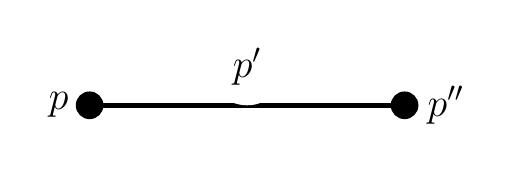
\begin{tikzpicture}[shorten >=1pt, auto, node distance=3cm, ultra thick]
   \begin{scope}[every node/.style={circle,draw=white,fill=white!20!,font=\sffamily\Large\bfseries}]
\coordinate(a) at (0,0);
\coordinate(b) at (4,0);
\draw (a)--(b);
\node [left]  at (a) {$p$};
\node [right]  at (b) {$p^{\prime \prime}$};
\draw  (a) edge node{$p^{\prime}$} (b);
\foreach \p in {a,b}
       \fill [black] (\p) circle (5pt);
  \end{scope}
\end{tikzpicture}
}
\caption{Single link with simultaneous node/link failures. \label{rvrI}}
\end{center}
\end{figure}

\begin{table}[H]
\caption{RVR Validation Test: single link} % title of Table
\centering  % used for centering table
\begin{tabular}{|c|c|c|c|c|} % centered columns 
\hline	$Instance$   &	$R_{s,t}$ & $\hat{R}$&  $\hat{V}$ \\
\hline	$p=p^{\prime}=p^{\prime \prime}=0.9$	& $0.729$ &	$0.729$ 	&	$3.13631E-17$	\\
\hline
\end{tabular}
\label{rvrTable1} % is used to refer this table in the text
\end{table}


\subsubsection*{Case II: Two-Path}
The second test consists of an elementary path composed by two links, with elementary reliability $p^{\prime}$. 
The end-points have reliability $p$, while the central point has reliability $p^{\prime \prime}$ 
(see Figure~\ref{rvrII}). The source-terminal reliability between the end-points is 
$R_{s,t}=p^2(p^{\prime})^2 p^{\prime \prime}$. Table~\ref{rvrTable2} shows a small gap between 
the correct value $R_{s,t}$ and its estimation $\hat{R}$. The estimated variance is reduced as well.

\begin{figure}[H]
\begin{center}
\scalebox{1}{
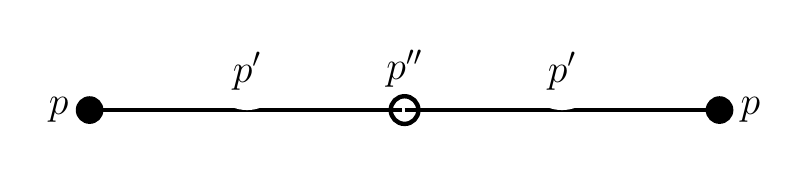
\begin{tikzpicture}[shorten >=1pt, auto, node distance=3cm, ultra thick]
   \begin{scope}[every node/.style={circle,draw=white,fill=white!20!,font=\sffamily\Large\bfseries}]
\coordinate(a) at (0,0);
\coordinate(b) at (4,0);
\coordinate(c) at (8,0);

\draw (a)--(b);
\draw (b)--(c);

\node [left]  at (a) {$p$};
\node [above]  at (b) {$p^{\prime \prime}$};
\node [right]  at (c) {$p$};

\draw  (a) edge node{$p^{\prime}$} (b);
\draw  (b) edge node{$p^{\prime}$} (c);

\foreach \p in {a,c}
       \fill [black] (\p) circle (5pt);
\foreach \p in {b}
       \draw (\p) circle (5pt);
  \end{scope}
\end{tikzpicture}
}      
\caption{Elementary path with simultaneous node/link failures. \label{rvrII}}
\end{center}
\end{figure}

\begin{table}[H]
\caption{RVR Validation Test: elementary path} % title of Table
\centering  % used for centering table
\begin{tabular}{|c|c|c|c|c|} % centered columns 
\hline	$Instance$   &	$R_{s,t}$ & $\hat{R}$&  $\hat{V}$ \\
\hline	$p=p^{\prime}=p^{\prime \prime}=0.9$	& $0.59049$ &	$0.593354$ 	&	$3.3341E-06$	\\
\hline
\end{tabular}
\label{rvrTable2} % is used to refer this table in the text
\end{table}

In the following cases we consider perfect terminals only, with possible failures of Steiner nodes. 
\subsubsection*{Case III: Triangle}
Consider the complete graph composed by three terminal-nodes, or the triangle $K_3$, 
with identical elementary link-reliabilities $p$ (see Figure~\ref{rvrIII}). 
A complete graph with high elementary reliabilities for both links and nodes is therefore highly-reliable. Observe that if two or more links fail, the system is down. 
Otherwise, the system works. By elementary combinatorics, the all-terminal reliability 
is in this case $R_V = \binom{3}{0}p^3+ \binom{3}{1}p^2(1-p) = p^3+3p^2(1-p)$, where the first term means that 
\emph{no link fails}, and the second means that \emph{precisely one link fails}. From Table~\ref{rvrTable3} 
we can observe that the gap between $R_{V}$ and $\hat{R}$ is smaller than $10^{-3}$, and the 
variance is extremely small, showing a good performance of RVR, as expected for small-sized networks. 

\begin{figure}[H]
\begin{center}
\scalebox{1}{
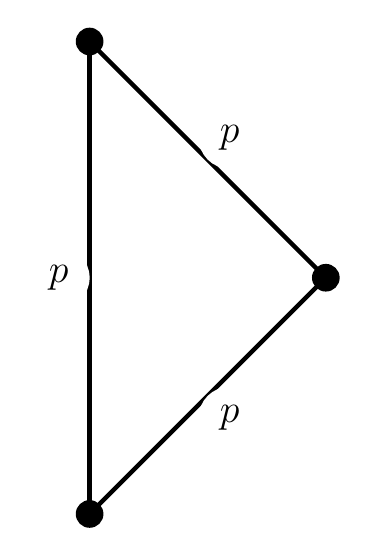
\begin{tikzpicture}[shorten >=1pt, auto, node distance=3cm, ultra thick]
   \begin{scope}[every node/.style={circle,draw=white,fill=white!20!,font=\sffamily\Large\bfseries}]
\coordinate(a) at (0,0);
\coordinate(b) at (0,6);
\coordinate(c) at (3,3);
\draw  (a) edge node{$p$} (b);
\draw  (b) edge node{$p$} (c);
\draw  (c) edge node{$p$} (a);
\foreach \p in {a,b,c}
       \fill [black] (\p) circle (5pt);
  \end{scope}
\end{tikzpicture}
}
\caption{Triangle with link failures. \label{rvrIII}}
\end{center}
\end{figure}

\begin{table}[H]
\caption{RVR Validation Test: Triangle} % title of Table
\centering  % used for centering table
\begin{tabular}{|c|c|c|c|c|} % centered columns 
\hline	$Instance$   &	$R_{V}$ & $\hat{R}$&  $\hat{V}$ \\
\hline	$p=0.9$	& $0.972$ &	$0.972473$ 	&	$6.21454E-08$	\\
\hline
\end{tabular}
\label{rvrTable3} % is used to refer this table in the text
\end{table}

\subsubsection*{Case IV: Triangle with a pending link}
Consider a triangle with a pending link presented in Figure~\ref{rvrIV}, where the central node is a Steiner node (and a cut-point, since it disconnect the network if fails). The $K$-terminal reliability depends strongly on the operational reliabilities of the central node and the bridge. A straight calculation leads to see that 
$R_K = p^{\prime}p^{\prime \prime} [p^3+3p^{2}(1-p)]$. From Table~\ref{rvrTable4}, we can appreciate 
that the gaps in the reliability is again smaller than $10^{-3}$, and the variance of the estimator is really small. 

\begin{figure}[H]
\begin{center}
\scalebox{1}{
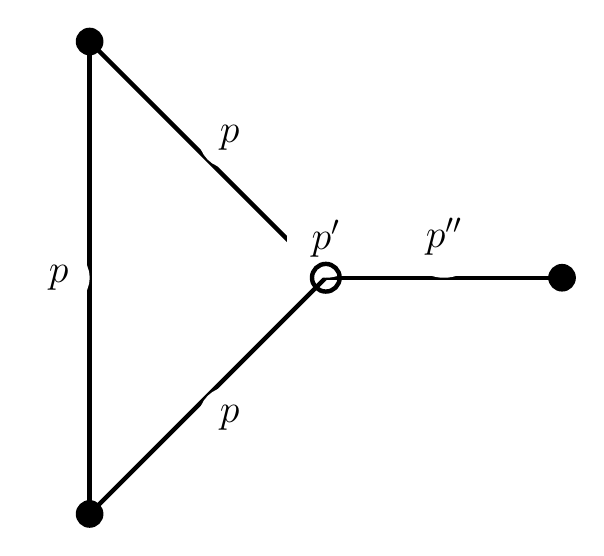
\begin{tikzpicture}[shorten >=1pt, auto, node distance=3cm, ultra thick]
   \begin{scope}[every node/.style={circle,draw=white,fill=white!20!,font=\sffamily\Large\bfseries}]
\coordinate(a) at (0,0);
\coordinate(b) at (0,6);
\coordinate(c) at (3,3);
\coordinate(d) at (6,3);

\draw  (a) edge node{$p$} (b);
\draw  (b) edge node{$p$} (c);
\draw  (c) edge node{$p$} (a);
\draw  (c) edge node{$p^{\prime \prime}$} (d);
\node [above]  at (c) {$p^{\prime}$};

\foreach \p in {a,b,d}
       \fill [black] (\p) circle (5pt);
\foreach \p in {c}
       \draw (\p) circle (5pt);
  \end{scope}
\end{tikzpicture}
}
\caption{Triangle with pending link. Potential failure in central node. \label{rvrIV}}
\end{center}
\end{figure}

\begin{table}[H]
\caption{RVR Validation Test: Triangle with a pending link} % title of Table
\centering  % used for centering table
\begin{tabular}{|c|c|c|c|c|} % centered columns 
\hline	$Instance$   &	$R_{K}$ & $\hat{R}$&  $\hat{V}$ \\
\hline	$p=0.9$, $p^{\prime}=0.5$, $p^{\prime \prime}=0.9$	& $0.4374$ &	$0.438066$ 	&	$3.18052E-07$	\\
\hline	$p=0.9$, $p^{\prime}=0.9$, $p^{\prime \prime}=0.5$		& $0.4374$ &	$0.437479$ 	&	$4.32176E-07$	\\
\hline
\end{tabular}
\label{rvrTable4} % is used to refer this table in the text
\end{table}

\subsubsection*{Case V: Tree}
Consider the tree from Figure~\ref{rvrV}, where the terminals are the leaf-nodes, and all the links and 
Steiner nodes operate independently, with identical reliability. 
In a tree, the failure of only component disconnects some pair of leaf-nodes. Consequently, the reliability 
of trees with several components is reduced, and it is the product of all the elementary reliabilities of its components: $R_K = p^9$. From Table~\ref{rvrTable5}, we can appreciate that both the reliability gap and the variance are greater than in the previous cases. 

\begin{figure}[H]
\begin{center}
\scalebox{1}{
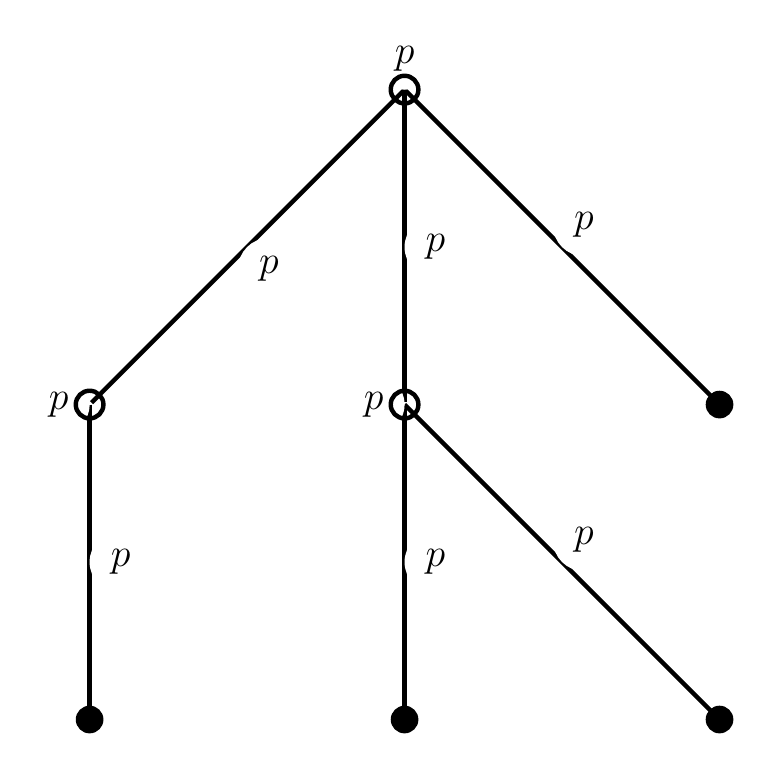
\begin{tikzpicture}[shorten >=1pt, auto, node distance=3cm, ultra thick]
   \begin{scope}[every node/.style={circle,draw=white,fill=white!20!,font=\sffamily\Large\bfseries}]
\coordinate(a) at (0,8);
\coordinate(b) at (4,4);
\coordinate(c) at (0,4);
\coordinate(d) at (-4,4);
\coordinate(e) at (4,0);
\coordinate(f) at (0,0);
\coordinate(g) at (-4,0);

\draw  (a) edge node{$p$} (b);
\draw  (a) edge node{$p$} (c);
\draw  (a) edge node{$p$} (d);
\draw  (c) edge node{$p$} (f);
\draw  (c) edge node{$p$} (e);
\draw  (d) edge node{$p$} (g);

\node [above]  at (a) {$p$};
\node [left]  at (c) {$p$};
\node [left]  at (d) {$p$};

\foreach \p in {b,e,f,g}
       \fill [black] (\p) circle (5pt);
\foreach \p in {a,c,d}
       \draw (\p) circle (5pt);
  \end{scope}
\end{tikzpicture}
}
\caption{Tree with failures in links and non-leaf nodes. \label{rvrV}}
\end{center}
\end{figure}

\begin{table}[H]
\caption{RVR Validation Test: Tree-graph} % title of Table
\centering  % used for centering table
\begin{tabular}{|c|c|c|c|c|} % centered columns 
\hline	$Instance$   &	$R_{K}$ & $\hat{R}$&  $\hat{V}$ \\
\hline	$p=0.9$	& $0.387420489$ &	$0.391676$ 	&	$1.53487e-05$	\\
\hline
\end{tabular}
\label{rvrTable5} % is used to refer this table in the text
\end{table}


\subsubsection*{Case VI: Wheatstone Bridge}
In the Wheatstone Bridge from Figure~\ref{rvrVI}, our measure of interest is the source-terminal reliability 
$R_{s,t}$. It strongly depends on the elementary node-reliability $p^{\prime}$ of Steiner nodes, since these 
represent intermediate nodes. By an exhaustive enumeration of pathsets, a closed-form for the reliability can be obtained:
\begin{equation*}
R_{s,t}= p^2p^{\prime} + p^2(1-p)p^{\prime} + p^3p^{\prime}(1-p^{\prime}) + (1-p)p^3(p^{\prime})^2 + 
p^3(1-p)^2(p^{\prime})^2+ p^3(1-p)^2(p^{\prime})^2.
\end{equation*}

From Table~\ref{rvrTable6}, we conclude that the reliability gaps and variance are acceptable. 
\begin{figure}[H]
\begin{center}
\scalebox{1}{
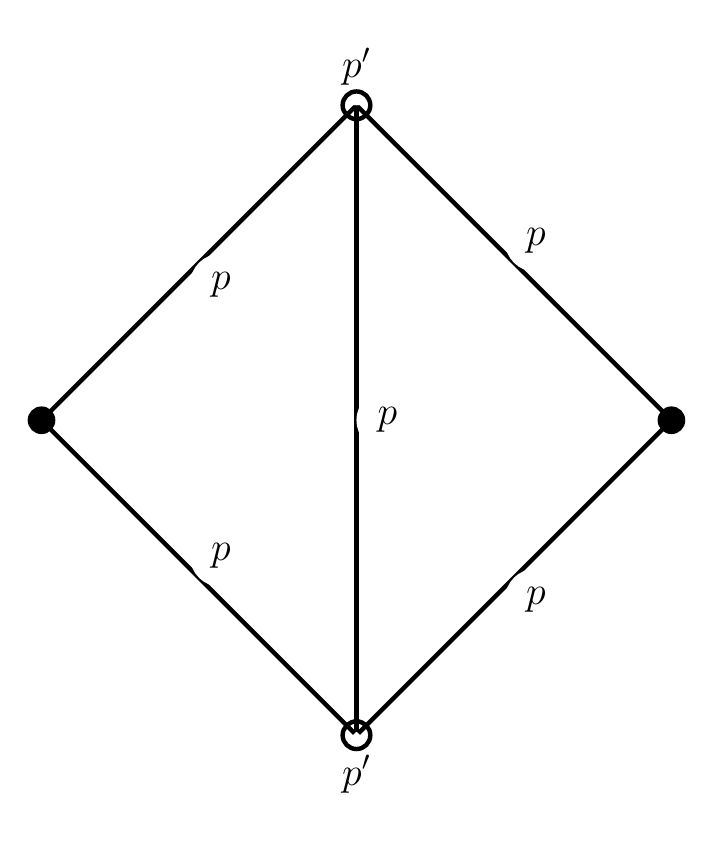
\begin{tikzpicture}[shorten >=1pt, auto, node distance=3cm, ultra thick]
   \begin{scope}[every node/.style={circle,draw=white,fill=white!20!,font=\sffamily\Large\bfseries}]
\coordinate(a) at (0,8);
\coordinate(b) at (4,4);
\coordinate(c) at (-4,4);
\coordinate(d) at (0,0);

\draw  (a) edge node{$p$} (b);
\draw  (a) edge node{$p$} (c);
\draw  (a) edge node{$p$} (d);
\draw  (c) edge node{$p$} (d);
\draw  (b) edge node{$p$} (d);

\node [above]  at (a) {$p^{\prime}$};
\node [below]  at (d) {$p^{\prime}$};


\foreach \p in {b,c}
       \fill [black] (\p) circle (5pt);
\foreach \p in {a,d}
       \draw (\p) circle (5pt);
  \end{scope}
\end{tikzpicture}
}
\caption{Wheatstone Bridge with failures in links and a couple of nodes. \label{rvrVI}}
\end{center}
\end{figure}

\begin{table}[H]
\caption{RVR Validation Test: Wheatstone Bridge} % title of Table
\centering  % used for centering table
\begin{tabular}{|c|c|c|c|c|} % centered columns 
\hline	$Instance$   &	$R_{K}$ & $\hat{R}$&  $\hat{V}$ \\
\hline	$p=0.9$, $p^{\prime}=0.5$	& $0.64962$ &	$0.654653$ 	&	$6.7791E-06$	\\
\hline	$p=0.9$, $p^{\prime}=0.9$	& $0.9383688$ &	$0.937484$ 	&	$1.89235E-06$	\\
\hline
\end{tabular}
\label{rvrTable6} % is used to refer this table in the text
\end{table}

\subsubsection*{Comments on the Results}
Several validation tests were carried out using different elementary reliabilities for nodes and links. 
Some errors were detected during the validation tests, which served to correct the implementation of RVR with 
the corresponding logical modifications. Double-precision arithmetic was used for the operations, with up to 15 digits.
%  \input{apendice/apendice_B}
%  \input{apendice/apendice_C}
  
%  \anexarabicnumbering
%  \anexmatter
%  \input{anexo/anexo_A}
\listoffigures	         % Lista de figuras
  
\end{document}

% ===== FIN DEL DOCUMENTO =====